% Lump tex of Xiaojun's defense slides

\documentclass[xcolor=dvipsnames]{beamer}
%%\usetheme{default}
\usecolortheme[named=Maroon]{structure}
%\usetheme{Boadilla}
\usetheme{Madrid}
\useoutertheme{default}%[footline=empty]{infolines}

% \usepackage{helvet}
% \usepackage{enumerate}
% \usepackage{amsmath}
% \usepackage{amsfonts}
% \usepackage{graphicx}
% \usepackage{ulem}
\usepackage{multirow}
\usepackage{comment}
\usepackage{xspace}
\usepackage{polynom}
%\usepackage{columns}

\usepackage[absolute,overlay]{textpos}
\usepackage[ruled,linesnumbered]{../algorithm2e}
%%for algorithm2e package, label has to be following caption in the same line!!!
\renewcommand{\algorithmcfname}{ALGORITHM}
\renewcommand{\thealgocf}{}
\SetAlFnt{\small}
\SetAlCapFnt{\small}
\SetAlCapNameFnt{\small}
\SetAlCapHSkip{0pt}
\IncMargin{-\parindent}

%\RequirePackage{algorithmic}
%\RequirePackage{algorithm}
% \renewcommand{\algorithmicrequire}{\textbf{Inputs:}}
% \renewcommand{\algorithmicensure}{\textbf{Outputs:}}


%\newtheorem{theorem}{Theorem}
%\newtheorem{lemma}{lemma}
%\newtheorem{corollary}{Corollary}
%\newtheorem{proposition}{Proposition}
%\newtheorem{Q}{Question}
%\newtheorem{Exa}{Example}
%\newtheorem{Definition}{Definition}


\newcommand{\Fq}{{\mathbb{F}}_{q}}
\newcommand{\Fp}{{\mathbb{F}}_{p}}
\newcommand{\Fpk}{{\mathbb{F}}_{p^k}}
\newcommand{\Fkk}{{\mathbb{F}}_{2^k}}
\newcommand{\Z}{{\mathbb{Z}}}
\newcommand{\Zkk}{{\mathbb{Z}}_{2^k}}
\newcommand{\Fkkx}[1][x]{\ensuremath{\mathbb{F}}_{2^k}[#1]\xspace}
\newcommand{\Grobner}{Gr\"{o}bner\xspace}
%\newcommand{\Grobner}{Gr\"{o}bner}
\newcommand{\bi}{\begin{itemize}}
\newcommand{\ei}{\end{itemize}}
\newcommand{\Func}{{\mathcal{F}}}
\newcommand{\N}{{\mathcal{N}}}
\newcommand{\G}{{\mathcal{G}}}
\newcommand{\F}{{\mathbb{F}}}
\newcommand{\B}{{\mathbb{B}}}
\newcommand{\C}{{\mathbb{C}}}
\newcommand{\R}{{\mathbb{R}}}

\title[PhD Dissertation Defense]{Word-Level Abstractions for Sequential Design Verification using Algebraic Geometry}

\author[Xiaojun Sun]{{\bf Xiaojun Sun}, PhD Candidate}

%\email{rostamian@umbc.edu}
\institute[Univ. of Utah]{

\includegraphics[height=22mm]{./Ulogo_1200px.png}\\
\    \\
\    \\
\    \\
Electrical and Computer Engineering, University of Utah\\
\    \\
Advisor: {\it Priyank Kalla}
}

\date{Dec 16, 2016}

%%%%%%%%%%%%%%%%%%%%%%%%%%%%%%%%%%%%%%%%%%%%%%%%%%
%%%%%%%%%%%%%%%%%%%%%%%%%%%%%%%%%%%%%%%%%%%%%%%%%%
%%%%%%%%%%%%%%%%%%%%%%%%%%%%%%%%%%%%%%%%%%%%%%%%%%
\begin{document}
%----------- titlepage ----------------------------------------------%
\begin{frame}[plain]
  \titlepage

\end{frame}

%\maketitle
%%%%%%%%%%%%%%%%%%%%%%%%%%%%%%%%%%%%%%%%%%%%%%%%%%
\begin{frame}{\large{Outline}}
\bi
\item Contributions
\item Motivations
\item Previous Work
\item Preliminaries
	\bi
	\item Finite fields
	\item Polynomial algebra \& Algebraic geometry
	\item Projection of varieties
	\ei
\item Projection based abstraction 
	\bi 
	\item Application: \alert{Reachability analysis}
	\item Application: \alert{Sequential arithmetic ckt verification}
	\ei
\item UNSAT core based abstraction
	\bi
	\item \alert{UNSAT core extraction using Gr\"obner basis refutation}
	\item Application: Bounded model checking (BMC) with abstraction refinement
	\ei
\item Conclusion \& Future work
\ei
\end{frame}
%%%%%%%%%%%%%%%%%%%%%%%%%%%%%%%%%%%%%%%%%%%%%%%%%%
\begin{frame}{\large{Contributions}}
\bi
\item Word-level reachability analysis -- analog of implicit state enumeration
	\bi 
	\item {\bf Q:} Why word-level? 
	\pause
	\item {\bf A:} Data $\gets$ word-level info 
	\pause
	\item {\bf A:} Simplify representation (abstraction) of state-space $\to$ Efficiency!
	\ei
\pause
\item Apply word-level reachability algorithm to sequential arithmetic circuit verification
	\bi
	\item Abstraction $\to$ word-level signature each time-frame
	\bi
            \item Word-level abstraction from bit-level ckts [Pruss, 2015]
        \ei
	\item Word-level unrolling
	\ei
\pause
\item UNSAT cores in Algebraic geometry
	\bi
	\item Analyze Buchberger's algorithm $\to$ extract refutation proof $\to$ UNSAT core
	\item Structure of refutation proof $\to$ refine UNSAT core
	\ei
\pause
\item Implement above algos: C++ \& \textsc{Singular}
	\bi
	\item For sequential GF multipliers: overwhelmingly better than contemporary tools
	\ei
\ei
\end{frame}
%%%%%%%%%%%%%%%%%%%%%%%%%%%%%%%%%%%%%%%%%%%%%%%%%%%%
\begin{frame}[label = linkSTG]{\large{Motivation I: BFS state space traversal}}
\begin{columns}[onlytextwidth]
\begin{column}{0.5\textwidth}
\begin{figure}
\centering
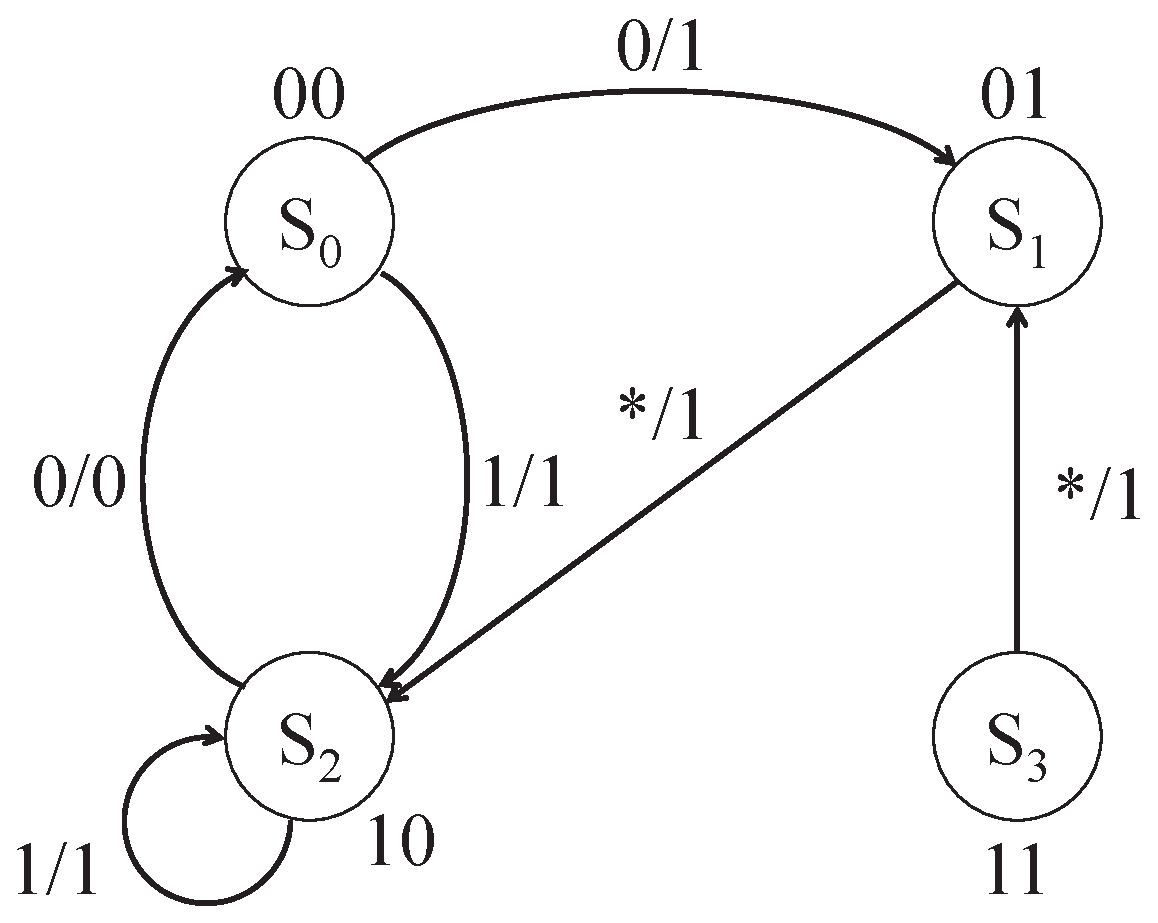
\includegraphics[scale=0.25]{./stg_fig.eps}
\caption{State Transition Graph}
\end{figure}
\hyperlink{pptpage2}{\beamergotobutton{Go back to example}}
\end{column}
\begin{column}{0.5\textwidth}
\bi
\item Initial state: $\{00\}$
\item Iteration 1: 
	\bi
	\item Start from $\{00\}$
	\item One-step transition: $\{01,10\}$
	\item Newly reached: $\{01,10\}$
	\ei
\item Iteration 2: 
	\bi
	\item Start from $\{01,10\}$
	\item One-step transition: $\{00,10\}$
	\item Newly reached: $\emptyset$
	\ei
\item All reachable states detected. Final reached states: $\{00,01,10\}$
\pause
\item Still need bit-level Boolean variables to represent states
\ei
\end{column}
\end{columns}

\end{frame}
%%%%%%%%%%%%%%%%%%%%%%%%%%%%%%%%%%%%%%%%%%%%%%%%%%%%%
\begin{frame}[label = motiv2]{\large{Motivation II: Sequential arithmetic circuits verification}}
\vspace{-0.1in}
\begin{figure}[H]
\centering{
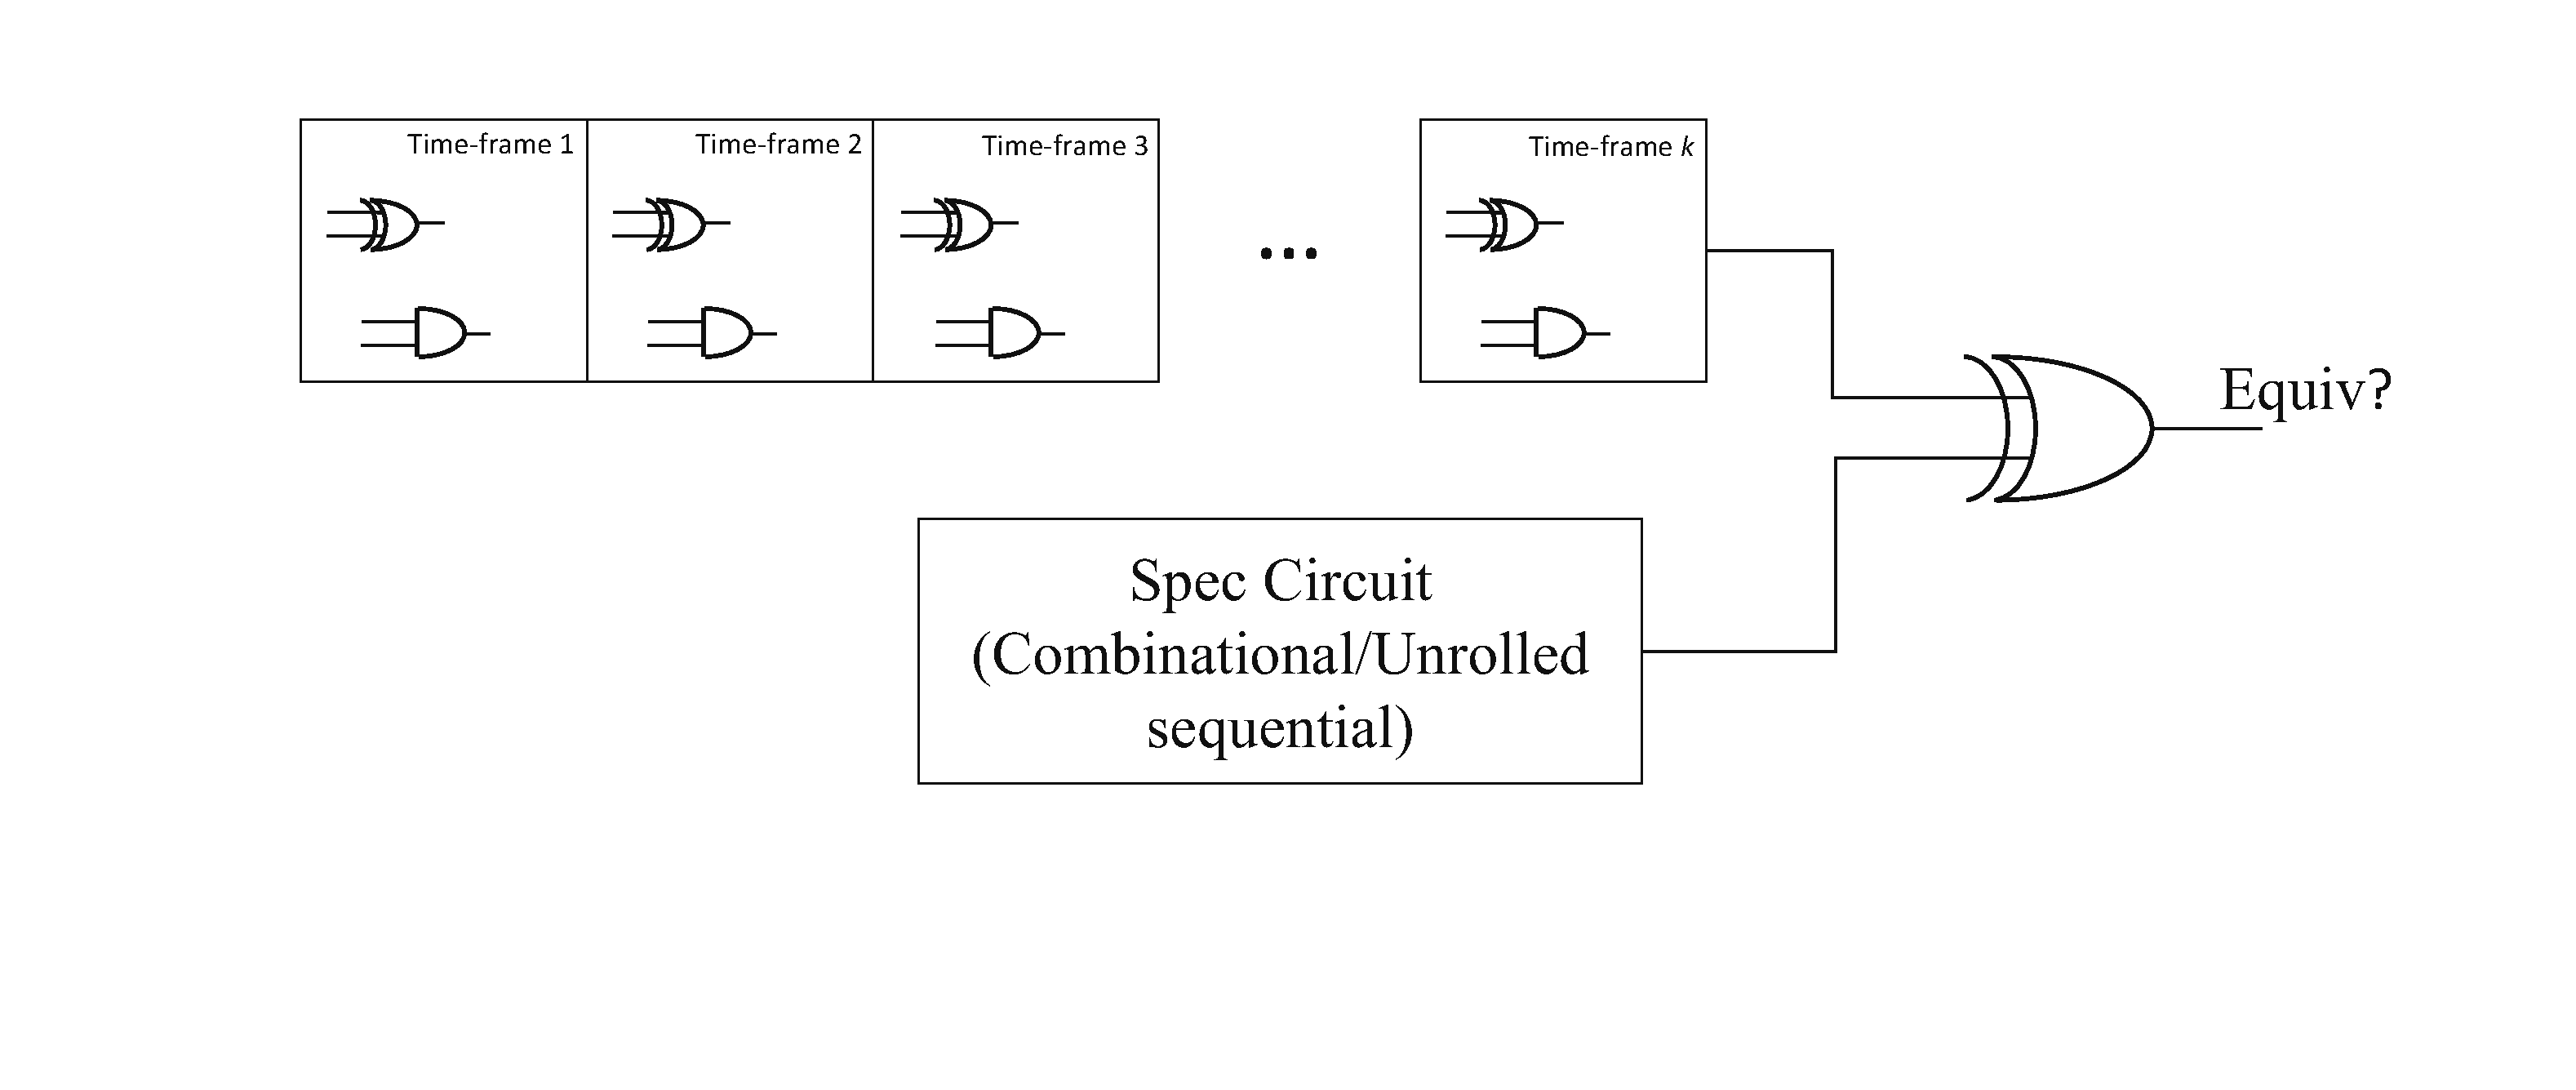
\includegraphics[width=4.5in]{../newfig/convention.eps}
}
\end{figure}
\vspace{-0.2in}
\bi
\item Problem: Verify the function of sequential arithmetic circuit
	\bi
	\item Operands preloaded into registers
	\item After $k$ clock cycles, give desired output
	\ei
\item Conventional: explicitly unroll $k$ time-frames (bit-level) and setup miter
	\bi
	\item Check miter output: SAT, BDDs, AIGs
	\item Bit-blasting!
	\ei
\ei
\hyperlink{Moore}{\beamergotobutton{Go back to Moore machine}}
\hyperlink{expSMPO}{\beamergotobutton{Go back to Exp result}}
\end{frame}
%%%%%%%%%%%%%%%%%%%%%%%%%%%%%%%%%%%%%%%%%%%%%%%%%%%%%%%
\begin{frame}[label = motiv3]{\large{Motivation III: $k$-BMC with abstraction refinement}}
\IncMargin{1em}
\begin{algorithm}[H]
\SetAlgoNoLine
	\KwIn{$M$ is the original machine, $p$ is the property to check, $k$ is the number of steps unrolling $M$}
  $k = $ InitValue\;
  \eIf{$k$-BMC$(M,p,k)$ is \textbf{SAT} (reachable states after $k$ steps violates $p$)}
  {
	\Return{``Found error trace"}
  }
  {
	\alert{Extract UNSAT core $\mathcal P$ of $k$-BMC} \;
	$M' = $ \textit{ABSTRACT}$(M,\mathcal P)$\;
  }
  \eIf{MODEL-CHECK$(M',p)$ returns \textbf{PASS}}
  {
	\Return{``Passing property"}
  }
  {
	Increase bound $k$\;
	goto Line 2\;
  }
\caption{$k$-BMC with Abstraction Refinement (L. Zhang'05)}
\end{algorithm}
\DecMargin{1em}
\hyperlink{refine}{\beamergotobutton{Go back to Abs refine}}
\end{frame}
%%%%%%%%%%%%%%%%%%%%%%%%%%%%%%%%%%%%%%%%%%%%%%%%%%%%%%%%
\begin{frame}{\large{Previous work}}
\bi
\item Sequential Equivalence Checking (SEC): bit-blasting, or structural info dependency
	\bi
	\item Usually based on reachability analysis
	\item Sequential miter
	\item Unroll, then use DDs, SAT or AIGs (Combinational)
	\item Induction-based
	\ei
\item Symbolic model checking (counterexample, IC3): SAT/BDDs in nature
\item Word-level techniques (term rewriting, uninterpreted function): no universal representation/no encoding
\item Algebraic geometry methods
	\bi
	\item Gr\"ober basis in model checking [Avrunin,CAV'96;Vardi,IASTED'07]: Analog of bit-level Boolean functions
	\item Abstract word-level polynomial representation for arbitrary combinational ckt [Pruss,TCAD'16]
	\ei
\pause
\item No purely word-level sequential verification: data/abstraction/algorithm
\ei
\end{frame}
%%%%%%%%%%%%%%%%%%%%%%%%%%%%%%%%%%%%%%%%%%%%%%%%%%%%%%%
\begin{frame}{\large{Working field: $\Fkk$}}
\bi
\item Our proposed state-space model is based on finite field $\Fkk$
	\bi
	\item $\B^k$: bit-vector
	\item $\Z_{2^k}$, $\R$: approaches not compatible
	\ei
\item Evaluations in $\B^k \Leftrightarrow$ Elements in $\Fkk$
\item Functions $\B^k\to\B^k \Leftrightarrow \Func:\Fkk\to\Fkk$
\pause
\item State-space: finite set of $2^k$ points
\item Treat them as solutions to polys in $\Fkk$
\ei
\end{frame}
%%%%%%%%%%%%%%%%%%%%%%%%%%%%%%%%%%%%%%%%%%%%%%%%%%%%%%%%
\begin{frame}{\large{Preliminaries: Finite/Galois Fields}}
\textbf {Galois field} $\mathbb{F}_q$ is a finite field with $q$
elements, $q = p^k$, $p = $prime
\begin{itemize}
\item 0,1 elements, commutative, associate, distributive laws
\item Closure property: $+,-,\times$, inverse ($\div$)
\end{itemize}


Our interest: $\mathbb{F}_{q} = \Fkk$ ($q = 2^k$)
\begin{itemize}
\item  $\mathbb{F}_{2^k}$: $k$-dimensional extension of  $\mathbb{F}_{2}=\{0,1\}$
	\begin{itemize}
	\item $k$-bit bit-vector, AND/XOR arithmetic
	\end{itemize}
\end{itemize}

To construct $\mathbb{F}_{2^k}$
\begin{itemize}
\item $\mathbb{F}_{2^k} \equiv \mathbb{F}_{2}[x] \pmod {P(x)}$
\item $P(x) \in \mathbb{F}_{2}[x]$, irreducible polynomial of degree $k$
\item Root $P(x)=0$: primitive element
\bi
\item E.g. $\C   = \R[x] \pmod{ x^2+1}$
\ei
\item Operations performed (mod $P(x)$) and coefficient reduced (mod 2)

\end{itemize}
\end{frame}
%%%%%%%%%%%%%%%%%%%%%%%%%%%%%%%%%%%%%%%%%%%%%%%%%%%%%%%%%
\begin{frame}{Preliminaries: Field construction of $\mathbb{F}_8$}
%\ptsize{10}

Consider: $\mathbb{F}_{2^3}= \mathbb{F}_{2}[x] \pmod {x^3 + x +
  1}$\\ $A \in \mathbb{F}_{2}[x]$ \\ 
$A \pmod {x^3 + x + 1} = a_2 x^2 + a_1 x + a_0$. Let $P(\alpha) = 0$:

\begin{itemize}
\item $\langle a_2, a_1, a_0 \rangle = \langle 0, 0, 0\rangle = 0$
\item $\langle a_2, a_1, a_0 \rangle = \langle 0, 0, 1\rangle = 1$
\item $\langle a_2, a_1, a_0 \rangle = \langle 0, 1, 0\rangle = \alpha$
\item $\langle a_2, a_1, a_0 \rangle = \langle 0, 1, 1\rangle = \alpha
  + 1$
\item $\langle a_2, a_1, a_0 \rangle = \langle 1, 0, 0\rangle = \alpha^2$
\item $\langle a_2, a_1, a_0 \rangle = \langle 1, 0, 1\rangle =
  \alpha^2 + 1$
\item $\langle a_2, a_1, a_0 \rangle = \langle 1, 1, 0\rangle =
  \alpha^2 + \alpha$
\item $\langle a_2, a_1, a_0 \rangle = \langle 1, 1, 1\rangle =
  \alpha^2 + \alpha + 1$
\end{itemize}
\end{frame}
%%%%%%%%%%%%%%%%%%%%%%%%%%%%%%%%%%%%%%%%%%%%%%%%%%%%%%%%%
\begin{frame}{\large{Preliminaries: Polynomial function $f:\Fq\to\Fq$}}

\begin{Theorem}[Fermat's Little Theorem over $\Fq$]
Let $\alpha \in \Fq$, then $\alpha^q = \alpha$. Therefore, $x^q -x$
vanishes on all points in $\Fq$. 
\end{Theorem}
\begin{table}[H]
\label{tab:truthtable}
\centering{\small
\begin{tabular}{|c|ccc|c|}
\hline
$\{a_2a_1a_0\}\in\mathbb{B}^3$   & $A\in \F_{2^3}$ &$\rightarrow$& $\{z_2z_1z_0\}\in\mathbb{B}^3$  & $Z\in \F_{2^3}$ \\
\hline
000  &0 &$\rightarrow$&000 & 0 \\
001  &1 &$\rightarrow$&001 & 1 \\
010  &$\alpha$ & $\rightarrow$ & 111& $\alpha^2 + \alpha + 1$ \\
011  &$\alpha + 1$ &$\rightarrow$& 111 & $\alpha^2 + \alpha + 1$ \\
100  &$\alpha^2$ &$\rightarrow$& 101 &  $\alpha^2+1$ \\
101  &$\alpha^2 + 1$ &$\rightarrow$&011 & $\alpha+1$ \\
110  &$\alpha^2 + \alpha$&$\rightarrow$& 101 &$\alpha^2 + 1$ \\
111  &$\alpha^2 + \alpha + 1$ &$\rightarrow$& 101 &$\alpha^2 + 1$\\
\hline
\end {tabular}
}
\caption{Truth table for mappings in $\mathbb{B}^3$ and $\F_{2^3}$}
\end{table}
\pause
\vspace{-0.2in}
% \bi
% \item Always possible to generate word-level poly function using Lagrange's interpolation
% \ei
\begin{align*}
Z =& \Func(A) \\
=& (\alpha^2+\alpha+1) A^7 + (\alpha^2+1) A^6 + \alpha A^5 + (\alpha+1) A^4 \\
&+ (\alpha^2+\alpha+1)A^3+ (\alpha^2+1)A
\end{align*}
\end{frame}
%%%%%%%%%%%%%%%%%%%%%%%%%%%%%%%%%%%%%%%%%%%%%%%%%%%%%%%%%%%%%
\begin{frame}{\large{Preliminaries: Computer algebra terminology}}
\vspace{-0.2in}
%\ptsize{10}
Let $\mathbb{F}_q = GF(2^k)$, and $\overline{\Fq}$ be its closure
\begin{itemize}
\item $\mathbb{F}_q[x_1, \ldots, x_n]$: ring of all polynomials with
  coefficients in $\mathbb{F}_q$ 

\item Polynomial $f = c_1X_1 + c_2 X_2 + \dots + c_t X_t$
\bi
\item A monomial ordering is imposed on $f: X_1 > X_2 > \dots > X_t$
\item \alert{Leading term} $lt(f) = c_1 X_1, ~~tail(f) = c_2 X_2 + \dots + c_t X_t$
\item Leading coefficient $lt(f) = c_1$ and leading monomial $lm(f) = X_1$
\ei
\begin{itemize}
\item LEX $x> y> z$: ~~$f = \alert{ -2x^3} + 2x^2yz + 3xy^3$
\item  DEGLEX $x>y>z$:  ~~$f = \alert{ 2x^2yz} + 3xy^3 -2x^3$
\item DEGREVLEX $x>y>z$: ~~$f = \alert{3xy^3} + 2x^2yz - 2x^3$
\end{itemize}
\end{itemize}
\bi
\item Leading terms $lt(f)$ play an important role
\bi
\item Affect division results!
\ei
\ei

\end{frame}
%%%%%%%%%%%%%%%%%%%%%%%%%%%%%%%%%%%%%%%%%%%%%%%%%%%%%%%%%%%%%%
\begin{frame}{\large{Preliminaries: Polynomial division}}
Divide $f = x^3-2x^2+2x+8$ ~~by ~~$g =2x^2+3x + 1$\\

\pause

\polylongdiv{x^3-2x^2+2x+8}{2x^2+3x + 1}

\pause

\bi
\item The key step in division: \alert{$r = f - \frac{lt(f)}{lt(g)}\cdot  g$}, denoted $f\xrightarrow{g} r$
\item Similarly divide $f$ by a set of polynomials $F = \{f_1,\dots, f_s\}$
\item Denoted: $f \xrightarrow{f_1, \dots, f_s}_+ r$
\bi
\item Remainder $r$ is reduced: no term in $r$ is divisible by $lt(f_i)$
\ei
\ei
\end{frame}
%%%%%%%%%%%%%%%%%%%%%%%%%%%%%%%%%%%%%%%%%%%%%%%%%%%%%%%%%%%%%%
\begin{frame}{\large{Preliminaries: Algebraic geometry terminology (cont.)}}
Let $\mathbb{F}_q = GF(2^k)$:
\begin{itemize}
% \item $\mathbb{F}_q[x_1, \ldots, x_n]$: ring of all polynomials with
%   coefficients in $\mathbb{F}_q$ 
\item Given a set of polynomials:
\begin{itemize}
\item $f_1, f_2, \dots , f_s \in \mathbb{F}_q[x_1, \dots, x_n]$
\item Find solutions to $f_1 = f_2 = \dots = f_s = 0$
\end{itemize}
\item \alert{Variety:} Set of ALL solutions to a given system of polynomial equations: $V(f_1, \dots, f_s)$
	\begin{itemize}
	\item In $\mathbb{R}\left[x,y\right]$, $V(x^2+y^2-1)=\{all\  points\  on\ circle: x^2+y^2-1=0\}$
	\item In $\mathbb{R}[x]$, $V(x^2+1)=\emptyset$
	\item In $\mathbb{C}[x]$, $V(x^2+1)=\{(\pm i)\}$
	\end{itemize}
\item Variety depends on the \alert{ideal} generated by the polynomials.
\item Reason about the Variety by analyzing the Ideals
\end{itemize}
\end{frame}

%%%%%%%%%%%%%%%%%%%%%%%%%%%%%%%%%%%%%%%%%%%%%%%%%%%%%%%%%%%%%%%%
\begin{frame}{\large{Preliminaries: Ideals \& Gr\"obner bases}}
\vspace{-0.1in}


\begin{Definition}
{\bf Ideals of Polynomials:} Let $f_1, f_2, \ldots, f_s \in
\mathbb{F}_q[x_1, \dots, x_n]$. Let 
\begin{eqnarray}
J = \langle f_1, f_2 \ldots, f_s\rangle = \{f_1 h_1 + f_2 h_2 + \dots + f_s h_s\},~~h_i\in\Fq[x_1,\dots,x_n] \nonumber 
\end{eqnarray}

$J = \langle f_1, f_2 \ldots, f_s\rangle$ is an ideal generated by
$f_1, \ldots, f_s$ and the polynomials are called the generators. 
\end{Definition}

\vspace{-0.1in}
%\ptsize{10}

\begin{itemize}
\item Different generators can generate the same ideal
\item $\langle f_1,\cdots,f_s \rangle=\cdots=\langle g_1,\cdots,g_t
  \rangle$
\item Some generators are a ``better'' representation of the ideal
\item A {\bf Gr\"obner basis} $G$ is a ``canonical'' representation of an ideal
	\bi
	\item $I = \langle F \rangle = \langle G \rangle$, and $V(F)=V(G)$
	\ei
\item Map: set of states $\to$ \alert{variety} of polynomial ideal
\end{itemize}
\end{frame}
%%%%%%%%%%%%%%%%%%%%%%%%%%%%%%%%%%%%%%%%%%%%%%%%%%%%%%%%%%%%%%%%%%%
\begin{frame}[label = Buch]{\large{Preliminaries: Buchberger's algorithm computes a Gr\"obner basis}}
 INPUT : $F = \{f_1, \dots, f_s\}$\\
% \ENSURE : $G = \{g_1,\dots ,g_t\}$\\ %, a Gr\"{o}bner basis \\
 OUTPUT : $G = \{g_1,\dots ,g_t\}$\\ %, a Gr\"{o}bner basis \\
  $G:= F$; \\
  REPEAT\\
  \hspace{0.1in} $G' := G$\\
  \hspace{0.1in} For each pair $\{f, g\}, f \neq g$ in $G'$ DO\\
\hspace{0.2in}  $Spoly(f, g) \stackrel{G'}{\textstyle\longrightarrow}_+
r$ \\
\hspace{0.2in}  IF $r \neq 0$ THEN $G:= G \cup \{r\}$ \\
%\hspace{0.2in}  $G(x):=G(x) / x$
UNTIL $G = G'$
%\end{algorithmic}
%\end{algorithm}
\pause
\bi
\item $Spoly(f,g)=\frac{L}{lt(f)}\cdot f - \frac{L}{lt(g)}\cdot g$\par
$L = \text{LCM}(lm(f), lm(g))$, ~~$lm(f)$: leading monomial of $f$
\item Animation 1...
\pause
\item GB enables mapping: set of states $\to$ \alert{variety} of polynomial ideal
	\bi
	\item Algebraic/reasoning engine: application to elimination
	\ei
\item GB enables abstraction
\ei
\hyperlink{linkRATO}{\beamergotobutton{RATO}}
\hyperlink{UNSAT}{\beamergotobutton{UNSAT}}
\end{frame}
%%%%%%%%%%%%%%%%%%%%%%%%%%%%%%%%%%%%%%%%%%%%%%%%%%%%%%%%%%%%%%%%
\begin{frame}{\large{Gr\"obner basis with elimination term order}}
\begin{itemize}
\item Let ideal $I = \langle f_1, f_2, f_3 \rangle$ where
	\begin{itemize}
	\item $f_1 = x^2 + y + z - 1$
	\item $f_2 = x + y^2 + z - 1$
	\item $f_3 = x + y + z^2 - 1$
	\end{itemize}
\item The \Grobner basis of $I$ with \alert{elimination} (LEX) order $(x > y > z)$ is
	\begin{itemize}
	\item $g_1 = x + y + z^2 - 1$
	\item $g_2 = y^2 - y - z^2 + z$
	\item $g_3 = 2yz^2 + z^4 - z^2$
	\item $g_4 = z^6 - 4z^4 + 4z^3 - z^2$
	\end{itemize}
\item Notice that $g_2$ and $g_3$ only contain variables $y$ and $z$
	\begin{itemize}
	\item Eliminates variable $x~\Leftrightarrow  ~\exists_x$ in Boolean formula!
	\end{itemize}
\item Similarly, $g_4$ only contains the variable $z$ and eliminates $x$ and $y$
\pause
\item GB($I_{x,y,z}$)$\cap\Fq[z]$ related to \alert{projection} on variable $z$!
\end{itemize}
\end{frame}
%%%%%%%%%%%%%%%%%%%%%%%%%%%%%%%%%%%%%%%%%%%%%%%%%%%%%%%%%%%%%%%%
\begin{frame}{\large{Elimination by projection}}
\vspace{-0.1in}
\begin{columns}[onlytextwidth]
\begin{column}{0.5\textwidth}
\begin{figure}
\centering
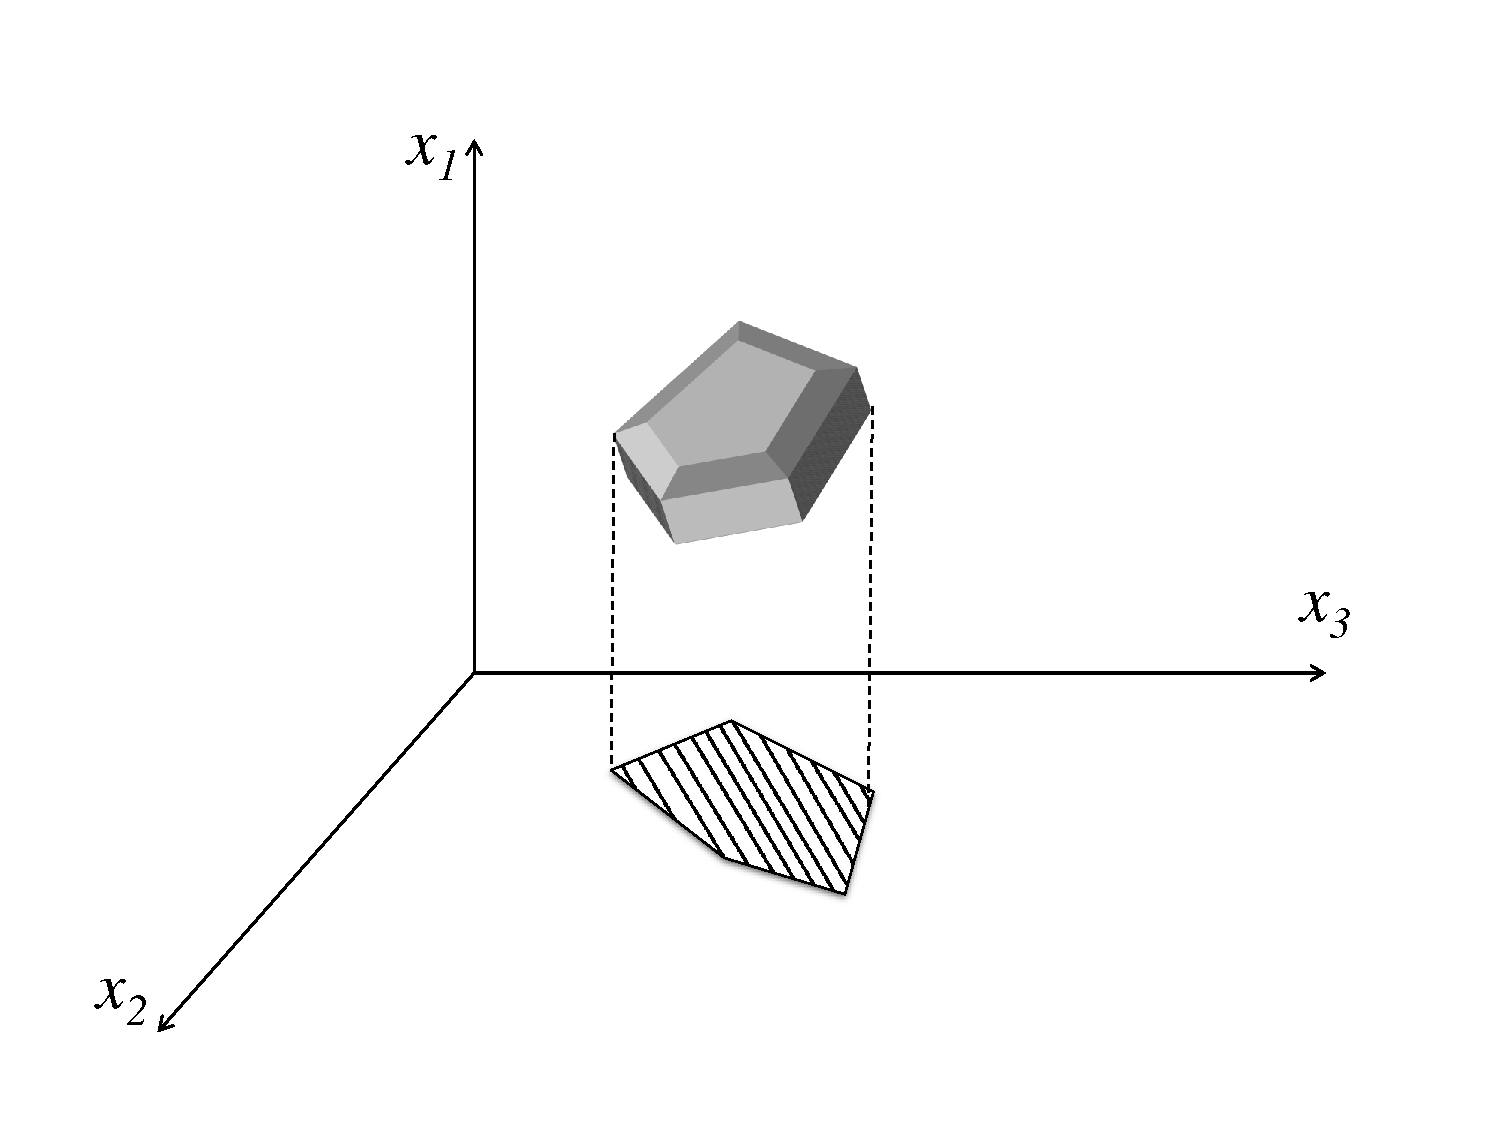
\includegraphics[scale=0.25]{../newfig/projection.pdf}
\end{figure}
\end{column}
\begin{column}{0.5\textwidth}
\begin{figure}
\centering
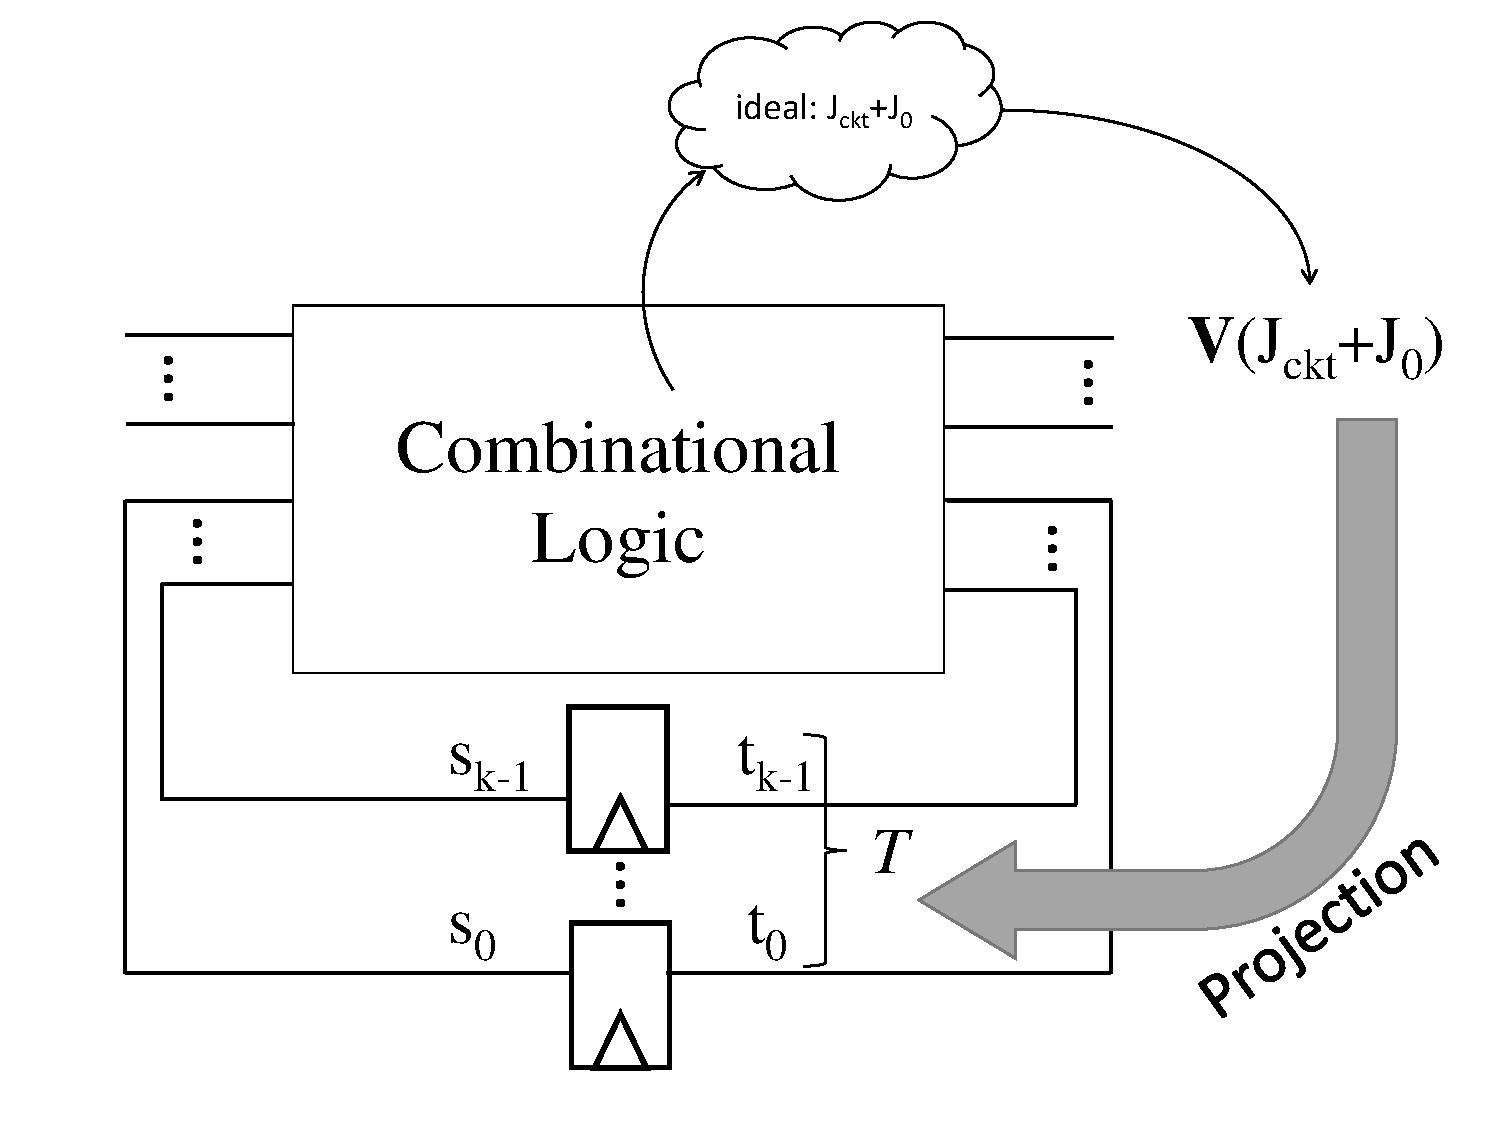
\includegraphics[scale=0.25]{../newfig/proj_reacha.pdf}
\end{figure}
\end{column}
\end{columns}
\bi
\item Projection of variety from $\F[x_1,x_2,x_3]$ to $\F[x_2,x_3]$
\item Projection of ckt ideal's variety on next state (NS) variables $T$
\pause
\item GB($J_{ckt}+J_0$)$\cap\F_2[T] \implies $Next state polynomial $f(T)$!
\ei
\end{frame}
%%%%%%%%%%%%%%%%%%%%%%%%%%%%%%%%%%%%%%%%%%%%%%%%%%%%%%%%%%%%%%%
\begin{frame}{\large{BFS traversal algorithm}}
\begin{algorithm}[H]
\SetAlgoNoLine
 \KwIn{Transition functions $\Delta$, initial state $S^0$}
  $from^0 = reached = S^0$\;
  \Repeat{$new^i == 0$}
  {
  	$i \gets i + 1$\;
\alert{	$to^i \gets$Img$(\Delta, from^{i-1})$}\;
	$new^i \gets to^i \cap \overline{reached}$\;
  	$reached \gets reached \cup new^i$\;
	$from^i \gets new^i$\;
  }
\Return{$reached$}
\caption {Breadth-first Traversal Algorithm}
\end{algorithm}
\pause
\bi
\item Image function: $\text{Img}(\Delta, from) = \exists _s ~\exists _x ~[ T(s, x, t)
  \land from ] = \exists _s ~\exists _x ~\bigwedge_
  {i=1}^{n} (t_i
\overline{\oplus } \Delta_i)\land from$
\item In $\mathbb B^k$, image function $\Leftrightarrow \exists$
\item In $\mathbb F_{2^k}$, need to implement \alert{quantifier elimination}
\ei
\end{frame}
%%%%%%%%%%%%%%%%%%%%%%%%%(copy 17~24 HLDVT)%%%%%%%%%%%%%%%%%%%%%%%%%%
\begin{frame}{\large{Recall: Breadth-First Traversal Algorithm}}
\only<1>{
\begin{algorithm}[H]
\SetAlgoNoLine
 \KwIn{Transition functions $\Delta$, initial state $S^0$}
  $from^0 = reached = S^0$\;
  \Repeat{$new^i == 0$}
  {
  	$i \gets i + 1$\;
	$to^i \gets$Img$(\Delta, from^{i-1})$\;
	$new^i \gets to^i \cap \overline{reached}$\;
  	$reached \gets reached \cup new^i$\;
	$from^i \gets new^i$\;
  }
\Return{$reached$}
\caption {Breadth-first Traversal Algorithm}
\end{algorithm}

\textbf{Implement this algorithm by finding analogs in algebraic geometry}
}
\only<2>{
\begin{algorithm}[H]
\SetAlgoNoLine
 \KwIn{Transition functions $\Delta$, initial state $S^0$\tcp*{\alert{polynomial ideal}}}
  $from^0 = reached = S^0$\tcp*{\alert{set of states $\Leftrightarrow$ variety of ideal}}
  \Repeat{$new^i == 0$}
  {
  	$i \gets i + 1$\;
	$to^i \gets$Img$(\Delta, from^{i-1})$\;
	$new^i \gets to^i \cap \overline{reached}$\;
  	$reached \gets reached \cup new^i$\;
	$from^i \gets new^i$\;
  }
\Return{$reached$}
\caption {Breadth-first Traversal Algorithm}
\end{algorithm}

\textbf{Implement this algorithm by finding analogs in algebraic geometry}
}
\only<3>{
\begin{algorithm}[H]
\SetAlgoNoLine
 \KwIn{Transition functions $\Delta$, initial state $S^0$\tcp*{\alert{polynomial ideal}}}
  $from^0 = reached = S^0$\tcp*{\alert{set of states $\Leftrightarrow$ variety of ideal}}
  \Repeat{$new^i == 0$}
  {
  	$i \gets i + 1$\;
	$to^i \gets$Img$(\Delta, from^{i-1})$\tcp*{\alert{GB of Elim ideal}}
	$new^i \gets to^i \cap \overline{reached}$\;
  	$reached \gets reached \cup new^i$\;
	$from^i \gets new^i$\;
  }
\Return{$reached$}
\caption {Breadth-first Traversal Algorithm}
\end{algorithm}

\textbf{Implement this algorithm by finding analogs in algebraic geometry}
}
\only<4>{
\begin{algorithm}[H]
\SetAlgoNoLine
 \KwIn{Transition functions $\Delta$, initial state $S^0$\tcp*{\alert{polynomial ideal}}}
  $from^0 = reached = S^0$\tcp*{\alert{set of states $\Leftrightarrow$ variety of ideal}}
  \Repeat{$new^i == 0$}
  {
  	$i \gets i + 1$\;
	$to^i \gets$Img$(\Delta, from^{i-1})$\tcp*{\alert{GB of Elim ideal}}
	$new^i \gets to^i \cap \overline{reached}$\tcp*{\alert{ideal quotient \& sum}}
  	$reached \gets reached \cup new^i$\;
	$from^i \gets new^i$\;
  }
\Return{$reached$}
\caption {Breadth-first Traversal Algorithm}
\end{algorithm}

\textbf{Implement this algorithm by finding analogs in algebraic geometry}
}
\only<5>{
\begin{algorithm}[H]
\SetAlgoNoLine
 \KwIn{Transition functions $\Delta$, initial state $S^0$\tcp*{\alert{polynomial ideal}}}
  $from^0 = reached = S^0$\tcp*{\alert{set of states $\Leftrightarrow$ variety of ideal}}
  \Repeat{$new^i == 0$}
  {
  	$i \gets i + 1$\;
	$to^i \gets$Img$(\Delta, from^{i-1})$\tcp*{\alert{GB of Elim ideal}}
	$new^i \gets to^i \cap \overline{reached}$\tcp*{\alert{ideal quotient \& sum}}
  	$reached \gets reached \cup new^i$\tcp*{\alert{ideal product}}
	$from^i \gets new^i$\;
  }
\Return{$reached$}
\caption {Breadth-first Traversal Algorithm}
\end{algorithm}

\textbf{Implement this algorithm by finding analogs in algebraic geometry}
}
\end{frame}

%%%%%%%%%%%%%%%%%%%%%%%%%%%%%%%%%%%%%%%%%%%%%%%%%%%%%%%%%%%%%%%%%%%%%%%%%
\begin{frame}{\large{Intersection and union in algebraic geometry}}
\begin{Definition}
\label{def:sum}
({\bf Sum/Product of Ideals}) If $I = \langle f_1, \dots, f_r\rangle$ and $J = \langle g_1, \dots, g_s\rangle$ are 
ideals in $\mathbb F[x_1, \dots, x_n]$, then the {\bf sum} of $I$ and $J$ is defined as
$$I + J = \langle f_1, \dots, f_r, g_1, \dots, g_s\rangle$$ And the {\bf product} of $I$ and $J$ is defined
as
\begin{equation}
  I \cdot J = \langle f_ig_j\ |\ 1 \leq i \leq r, 1 \leq j \leq s\rangle \nonumber
  \end{equation}
\end{Definition}
\begin{Theorem}
\label{thm:unionintersect}
If $I$ and $J$ are ideals in $\mathbb F[x_1, \dots, x_n]$, then ${\bf
  V}(I + J) = {\bf V}(I) \bigcap {\bf V}(J)$ and ${\bf V}(I \cdot J) =
{\bf V}(I) \bigcup {\bf V}(J)$. 
\end{Theorem}
\end{frame}

%%%%%%%%%%%%%%%%%%%%%%%%%%%%%%%%%%%%%%%%%%%%%%%%%%%%%%%%%%
\begin{frame}{\large{Complement set in algebraic geometry}}
\begin{Definition}
({\bf Quotient of Ideals}) If $I$ and $J$ are ideals in $\mathbb
  F[x_1, \dots, x_n]$, then $I:J$ is the set
  \begin{equation}
  \{f \in \mathbb F[x_1, \dots, x_n]\ |\ f\cdot g \in I, \forall g \in J\}\nonumber
  \end{equation}
and is called the {\bf ideal quotient} of $I$ by $J$.
\end{Definition}
\begin{Theorem}
\label{thm:quotient}
Let $J_0$ be an ideal of vanishing polynomials over $\Fkk[x_1,\dots,x_n]$, then 
$${\bf V}(J_0:J) = {\bf V}(J_0) - {\bf V}(J) = \overline{{\bf V}(J)}$$
\end{Theorem}
\bi
\item $V(J)\subseteq \Fkk$ in affine space
\item Given ideal $J$, compute $J'$ s.t. $V(J') = \overline{V(J)} = \Fkk-V(J)\implies J'=J_0:J$
\ei
\end{frame}

%%%%%%%%%%%%%%%%%%%%%%%%%%%%%%%%%%%%%%%%%%%%%%%%%%%%%%%%%%%%
\begin{frame}{\large{Our proposed algorithm of BFS traversal based on algebraic geometry}}

\IncMargin{1em}
\begin{algorithm}[H]
\SetAlgoNoLine
\Indm
 \KwIn{The circuit's characteristic polynomial ideal $J_{ckt}$,
   initial state polynomial $\Func(S)$, and LEX term order: bit-level
   variables $x, s, t$ $>$ PS word $S$ $>$ NS word $T$}
\Indp

  $from^0 = reached = \Func(S)$\;
  \Repeat{$\langle new^i\rangle == \langle 1\rangle$}
  {
  	$i \gets i + 1$\;
  	$G \gets$GB($\langle J_{ckt},J_0, from^{i-1}\rangle$)\tcp*{This step contains bit-level}
%  	\tcc{Compute Gr\"obner basis with elimination term order: $T$ smallest}
	$\langle to^i\rangle \gets G\cap \Fkk[T]$\tcp*{Only word-level $S,T$ onwards}
%	\tcc{There will be a univariate polynomial in $G$ denoting the
%          set of next states in word-level variable $T$}
	$\langle new^i\rangle \gets \langle to^i\rangle + (\langle T^{2^k}-T\rangle:\langle reached\rangle)$\;
%	\tcc{Use quotient of ideals to attain complement of reached states, then use sum of ideals to attain an intersection with next state}
  	$\langle reached\rangle \gets \langle reached\rangle \cdot \langle new^i\rangle$\;
%  	\tcc{Use product of ideals to attain a union of newly reached states and formerly reached states}
	$from^i \gets new^i(S\setminus T)$\;
%	\tcc{Start a new iteration by replacing variable $T$ in newly reached states with current state variable $S$}
  }
%  \tcc{Loop until a fixpoint reached: newly reached state is empty}
\Return{$\langle reached\rangle$}
\caption {Algebraic Geometry based FSM Traversal}
\end{algorithm}
\DecMargin{1em}

\hyperlink{pptpage2}{\beamergotobutton{Go to example page 2}}
\end{frame}

%%%%%%%%%%%%%%%%%%%%%%%%%%%%%%%%%%%%%%%%%%%%%%%%%%%%%%%%%%%%
\begin{frame}{\large{Full Blown traversal of example circuit using algebraic geometry}}
\bi
\item Initial state $from^0 = S(\{00\})$
\item {\bf Iteration 1:}Compose an elimination ideal $J$ 
\ei
\vspace{-0.2in}
\begin{columns}[onlytextwidth]
\begin{column}{0.5\textwidth}
\begin{align*}
&f_1: t_0- (xs_0s_1+xs_0\\
&+xs_1+x+s_0+s_1+1)\\
&f_2: t_1 - (xs_0+x+s_0s_1+s_0)\\
&f_3: S - s_0 - s_1\alpha\\
&f_4: T - t_0 - t_1\alpha
\end{align*}
\end{column}
\vspace{-0.2in}
\begin{column}{0.5\textwidth}
\begin{align*}
&f_5: x^2-x\\
&f_6: s_0^2-s_0, f_7: s_1^2-s_1\\
&f_8: t_0^2-t_0, f_9: t_1^2-t_1\\
&f_{10}: S^4-S, f_{11}:T^4-T
\end{align*}
\end{column}
\end{columns}
\begin{columns}[onlytextwidth]
\begin{column}{0.7\textwidth}
\begin{figure}[H]
\centering{
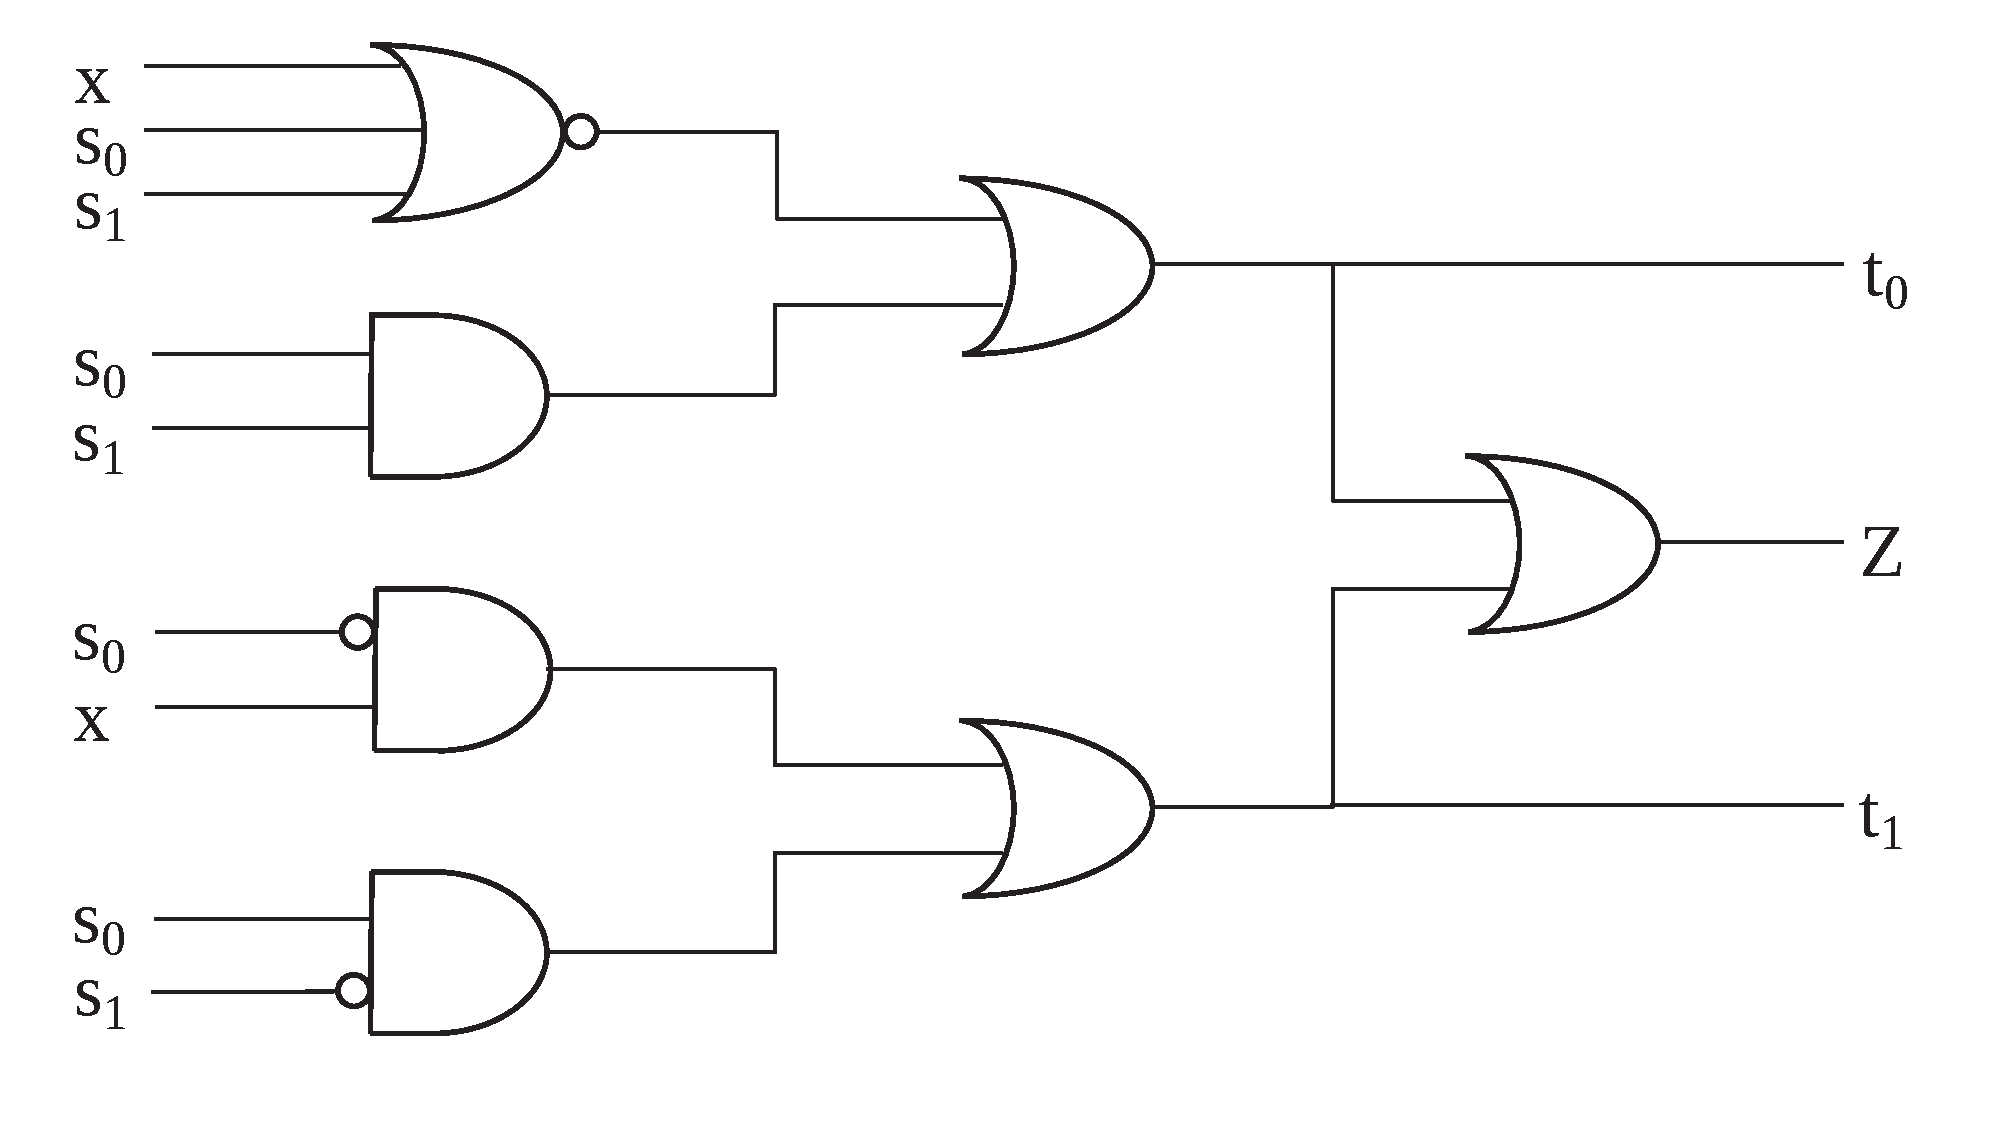
\includegraphics[width=3in]{hehe.pdf}
}
\end{figure}
\end{column}
\begin{column}{0.3\textwidth}
$J_{ckt} = \langle f_1,f_2,f_3,f_4\rangle$\\
$J_0 = \langle f_5,f_6,\dots,f_{11}\rangle$
\end{column}
\end{columns}
\end{frame}
%%%%%%%%%%%%%%%%%%%%%%%%%%%%%%%%%%%%%%%%%%%%%%%%%%%%%%%%%%%
\begin{frame}[label = pptpage2]{\large{Full Blown traversal of example circuit using algebraic geometry}}
\bi
\item Elimination term order: 
$$\{x,s_0,s_1,t_0,t_1\}~(all~bits)~>~S~(PS~word)~ >~ T~(NS~word)$$
\item Compute the reduced GB for $J = J_{ckt}+J_0+\langle from^0\rangle$
\item Next state 
$$to^1 = \langle T^2+(\alpha+1)T+\alpha\rangle$$ 
\item Mapping to set of states
$$V(to^1) = \{1,\alpha\} \Leftrightarrow \{01,10\}$$
\item Complement of formerly reached state:
$$\langle T^4-T\rangle:\langle T\rangle = \langle T^3+1\rangle$$ 
\item Mapping to set of states
$$V(\langle T^3+1\rangle) = \{1,\alpha,1+\alpha\} \Leftrightarrow \{01,10,11\}$$
\ei
\hyperlink{linkSTG}{\beamergotobutton{STG}}
\end{frame}
%%%%%%%%%%%%%%%%%%%%%%%%%%%%%%%%%%%%%%%%%%%%%%%%%%%%%%%%%%%
\begin{frame}[label = pptpage3]{\large{Full Blown traversal of example circuit using algebraic geometry}}
\bi
\item Newly reached states:
$$\langle T^3+1, T^2+(\alpha+1)T+\alpha \rangle = \langle T^2+(\alpha+1)T+\alpha \rangle~(\{01,10\})$$ 
\item Update current reached states 
$$reach = \langle T\cdot T^2+(\alpha+1)T+\alpha \rangle = \langle T^3+(\alpha+1)T^2+\alpha T\rangle$$ 
\item Mapping to set of states
$$V(reached) = \{0,1,\alpha\} \Leftrightarrow \{00,01,10\}$$
\item Update the present states for next iteration
$$from^1 = \langle S^2+(\alpha+1)S+\alpha\rangle$$
\ei
\hyperlink{linkSTG}{\beamergotobutton{STG}}
\end{frame}


%%%%%%%%%%%%%%%%%%%%%%%%%%%%%%%%%%%%%%%%%%%%%%%%%%%%%%%%%%%
\begin{frame}{\large{Full Blown traversal of example circuit using algebraic geometry}}
\bi
\item Iteration 2:
	\bi
	\item Next state: $to^2 = \langle T^2+\alpha T\rangle~(\{00,10\})$
	\item The complement of $reached$:
	$$\langle T^4-T\rangle:\langle T^3+(\alpha+1)T^2+\alpha T\rangle
= \langle T + 1+\alpha\rangle ~(\{11\})$$ 
	\item Newly reached state: 
$$\langle T^2+\alpha T, T+1+\alpha \rangle = \langle \alert{1}\rangle$$ 
	\ei
\item Algorithm terminates
\item Return value (final reachable states):
$$reached = \langle T^3+(\alpha+1)T^2+\alpha T\rangle$$
\ei
\end{frame}

%%%%%%%%%%%%%%%%%%%%%%%%%%(End of copy)%%%%%%%%%%%%%%%%%%%%%%%%%%%%%%
\begin{frame}{\large{Improve complexity using RATO [Pruss, '15]}}
\bi
\item Directly compute GB($J_{ckt}+J_0$) in $\Fq$ is costly ($q^{O(n)}$)
\item GB sensitive to term order$\to$Transform to simpler set for GB?
\pause
\item RATO: reverse topological traverse on ckt structure
\ei
\begin{figure}[H]
\centering{
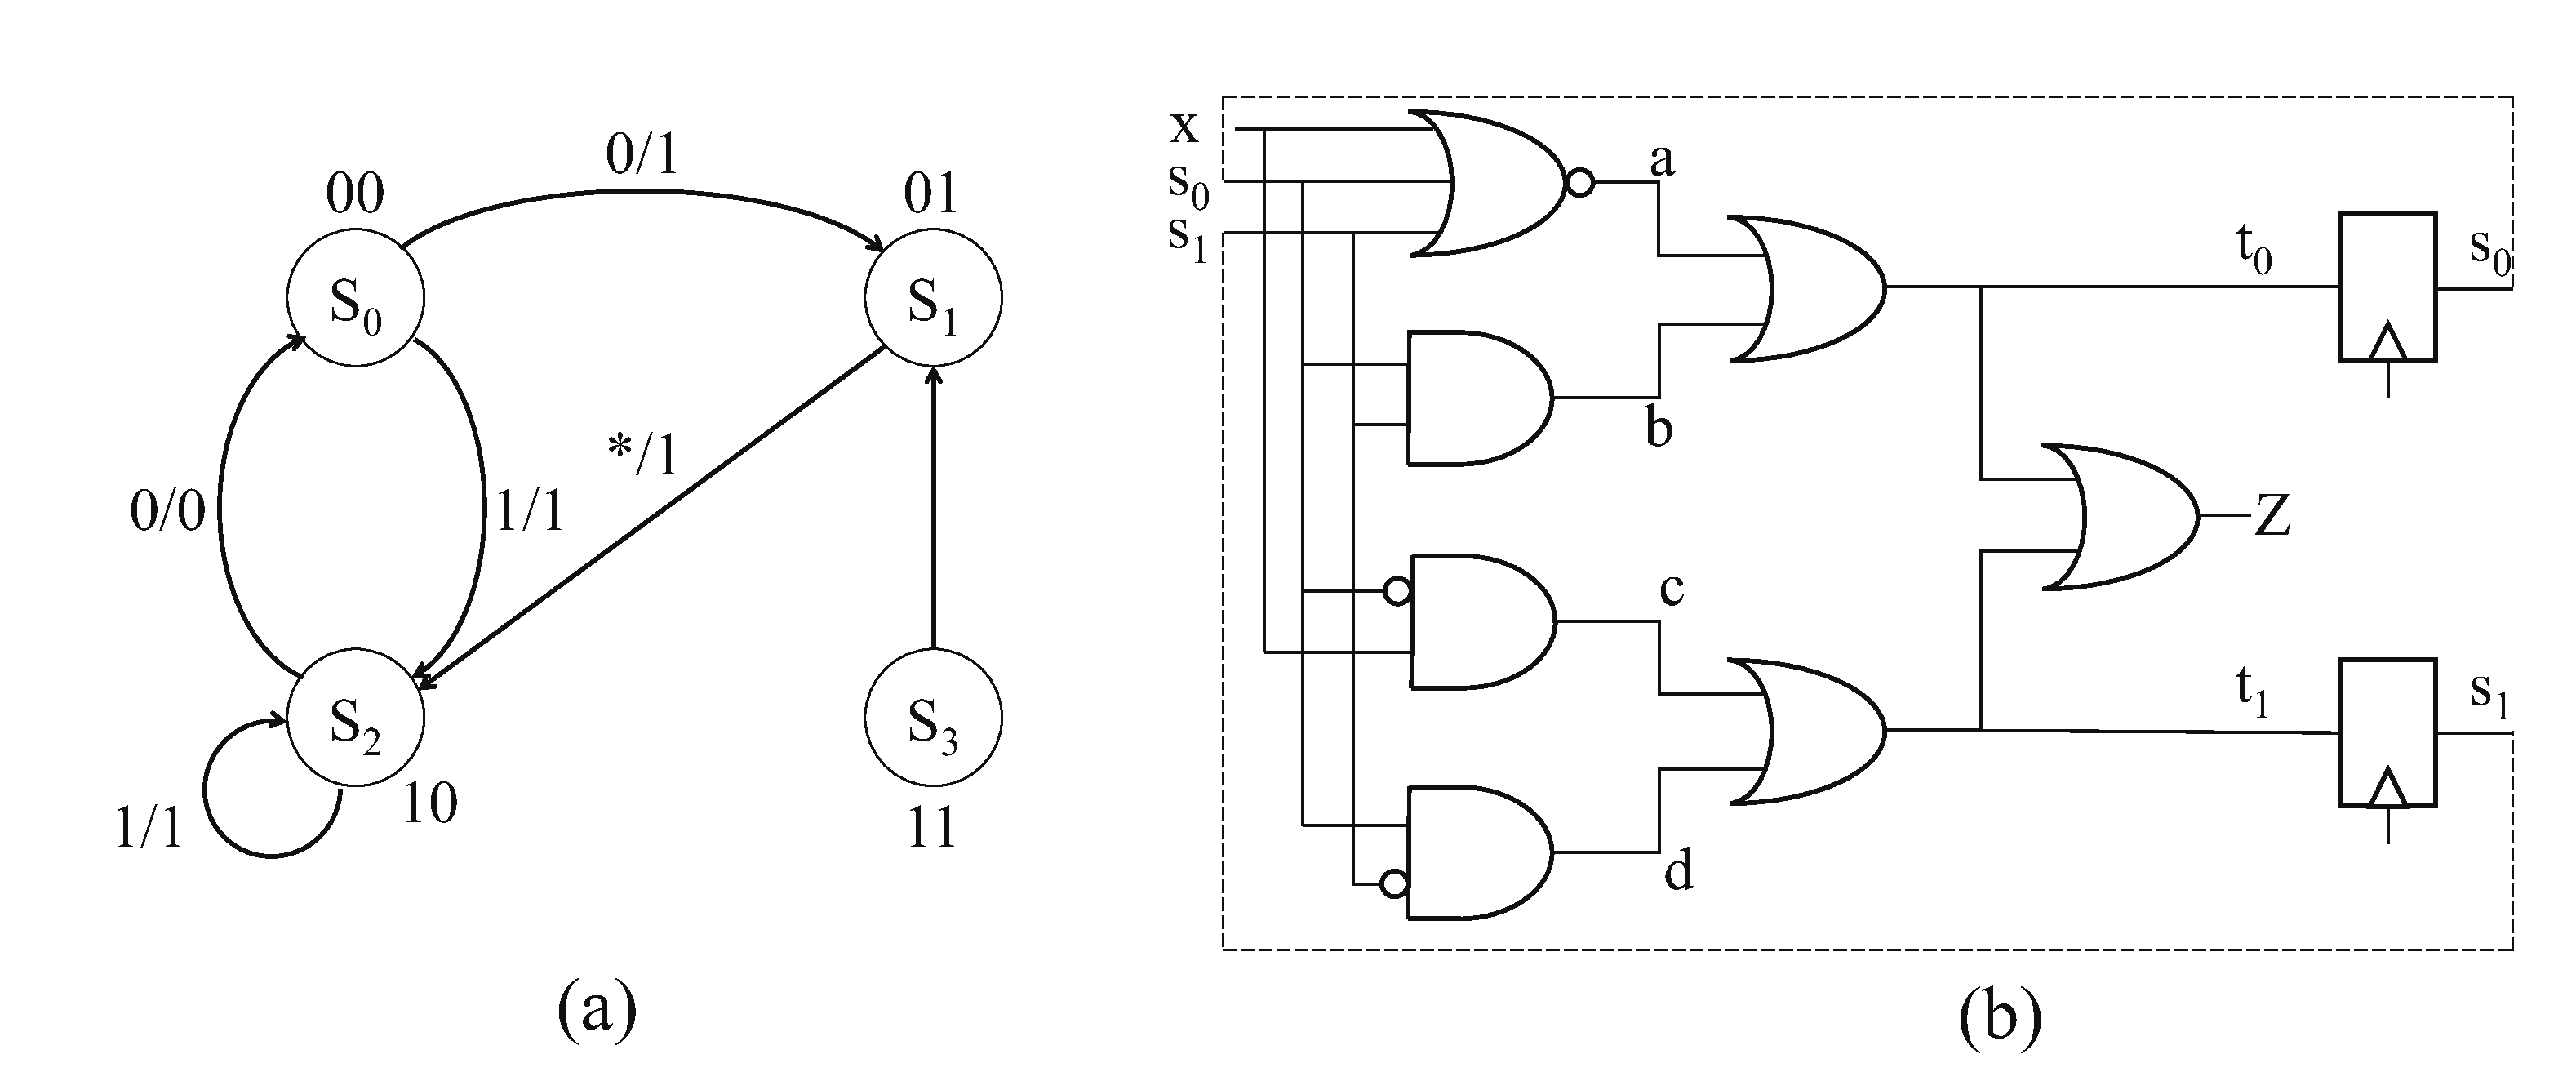
\includegraphics[width=4.5in]{../newfig/new_stg.eps}
\label{fig:fsm}}
\end{figure}

\end{frame}
%%%%%%%%%%%%%%%%%%%%%%%%%%%%%%%%%%%%%%%%%%%%%%%%%%%%%%%%%%%%%%%%%%
\begin{frame}[label = linkRATO]{\large{Benefits of using RATO}}
\bi
\item Definition of RATO:\par 
``bit-level variables ordered reverse topologically "$ > T>S$
\item Topology in ckt structure
	\bi
	\item Output of each gate $= lt(f_i)$
	\ei
\item Product criterion: $gcd(lt(f_i),lt(f_j)) = 1 \implies Spoly(f_i,f_j) \xrightarrow{J_{ckt}+J_0}_+ 0$
\hyperlink{Buch}{\beamergotobutton{Buchberger}}
\item Only one pair of poly with non-relatively-prime leading terms
	
\item $Spoly$ division
	\bi
	\item Divide with levelization
	\item Only inputs (primary \& pseudo) left!
	\ei
\ei
\end{frame}
%%%%%%%%%%%%%%%%%%%%%%%%%%%%%%%%%%%%%%%%%%%%%%%%%%%%%%%%%%%%%
\begin{frame}{\large{Example of using RATO}}
\bi
\item RATO: LEX with $(t_0,t_1)>(a,b,c,d)>(x,s_0,s_1)>T>S$
\ei
\begin{equation*}
f_1: a+xs_0s_1+xs_0+xs_1+x+s_0s_1+s_0+s_1+1
\end{equation*}
\vspace{-0.8cm}
\begin{alignat*}{2}
f_2: b+s_0s_1 &~~~ f_3: c+x+xs_0 &&~~~f_4: d+s_0s_1+s_0 \\
f_5: \alert{t_0}+ab+a+1 &~~~ f_6: t_1+cd+c+d &&~~~ f_7: \alert{t_0}+t_1\alpha+T 
\end{alignat*}
\bi
\item $Spoly$ reduction gives $T+\Func(primary/pseudo~inputs)$
\ei
\begin{align}
&Spoly(f_5,f_7) \xrightarrow{J_{ckt}+J_0}_{+}T + s_0 s_1 x+\alpha s_0 s_1 \nonumber\\
&+(1+\alpha)s_0 x+(1+\alpha) s_0+s_1 x+s_1+(1+\alpha) x+1\nonumber
\end{align}
\bi
\item {\bf Q:} How to get rid of bit-level inputs?
\ei
\end{frame}
%%%%%%%%%%%%%%%%%%%%%%%%%%%%%%%%%%%%%%%%%%%%%%%%%%%%%%%%%%%
\begin{frame}{\large{Bit-to-word conversion}}
\bi
\item Objective: find $s_i = \mathcal G(S)$
\item $(s_0+s_1\alpha+\cdots+s_{k-1}\alpha^{k-1})^{2^n} = s_0^{2^n}+(s_1\alpha)^{2^n}+\cdots+(s_{k-1}\alpha^{k-1})^{2^n}$
\item Build system of poly eqns by squaring poly:\\
$S = s_0+s_1\alpha+\cdots+s_{k-1}\alpha^{2^{k-1}}$
\begin{align*}
\label{eqn:alphamat}
\begin{bmatrix}
S \\
S^2 \\
S^{2^2} \\
\vdots \\
S^{2^{k-1}}
\end{bmatrix}
&=
\begin{bmatrix}
1 & \alpha & \alpha^{2} & \cdots & \alpha^{{k-1}}\\
1 & \alpha^{2} & \alpha^{4} & \cdots & \alpha^{2(k-1)} \\
1 & \alpha^{4} & \alpha^{8} & \cdots & \alpha^{4(k-1)}\\
\vdots & \vdots & \vdots & \ddots & \vdots \\
1 & \alpha^{2^{k-1}} & \alpha^{2\cdot 2^{k-1}} & \cdots & \alpha^{(k-1)\cdot 2^{k-1}}
\end{bmatrix}
\begin{bmatrix}
s_0\\
s_1\\
s_2\\
\vdots\\
s_{k-1}
\end{bmatrix}
\end{align*}
\item Transition function $f_T: T+\Func(S,x)$
\item Elimination on ideal $\langle f_T,f_S \rangle+J_0$ using $S,x > T$
\ei
\end{frame}
%%%%%%%%%%%%%%%%%%%%%%%%%%%%%%%%%%%%%%%%%%%%%%%%%%%%%%%%
\begin{frame}{\large{FSM traversal algorithm with RATO}}
\IncMargin{1em}
\begin{algorithm}[H]
\SetAlgoNoLine
\LinesNumbered
\Indm
 \KwIn{Polynomial ideal $J_{ckt}$, initial state polynomial $\Func(S)$}
 \KwOut{Final reachable states represented by polynomial $\mathcal G(T)$}
\Indp

  $from^0 = reached = \Func(S)$\;
  $f_T = $Reduce($Spoly(f_w,f_g), J_{ckt})$\;
  \tcc{Compute $Spoly$ for the critical pair, then reduce it with circuit ideal under RATO}
	Eliminate bit-level variables in $f_T$\;
  \Repeat{$\langle new^i\rangle == \langle 1\rangle$}
  {
  	$i \gets i + 1$\;
  	$G \gets$GB($\langle f_T , from^{i-1}\rangle+J_0^{PI}$)\;
%  	\tcc{Compute Gr\"obner basis with elimination term order: $T$ smallest; $J_0^{PI}$ covers all possible inputs from PIs}
	$to^i \gets G\cup \Fkk[T]$\;
%	\tcc{There will be a univariate polynomial in $G$ denoting next state in word-level variable $T$}
	$\langle new^i\rangle \gets \langle to^i\rangle + (\langle T^{2^k}-T\rangle:\langle reached\rangle)$\;
%	\tcc{Use quotient of ideals to attain complement of reached states, then use sum of ideals to attain an intersection with next state}
  	$\langle reached\rangle \gets \langle reached\rangle \cdot \langle new^i\rangle$\;
%  	\tcc{Use product of ideals to attain a union of new reached states and formerly reached states}
	$from^i \gets new^i(S\setminus T)$\;
%	\tcc{Start a new iteration by replacing variable $T$ in new reached states with current state variable $S$}
  }
%  \tcc{Loop until a fix-point reached: newly reached state is empty}
\Return{$\langle reached\rangle$}
\caption {Refined Algebraic Geometry based FSM Traversal}\label{alg:refined}
\end{algorithm}
\DecMargin{1em}

\end{frame}
%%%%%%%%%%%%%%%%%%%%%%%%%%%%%%%%%%%%%%%%%%%%%%%%%%%%%%%%
\begin{frame}{\large{Experiment results: word-level traversal}}
\begin{table}[H]
\centering
\caption{Results of running benchmarks using our tool. 
\small{Parts I to III denote the time taken by polynomial divisions,
  bit-level to word-level abstraction and iterative reachability
  convergence checking part of our approach, respectively.}}
{\small 
\begin{tabular}{|c||c|c|c|c|c|c|}
\hline
\multirow{3}{*}{\centering Benchmark} 
 & \multirow{3}{0.9cm}{\centering \# States}
 & \multirow{3}{1.3cm}{\centering \# iterations}
 & \multicolumn{3}{c|}{\multirow{2}{2.0cm}{\centering Runtime (sec)}}
 & \multirow{3}{1.8cm}{\centering Runtime of VIS (sec)} \\
   & & &\multicolumn{3}{c|}{}& \\
  \cline{4-6}
     & & & I & II & III & \\
\hline
\hline
b01 & 18  & 5  & $<0.01$ & 0.01 & 0.02 & $<0.01$\\
b02 & 8 & 5 & $<0.01$  & 0.01 & $<0.01$ & $<0.01$ \\
b06 & 13 & 4 & $<0.01$ & 0.07 & 5.0 & $<0.01$ \\
s27 & 6 & 2 & $<0.01$ & 0.01 & 0.02  & $<0.01$  \\
s208 & 16 & 16 & $<0.01$ & 0.32 & 2.4 & $<0.01$ \\
s386 & 13  & 3 & 1.0 & 7.6 & 8.2  & $<0.01$ \\
bbara & 10 & 6 & 0.04 & 0.01 & 0.04  & $<0.01$ \\
beecount & 7  & 3  &$<0.01$ & 0.01 & 0.01 & $<0.01$ \\
dk14 & 7  & 2  & 45 & $<0.01$ & 0.08 & $<0.01$\\
donfile & 24 & 3  & 12316 & 0.02 & 1.7  & $<0.01$\\
\hline
\end{tabular}
}
\label{tab:result}  
\end{table} 
\end{frame}
%%%%%%%%%%%%%%%%%%%%%%%%%%%%%%%%%%%%%%%%%%%%%%%%%%%%%%
\begin{frame}[label = Moore]{\large{Apply FSM traversal to arithmetic ckts}}
\vspace{-0.1in}
\begin{figure}[hbt]
\centering{
%\begin{minipage}{12cm}
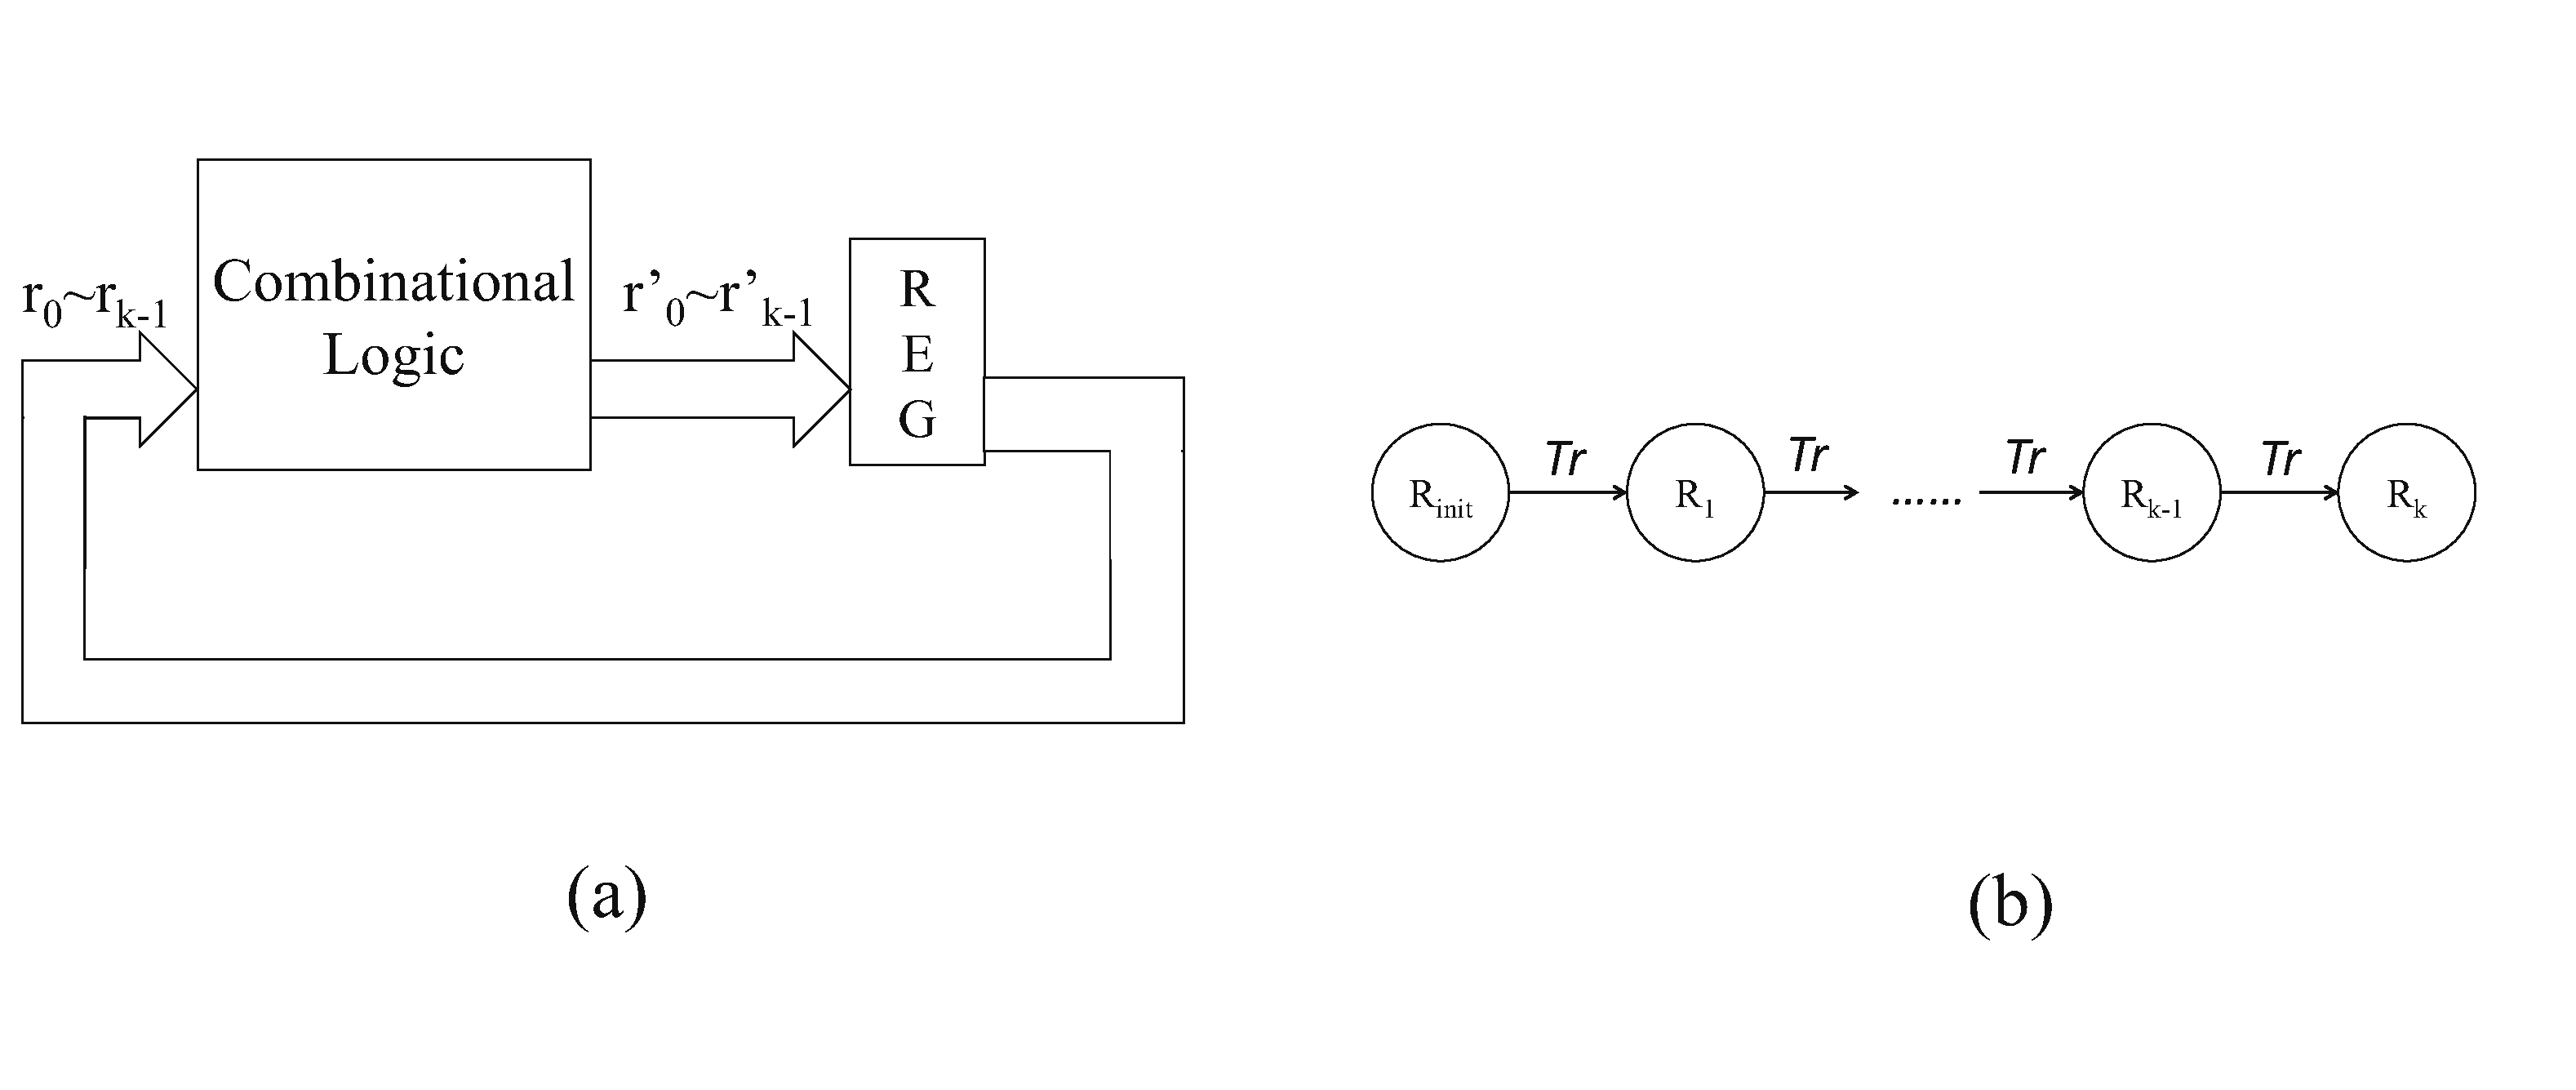
\includegraphics[width=4.5in]{../newfig/Moore.eps}
% \vspace{-0.2in}
%\caption{A simple Moore FSM and its state transition graph}
%\end{minipage}
\label{fig:Moore}}
\end{figure}
\vspace{-0.4in}
\bi
\item Model: restricted Moore finite state machine
	\bi
	\item Some sequential arithmetic circuits will give results after running for $k$ clock cycles
	\item The initial operands are preloaded in register files
	\ei
\item State transitions on this model:
$$R_{k} = Tr(R_{k-1}) = Tr(Tr(\cdots Tr(R_{init})\cdots)) = Tr^k(R_{init})$$
\item Word-level unrolling
\ei
\hyperlink{motiv2}{\beamergotobutton{Recall unrolling}}
\end{frame}
%%%%%%%%%%%%%%%%%%%%%%%%%%%%%%%%%%%%%%%%%%%%%%%%%%%%%
\begin{frame}{\large{Galois field multiplier}}
SPEC: $R = A_{init}\cdot B_{init} \pmod {P(\alpha)}$ after $k$ clock cycles
\hspace{-0.3in}\begin{figure}[hbt]
\centering{
%\begin{minipage}{12cm}
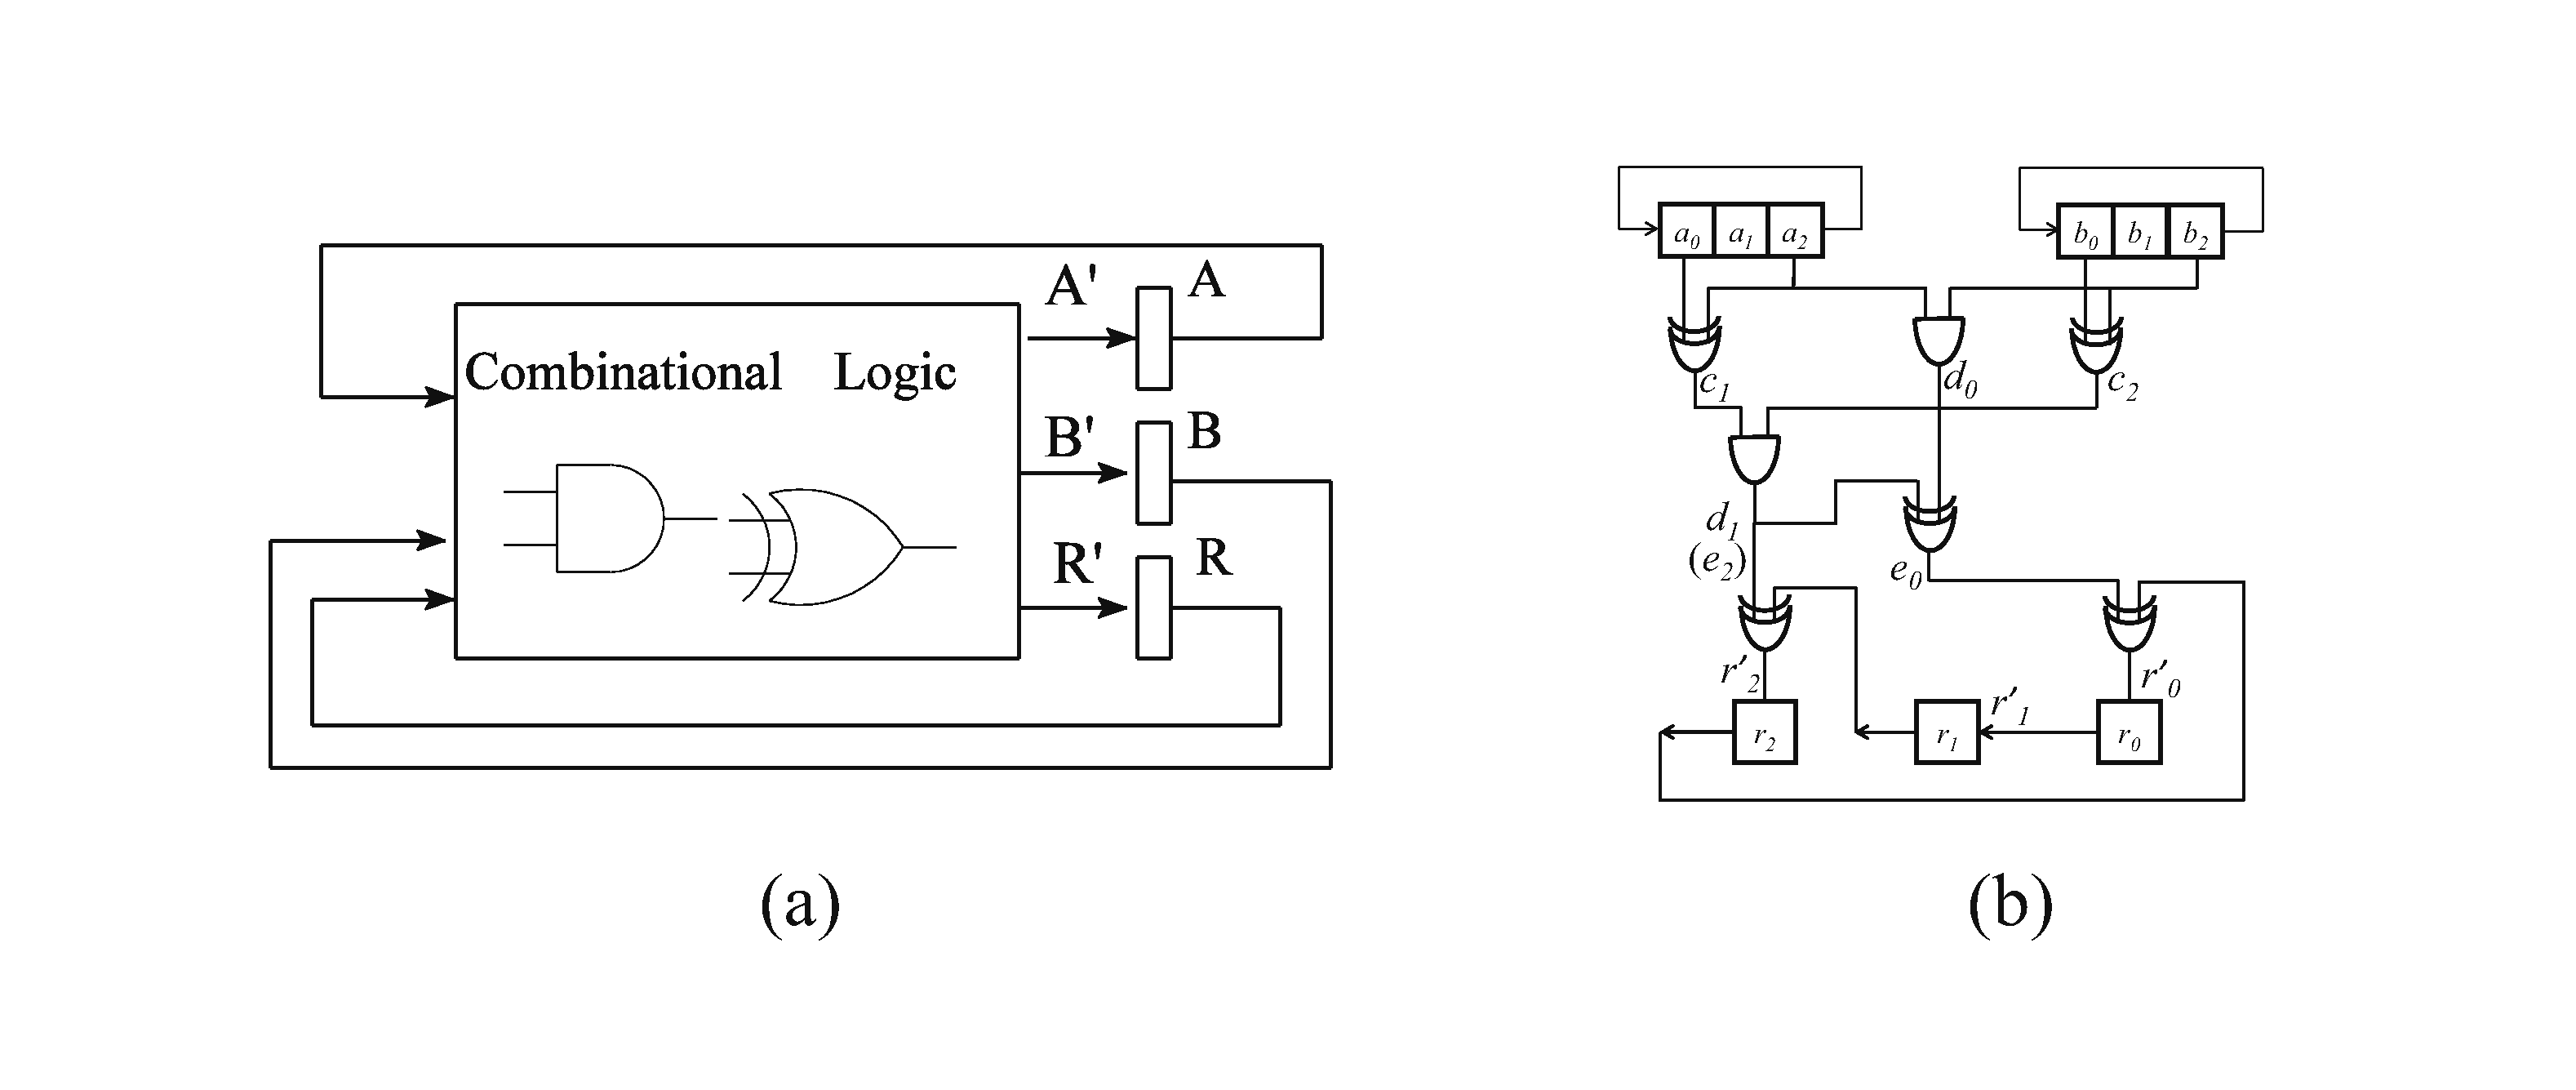
\includegraphics[width=5in]{./new_multi.eps}
%\end{minipage}
\label{fig:RHmulti}}
\end{figure}
\bi
\item Projection on NS $R',A',B'$
\ei
\end{frame}
%%%%%%%%%%%%%%%%%%%%%%%%%%%%%%%%%%%%%%%%%%%%%%%%%%
\begin{frame}{\large{GF multiplier verification algorithm}}
\begin{algorithm}[H] % note [hbt] will fail in beamer
\SetAlgoNoLine
 \KwIn{Circuit polynomial ideal $J$, vanishing ideal $J_0$, initial state ideal $R (=0), \mathcal{G}(A_{init}), \mathcal{H}(B_{init})$} 

  $from_0(R,A,B) = \langle R, \mathcal{G}(A_{init}), \mathcal{H}(B_{init})\rangle$\;
  $i = 0$\;
  \Repeat{$i == k$}
  {
  	$i \gets i + 1$\;
	\alert{$G \gets$GB$( \langle J + J_0+ from_{i-1}(R,A,B) \rangle)$ with ATO}\;
	$to_i(R',A',B')\gets G\cap \mathbb F_{2^k}[R',A',B',R,A,B]$\;
	$from_i \gets to_i(\{R,A,B\}\setminus \{R',A',B'\})$\;
  }
\Return{$from_k(R_{final})$}
\caption {Abstraction via implicit unrolling for Sequential GF circuit verification}
\end{algorithm}
\end{frame}
%%%%%%%%%%%%%%%%%%%%%(copy from DATE18~21)%%%%%%%%%%%%%%%%%%%%%%%%%%
\begin{frame}{\large{Experiment on 3-bit RH-SMPO}}
\begin{figure}[hbt]
\centering{
%\begin{minipage}{12cm}
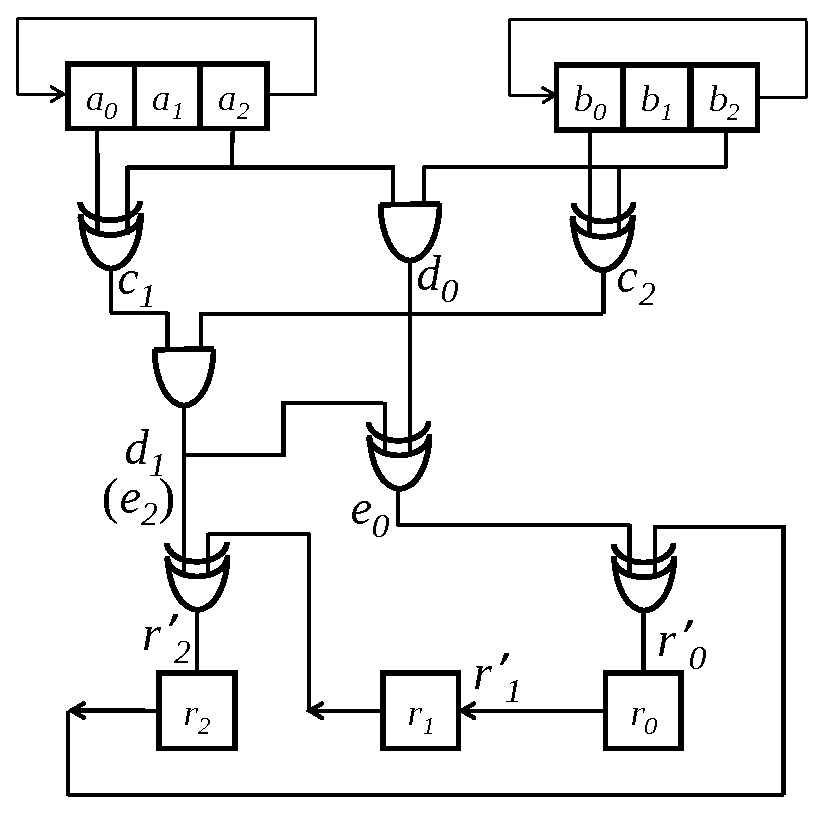
\includegraphics[width=1.5in]{./RH3.eps}
% \vspace{-0.2in}
%\caption{Gate-level circuit of 3-bit RH-SMPO}
%\end{minipage}
\label{fig:RHmulti}}
\end{figure}
\vspace{-0.2in}
\bi
\item The elimination ideal (first iteration):
\begin{align*}
J = &d_0+b_2\cdot a_2,
c_1+a_0+a_2,
c_2+b_0+b_2,
d_1+c_1\cdot c_2,\\
&e_0+d_0+d_1,
e_2+d_1,
r_0'+r_2+e_0,
r_1'+r_0,
r_2'+r_1+e_2,\\
&A+a_0\beta+a_1\beta^2+a_2\beta^4,
B+b_0\beta+b_1\beta^2+b_2\beta^4,\\
&R+r_0\beta+r_1\beta^2+r_2\beta^4,
R'+r_0'\beta+r_1'\beta^2+r_2'\beta^4;
\end{align*}
\ei
\end{frame}
%%%%%%%%%%%%%%%%%%%%%%%%%%%%%%%%%%%%%%%%%%%%%%%%%%%%%%%%%%%
\begin{frame}{\large{Experiment on 3-bit RH-SMPO(2)}}
\bi
\vspace{-3.45cm}
\item $J_0 = \langle x_i^2 - x_i, X^q - X\rangle$
\item $from_0 = \{R, A_{init}+a_0\beta+a_1\beta^2+a_2\beta^4,
B_{init}+b_0\beta+b_1\beta^2+b_2\beta^4\}$
\ei
\end{frame}
%%%%%%%%%%%%%%%%%%%%%%%%%%%%%%%%%%%%%%%%%%%%%%%%%%%%%%%%%%%
\begin{frame}{\large{Basic algorithm to verify the function of sequential GF multipliers}}
\begin{algorithm}[H] % note [hbt] will fail in beamer
\SetAlgoNoLine
 \KwIn{Circuit polynomial ideal $J$, vanishing ideal $J_0$, initial state ideal $R (=0), \mathcal{G}(A_{init}), \mathcal{H}(B_{init})$} 

  $from_0(R,A,B) = \langle R, \mathcal{G}(A_{init}), \mathcal{H}(B_{init})\rangle$\;
  $i = 0$\;
  \Repeat{$i == k$}
  {
  	$i \gets i + 1$\;
	$G \gets$GB$( \langle J + J_0+ from_{i-1}(R,A,B) \rangle)$ with ATO\;
	\alert{$to_i(R',A',B')\gets G\cap \mathbb F_{2^k}[R',A',B',R,A,B]$}\;
	\alert{$from_i \gets to_i(\{R,A,B\}\setminus \{R',A',B'\})$}\;
  }
\Return{$from_k(R_{final})$}
\caption {Abstraction via implicit unrolling for Sequential GF circuit verification}
\end{algorithm}
\end{frame}
%%%%%%%%%%%%%%%%%%%%%%%%%%%%%%%%%%%%%%%%%%%%%%%%%%%%%%%%%%%

\begin{frame}{\large{Experiment on 3-bit RH-SMPO(2)}}
\bi
\item $J_0 = \langle x_i^2 - x_i, X^q - X\rangle$
\item $from_0 = \{R, A_{init}+a_0\beta+a_1\beta^2+a_2\beta^4,
B_{init}+b_0\beta+b_1\beta^2+b_2\beta^4\}$ ($\beta = \alpha^3$)
\item $to_1 : 
R'+(\alpha^2) A_{init}^4 B_{init}^4+(\alpha^2+\alpha) A_{init}^4 B_{init}^2+(\alpha^2+\alpha) A_{init}^4 B_{init}+(\alpha^2+\alpha) A_{init}^2 B_{init}^4+(\alpha^2+\alpha+1) A_{init}^2 B_{init}^2+(\alpha^2) A_{init}^2 B_{init}+(\alpha^2+\alpha) A_{init} B_{init}^4+(\alpha^2) A_{init} B_{init}^2
$
\item $from_1 = \{
R'+(\alpha^2) A_{init}^4 B_{init}^4+(\alpha^2+\alpha) A_{init}^4 B_{init}^2+(\alpha^2+\alpha) A_{init}^4 B_{init}+(\alpha^2+\alpha) A_{init}^2 B_{init}^4+(\alpha^2+\alpha+1) A_{init}^2 B_{init}^2+(\alpha^2) A_{init}^2 B_{init}+(\alpha^2+\alpha) A_{init} B_{init}^4+(\alpha^2) A_{init} B_{init}^2
, A_{init}+a_2\alpha^3+a_0\alpha^6+a_1\alpha^{12},
B_{init}+b_2\alpha^3+b_0\alpha^6+b_1\alpha^{12}\}$
\item $\cdots$
\item After 3 iterations: $to_3 = \{ \alert{R'+A_{init}B_{init},}
~A_{init}+a_0'\alpha^3+a_1'\alpha^6+a_2'\alpha^{12},
~B_{init}+b_0'\alpha^3+b_1'\alpha^6+b_2'\alpha^{12}\}$
\ei
\end{frame}
%%%%%%%%%%%%%%%%%%%%%%%%%%%%%%%%%%%%%%%%%%%%%%%%%%%%%%%%%%%
\begin{frame}{\large{Improve using RATO}}
\begin{algorithm}[H] % note [hbt] will fail in beamer
\SetAlgoNoLine
 \KwIn{Circuit polynomial ideal $J$, vanishing ideal $J_0$, initial state ideal $R (=0), \mathcal{G}(A_{init}), \mathcal{H}(B_{init})$} 

  $from_0(R,A,B) = \langle R, \mathcal{G}(A_{init}), \mathcal{H}(B_{init})\rangle$\;
  $i = 0$\;
  \Repeat{$i == k$}
  {
  	$i \gets i + 1$\;
	\alert{$f_o \xrightarrow{J + J_0+ from_{i-1}(R,A,B)}_+ f_r$ under RATO} \;
	\alert{$to_i(R',A',B')\gets f_r(\{R',A',B'\}\setminus\{r_0,\dots,r_{k-1},a_0,\dots,a_{k-1},b_0,\dots,b_{k-1}\}$}\;
	$from_i \gets to_i(\{R,A,B\}\setminus \{R',A',B'\})$\;
  }
\Return{$from_k(R_{final})$}
\caption {Abstraction via implicit unrolling for Sequential GF circuit verification}
\end{algorithm}
\end{frame}
%%%%%%%%%%%%%%%%%%%%%%%%%%%%%%%%%%%%%%%%%%%%%%%%%%%%%%%
\begin{frame}[label = expSMPO]{\large{Experiment result: sequential GF multiplier verification}}
\bi
\item Run-time for verification of bug-free RH-SMPO circuits
  for SAT, ABC and BDD based methods. \emph{TO} = timeout 14 hrs
\begin{table}[H]
\centering
\label{tbl:equiv}
\begin{tabular}{|c||c|c|c|c|} 
\hline
& \multicolumn{4}{|c|}{Word size of the operands $k$-bits}  \\
\hline
Solver & 11 & 18 & 23 & 33 \\
\hline
\hline
Lingeling & 593  & \emph{TO}  & \emph{TO}  & \emph{TO}\\
\hline
\hline
ABC & 6.24 & \emph{TO} & \emph{TO} & \emph{TO}\\
\hline
\hline
BDD & 0.1 & 11.7 & 1002.4 & \emph{TO}  \\
\hline
\end{tabular}
\label{table:satbdd}  
\end{table} 
\item Runtime for verification of bug-free Agnew's and RH-SMPO circuits using our approach
\hspace{-0.3in}\begin{table}[H]
\centering
\label{tab:Cpp}
{\small 
\begin{tabular}{|c|c||c|c|c|c|c|c|}
\hline
\multicolumn{2}{|c||}{\centering Operand size $k$} & 36 & 60 & 81 & 100 & 131 & 162 \\
\hline
\multirow{2}{1cm}{\centering RH-SMPO} & \#Polys & 4716 & 12960 & 21870 & 35600 & 56592 & 92826 \\
\cline{2-8}
 & Runtime & 14.3 & 213.3 & 1343 & 4685 & 26314 & 124194 \\
\hline
\multirow{2}{1cm}{\centering Agnew's SMPO} & \#Polys & 2700 & 7380 & 13356 & 20300 & 34715 & 52974 \\
\cline{2-8}
 & Runtime & 10.2 & 212.0 & 2684 & 4686 & 56568 & 119441 \\
 
 \hline

\end{tabular}
}
\end{table}
\ei
\hyperlink{motiv2}{\beamergotobutton{Recall SEC miter}}
\end{frame}
%%%%%%%%%%%%%%%%%%%%%%%%%%%%%%%%%%%%%%%%%%%%%%%%
\begin{frame}[label = refine]{\large{Abstraction refinement}}
\begin{figure}[hbt]
\centering{
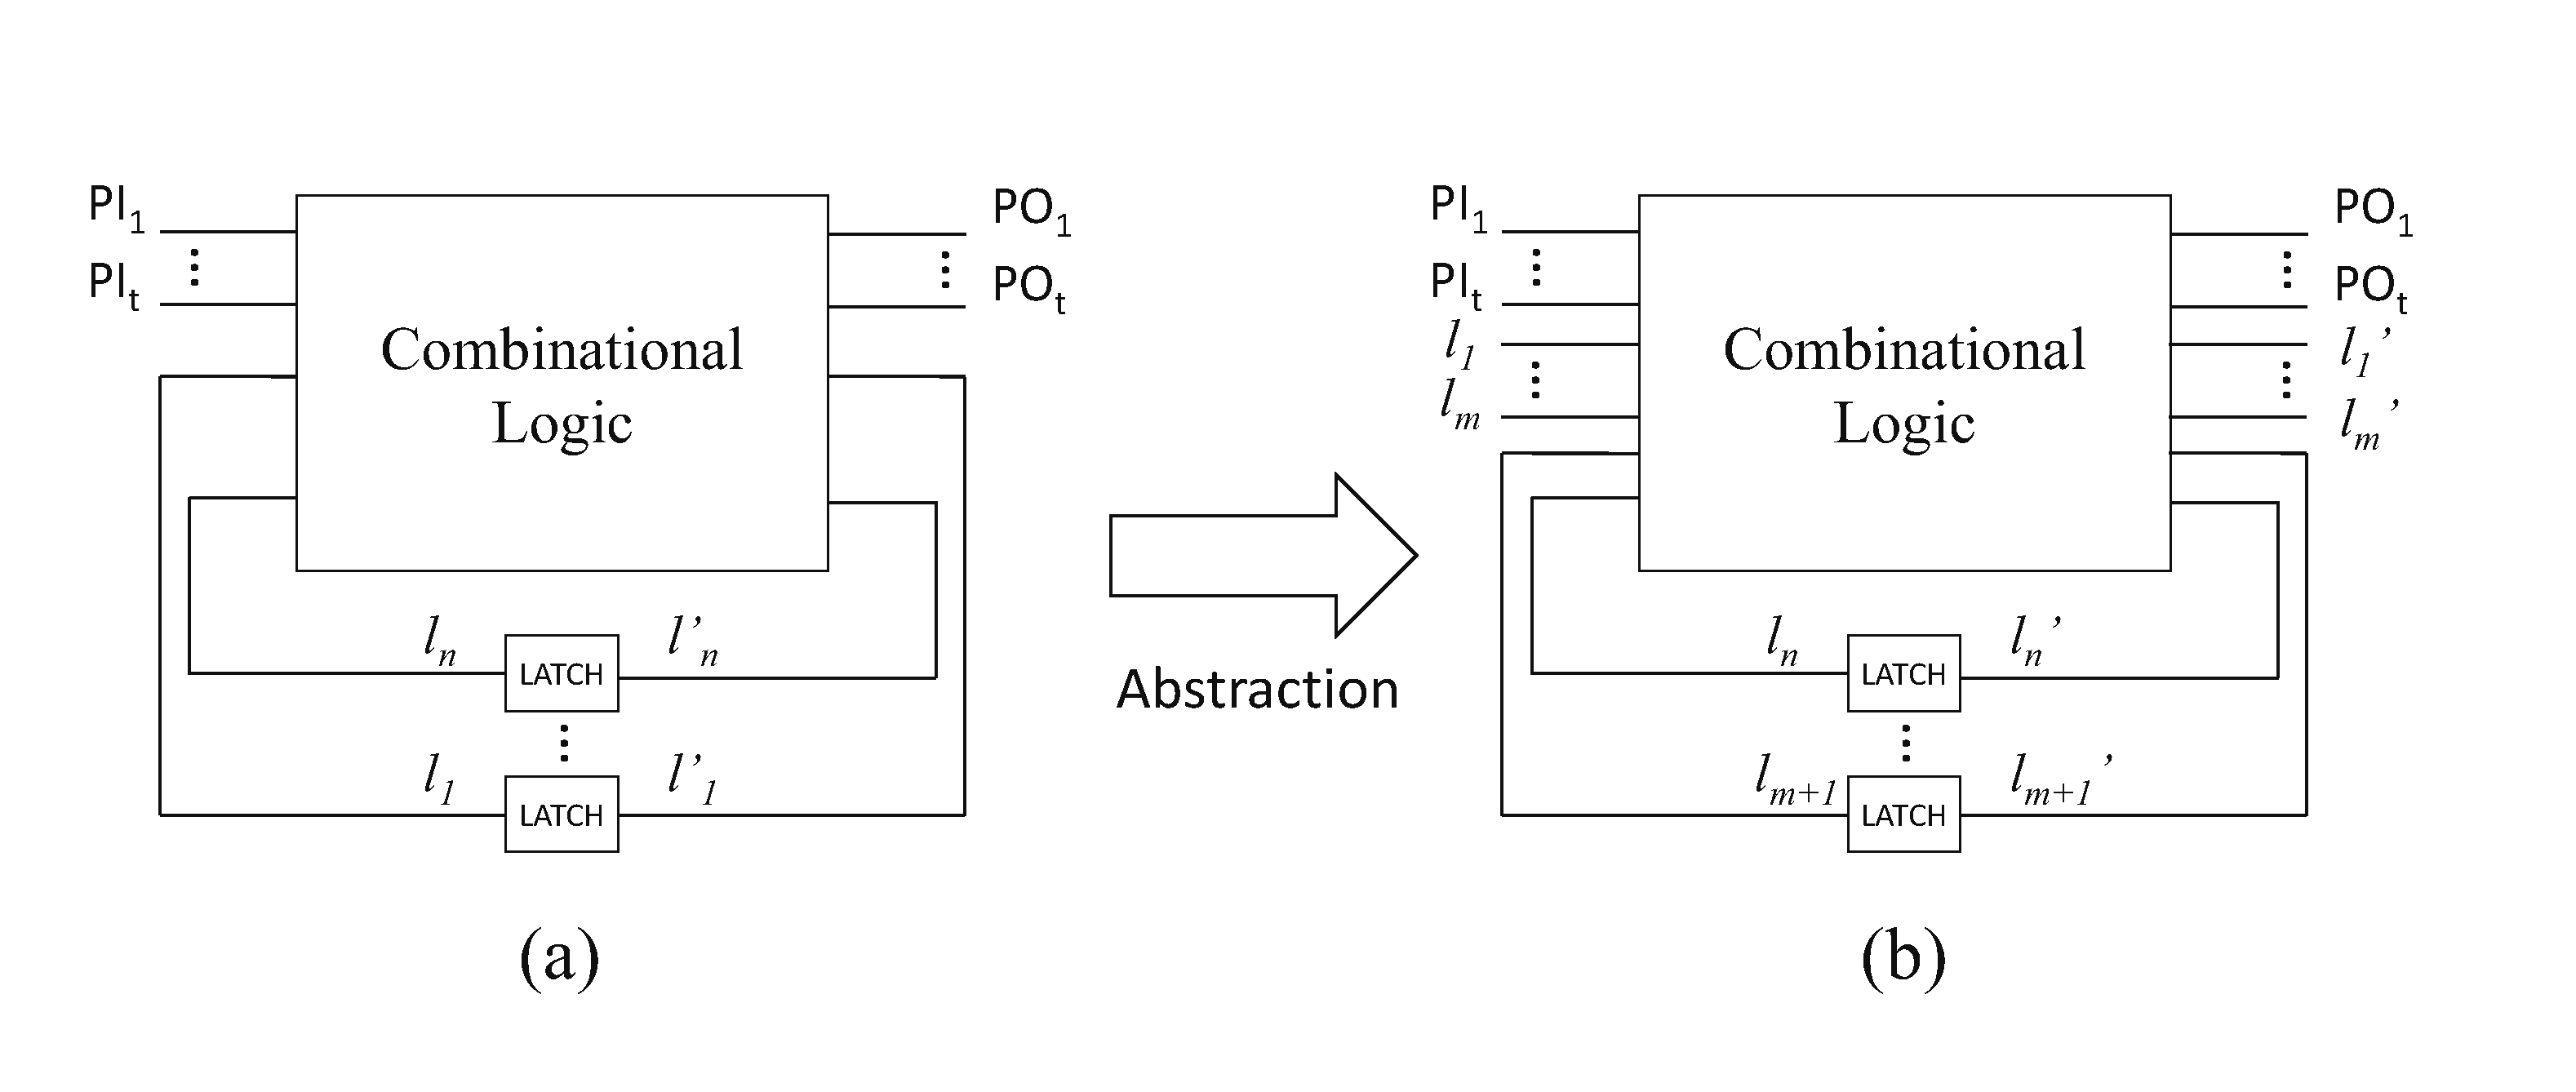
\includegraphics[width=4.5in]{../newfig/refine.eps}
\caption{Abstraction by reducing latches}
\label{fig:refine}}
\end{figure}
\vspace{-0.2in}
\bi
\item Remove ``irrelevant" latches, reduce state space
\item Provide an over-approximation
\item This algorithm requires \alert{UNSAT core extraction}
\ei
\hyperlink{motiv3}{\beamergotobutton{Recall $k$-BMC}}
\end{frame}
%%%%%%%%%%%%%%%%%%%%%%%%%%%%%%%%%%%%%%%%%%%%%%%%%%%
\begin{frame}[label = UNSAT]{\large{UNSAT problems: refutation within Buchberger's algorithm}}
\begin{Theorem}[Weak Nullstellensatz]
Let $J = \langle f_1,\dots, f_s \rangle $ be
an ideal in the ring $ \mathbb{F}[x_1, \dots, x_n]$ and $V_{\overline{\F}}(J)$ be its
variety over $\overline{\F}$. Then $V_{\overline{\F}}(J) = \emptyset \iff J =
\mathbb{F}[x_1,\dots,x_n] \iff 1 \in J$.  
\end{Theorem}
$V_{\overline{\F}}(J)=\emptyset \iff 1\in J \iff reduced~GB(J) = \{1\}$
\begin{Definition}
Assume a polynomial set $F$ is UNSAT. A subset $M \subseteq F$ is an {\bf UNSAT core} 
if $M$ is also UNSAT. Further, if $\forall f\in M$, $M\setminus\{f\}$ is SAT, then 
$M$ is called a {\bf minimal UNSAT core} of $F$.
\end{Definition}
\bi
\item Recall Buchberger's algorithm: UNSAT $\to$ terminates with $1$
\hyperlink{Buch}{\beamergotobutton{GB}}
\pause
\item  Information lies in $Spoly$?
\item Poly calculus stronger than resolution!
\ei



Animation 2...
\end{frame}
%%%%%%%%%%%%%%%%%%%%%%%%%%%%%%%%%%%%%%%%%%%%%%%%%%%%
\begin{frame}{\large{Motivating example}}
\bi
\item $f_1\sim f_9 \in \mathbb{F}_2[a,b,c,d]$
\item $F = \{f_1,f_2,\dots,f_9\}$
\ei

\begin{minipage}{2in}
\begin{align*}
f_1&: abc + ab + ac + bc \\
   & + a + b + c + 1\\
f_2&: b\\
f_3&: ac\\
f_4&: ac + a
\end{align*}
\end{minipage}
%\hspace{0.1in}
\begin{minipage}{2in}
\begin{align*}
f_5&: bc + c\\
f_6&: abd + ad + bd + d\\
f_7&: cd\\
f_8&: abd + ab + ad + bd + a + b + d + 1\\
f_9&: abd + ab +bd + b
\end{align*}
\end{minipage}
\vspace{1cm}
\bi
\item Find a subset $F_c \subset F$ {\it s.t.} $F_c$ remains UNSAT 
\ei
\end{frame}
%%%%%%%%%%%%%%%%%%%%%%%%%%%%%%%%%%%%%%%%%%%%%%%%%%%%
\begin{frame}{\large{Motivating example}}
Following Spoly selection strategy $(f_1,f_2)\to (f_1,f_3) \to (f_2,f_3)\to (f_1,f_4) \to \cdots$,
execute Buchberger's algorithm until adding ``1" to Gr\"obner basis
\bi
\item $Spoly(f_1,f_2)= f_1 - ac\cdot f_2\xrightarrow{a\cdot f_2} ~\xrightarrow{f_3}~
\xrightarrow{c\cdot f_2}  ~\xrightarrow{f_2} f_{10}=a+c+1$
\item $Spoly(f_1,f_3)\xrightarrow{F}_+ 0$
\item \dots
\item $Spoly(f_3,f_4)\xrightarrow{f_{10}} f_{11} = c+1$
\item $Spoly(f_2,f_5)\xrightarrow{f_{11}} 1$
\ei
$\{f_1,\dots,f_9,f_{10},f_{11},1\}$ is the Gr\"obner basis generated from Buchberger's algorithm
\end{frame}

%%%%%%%%%%%%%%%%%%%%%%%%%%%%%%%%%%%%%%%%%%%%%%%%%%%%%%%%%%%%%%
% Note: this frame contains multiple pages for animation purpose

\begin{frame}{\large{Motivating Example: Refutation Tree}}
\vspace{-0.1in}
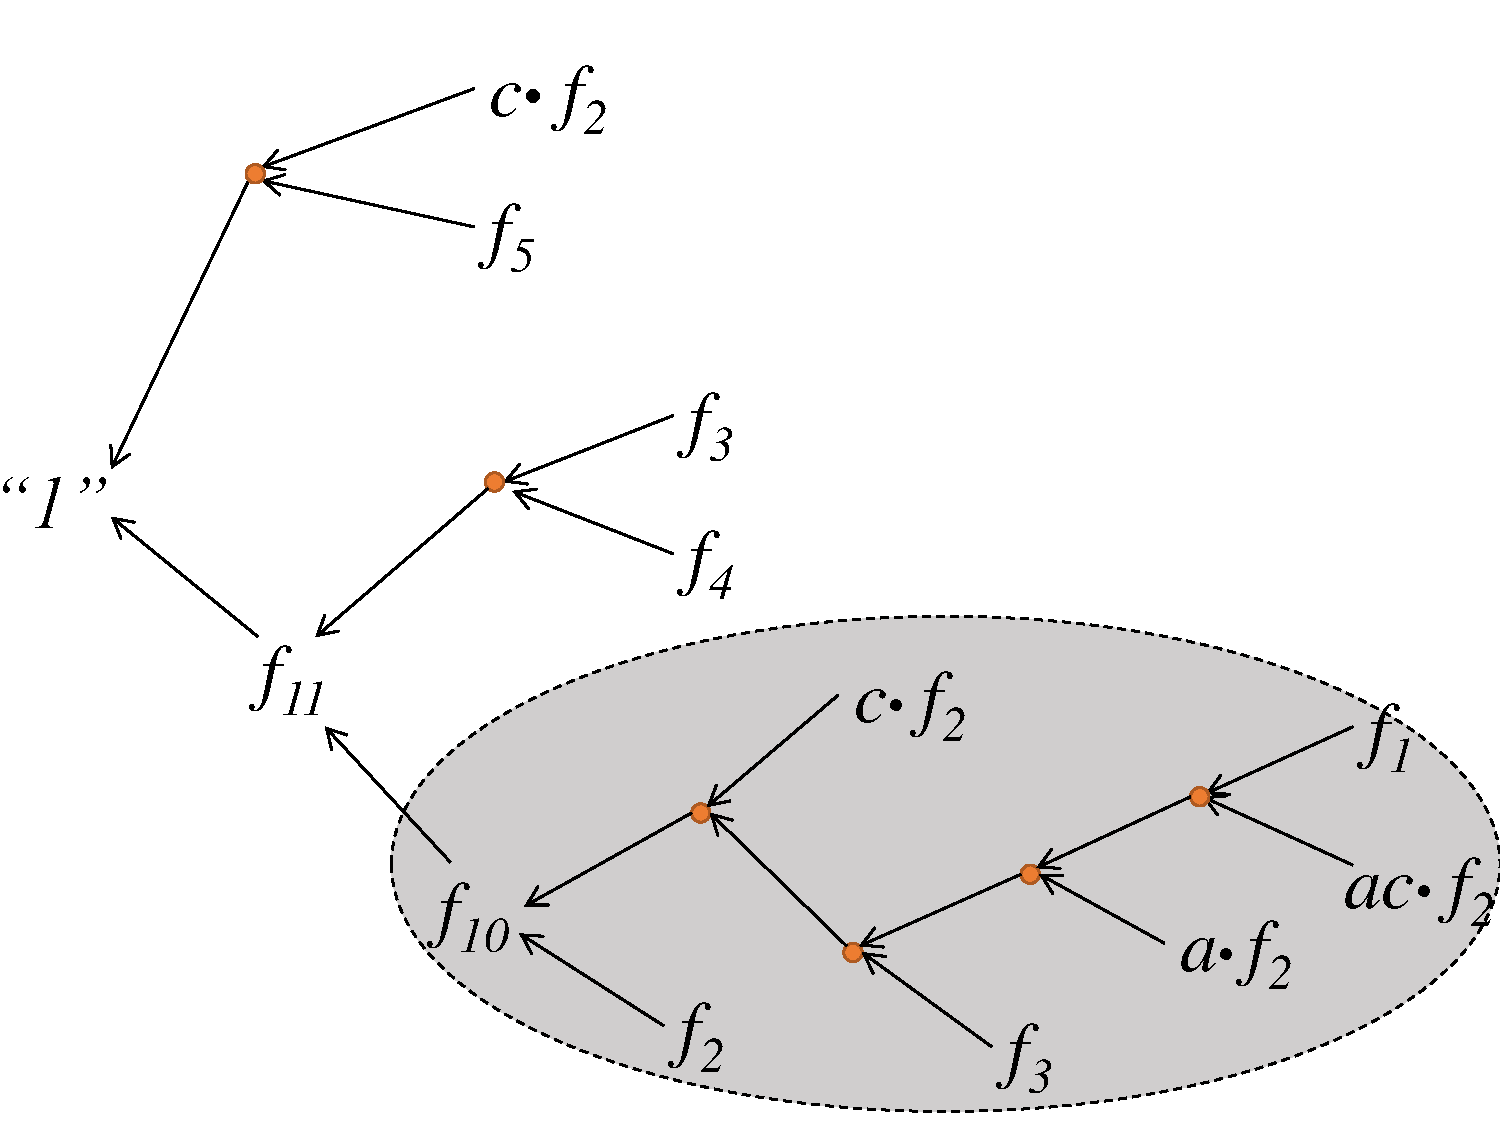
\includegraphics[width=3.5in]{./refutation_1.pdf}
\pause
\bi
\item $f_{10}=f_1-acf_2-af_2-f_3-cf_2-f_2 = f_1+acf_2+af_2+f_3+cf_2+f_2$
\item $1 = \F(f_1,f_2,f_3,f_4,f_5)\implies 1 \in \langle f_1,f_2,f_3,f_4,f_5\rangle \implies UNSAT$
\ei
\end{frame}
%%%%%%%%%%%%%%%%%%%%%%%%%%%%%%%%%%%%%%%%%%%%%%%%%%%%%%%%%%%%%
\begin{frame}{\large{Reducing size: redundancy in refutation tree}}
\bi
\item Expand: \begin{align*}
		1 &= \F(f_1,f_2,f_3,f_4,f_5)\\
		&= cf_2+f_5+\alert{f_{11}}\\
		&=cf_2+f_5+f_3+f_4+\alert{f_{10}}\\
		&=(cf_2 + f_5) + \dots + \mathbf{1\cdot f_3} + \dots + \mathbf{1\cdot
  f_3}+ \dots + (f_1 + acf_2)
		\end{align*}
\item UNSAT core reduced to $\{f_1,f_2,f_4,f_5\}$ which is {\bf minimal}
\item \alert{GB-core algorithm}:
	\bi
	\item Execute Buchberger's algorithm
	\item Recording data including Spoly, polynomials for division and remainder
	\item Terminate Buchberger's algorithm after recording remainder ``1"
	\item Build refutation tree and get UNSAT core
	\item Analyze recorded data, remove redundant polynomials from the core
	\ei
\ei
\end{frame}

%%%%%%%%%%%%%%%%%%%%%%%%%%%%%%%%%%%%%%%%%%%%%%%%%%%%%%%%%%%%%%%%%
\begin{frame}{\large{Reducing size: iterative refinement by reordering Spoly pairs}}
\bi
\item Spoly pair selection strategy: $(f_1,f_2)\to(f_1,f_3)\to(f_2,f_3)\to(f_1,f_4)\to(f_2,f_4)\to\cdots$  (Animation 3)
\item High likelihood in minimal core $\to$ Put ahead in Spoly queue $\to$ Faster approaching ``1" in GB-core $\to$ Smaller core
\ei
\vspace{-0.2in}
\begin{columns}[onlytextwidth]
\begin{column}{0.5\textwidth}
\begin{figure}
\centering
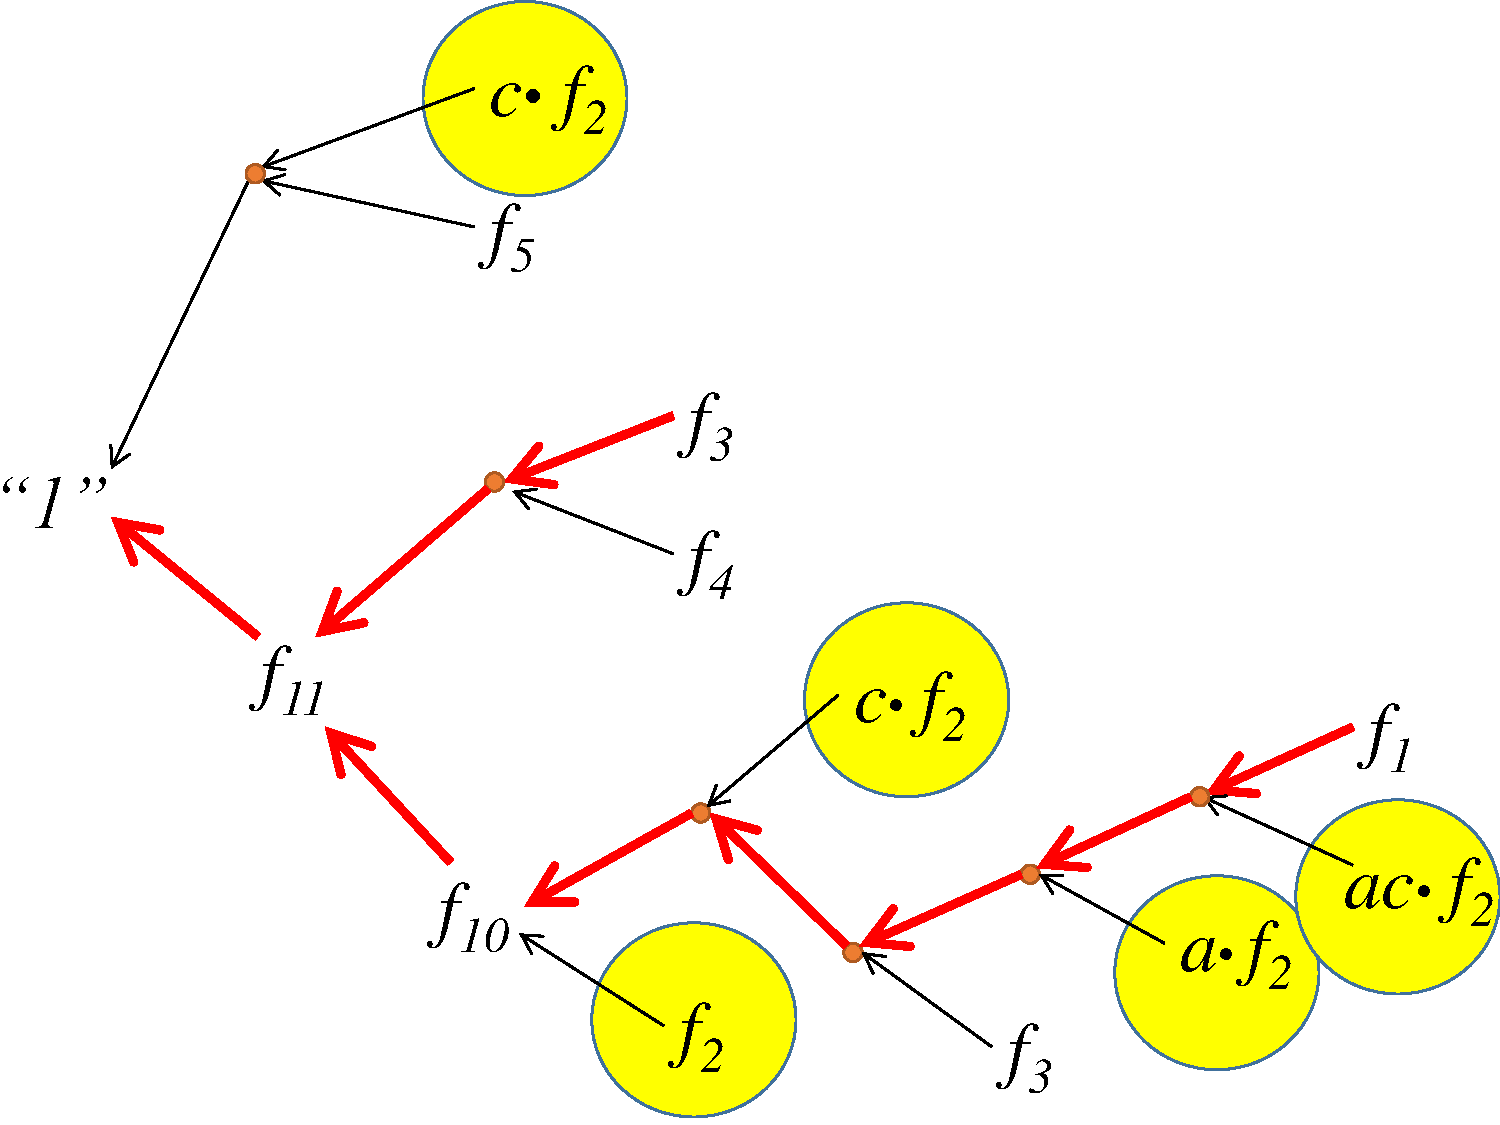
\includegraphics[scale=0.25]{refutation_2.pdf}
%\caption{Refutation distance \& frequency}
\end{figure}
\end{column}
\begin{column}{0.5\textwidth}
\bi
\item {\bf Refutation distance}: shortest path to leaf
\item Distance$\downarrow \to$ LT Degree$\downarrow \to$ Likelihood in minimal core $\uparrow$
\vspace{0.2in}
\item {\bf Frequency}: number of times $f_i$ appears in refutation tree
\ei
\end{column}
\end{columns}
\end{frame}

%%%%%%%%%%%%%%%%%%%%%%%%%%%%%%%%%%%%%%%%%%%%%%%%%%%%%%%%%%%%%%%%%%%
% use "alignat" to align to multiple columns

\begin{frame}{\large{Iterative refinement Example}}
\vspace{-0.1in}
\begin{alignat*}{4}
& f_1: x_1x_3+x_3 && ~~~f_2: x_2 + 1 && ~~~f_3: x_2x_3+x_2 \\
& f_4: x_2x_3 && ~~~f_5: x_2x_3 + x_2 + x_3 + 1 && ~~~f_6 : x_1x_2x_3 +x_1x_3
\end{alignat*}
\vspace{-0.5in}
\begin{columns}[onlytextwidth]
\begin{column}{0.6\textwidth}
\begin{figure}
\centering
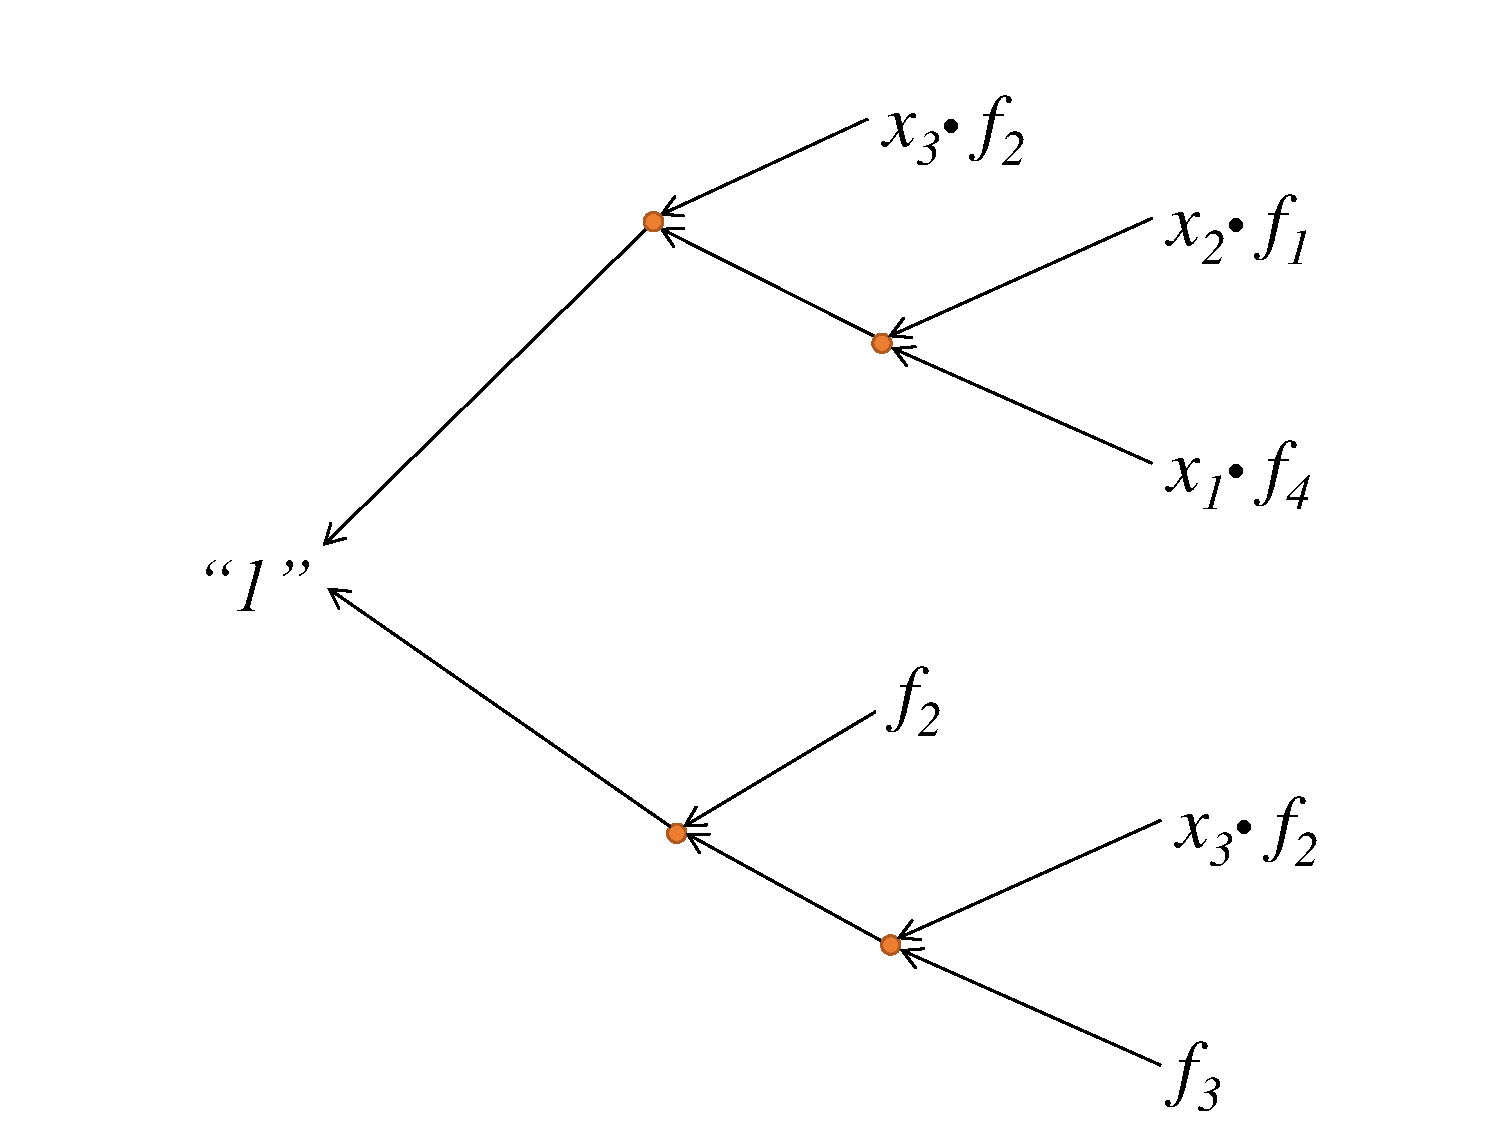
\includegraphics[scale=0.3]{iterative_1.pdf}
\end{figure}
\end{column}
\begin{column}{0.4\textwidth}
\bi
\item $F=\{f_1,f_2,\dots,f_6\}\in\mathbb{F}_2[x_1,x_2,x_3]$
\item UNSAT core: $f_1,f_2,f_3,f_4$
\item \alert{Refutation distance}: \\
		$f_2~~f_1~~f_3~~f_4$\\
		$2~~~3~~~3~~~3$
\item \alert{Frequency}:\\
		$f_1~~f_3~~f_4$\\
		$1~~~1~~~1$
\item Reorder: $\alert{f_2},f_1,f_3,f_4$
\ei
\end{column}
\end{columns}
\end{frame}

%%%%%%%%%%%%%%%%%%%%%%%%%%%%%%%%%%%%%%%%%%%%%%%%%%%%%%%%%%%%%%%%%%%
\begin{frame}{\large{Iterative refinement: iteration 2}}
\vspace{-0.1in}
\begin{alignat*}{4}
& f_1: x_1x_3+x_3 && ~~~f_2: x_2 + 1 && ~~~f_3: x_2x_3+x_2 \\
& f_4: x_2x_3 && ~~~f_5: x_2x_3 + x_2 + x_3 + 1 && ~~~f_6 : x_1x_2x_3 +x_1x_3
\end{alignat*}
\vspace{-0.5in}
\begin{columns}[onlytextwidth]
\begin{column}{0.6\textwidth}
\begin{figure}
\centering
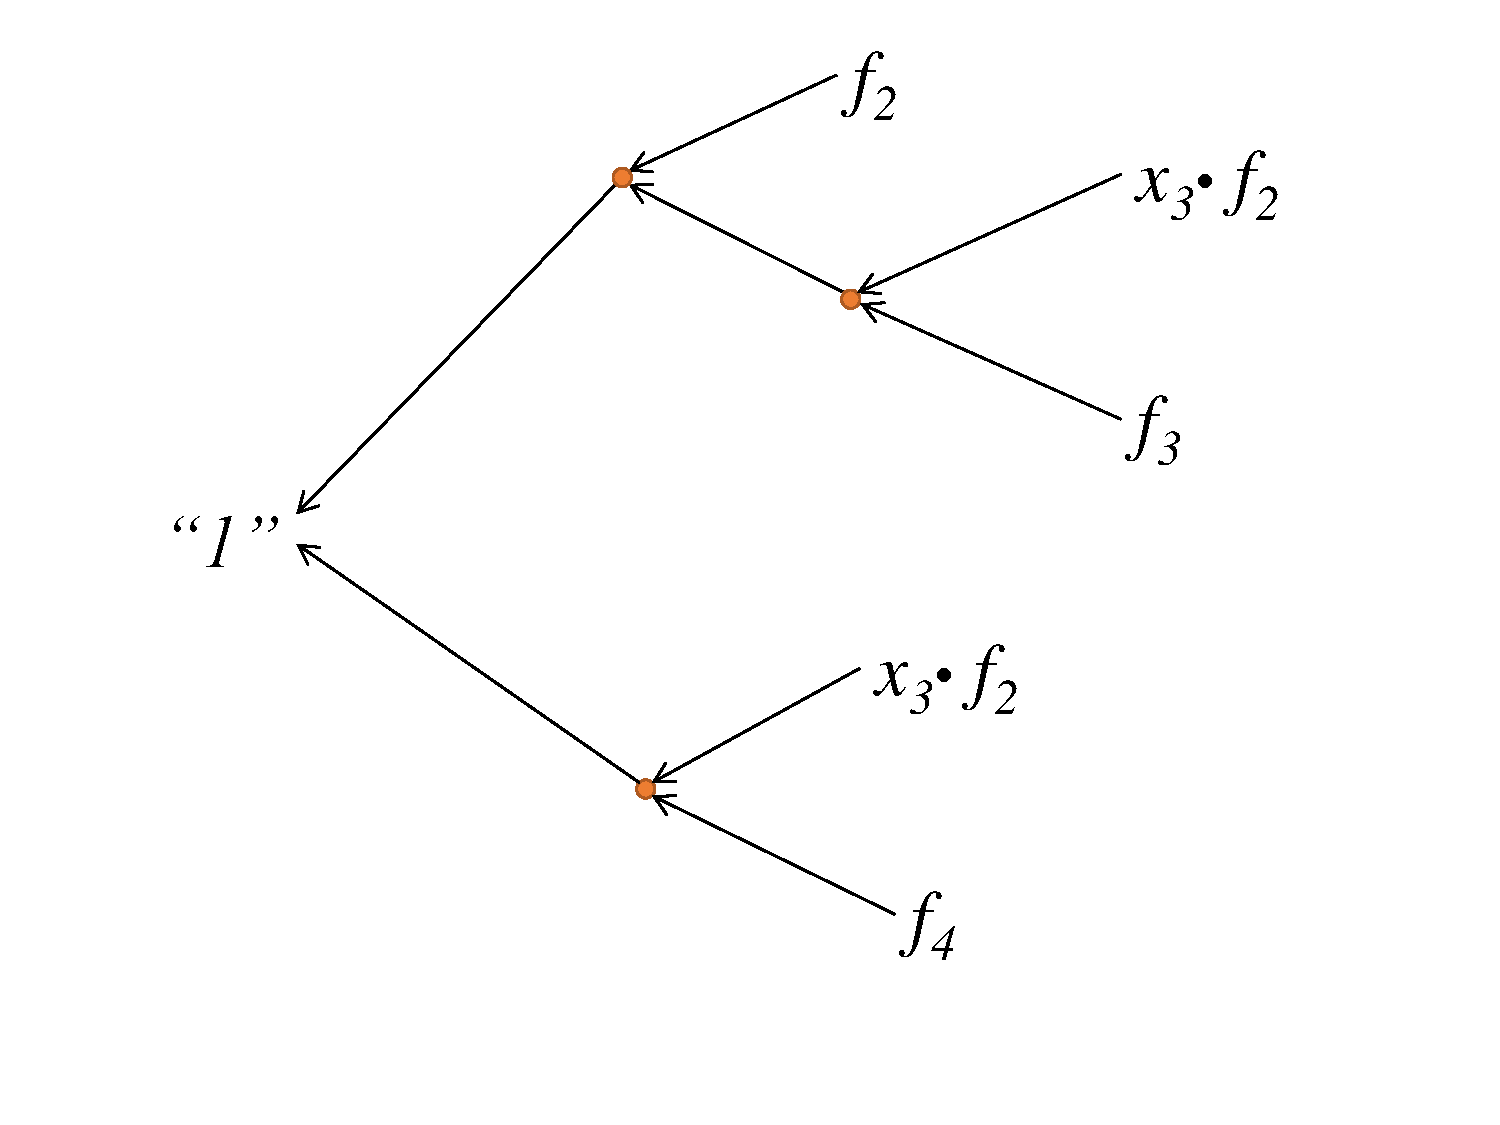
\includegraphics[scale=0.3]{iterative_2.pdf}
\end{figure}
\end{column}
\begin{column}{0.4\textwidth}
\bi
\item New order: $f_2,f_1,f_3,f_4$
\item Spoly pairs selection:\\
	$(\alert{f_2},f_1)\to(\alert{f_2},f_3)\to(f_1,f_3)\to(\alert{f_2},f_4)\to(f_1,f_4)\to(f_3,f_4)$
\item UNSAT core: $f_2,f_3,f_4$
\item \alert{Fixpoint reached}
\ei
\end{column}
\end{columns}
\end{frame}
%%%%%%%%%%%%%%%%%%%%%%%%%%%%%%%%%%%%%%%%%%%%%%%%%%%%%%%%%%%%%%%%%%%%

\begin{frame}{\large{Reducing size further using syzygy heuristic}}
\bi
\item Finding interdependencies: $f_i\in\langle F\setminus\{f_i\}\rangle$?
\item Given $F=\{f_1,\dots,f_s\}$, find $f_i = \sum_{j\neq i} h_jf_j$
\item Info lost in refutation tree/Buchberger's algorithm?
\item Inner loop of Buchberger's algorithm: \\
\hspace{0.2in}  $Spoly(f, g) \stackrel{G'}{\textstyle\longrightarrow}_+
r$ \\
\hspace{0.2in}  \alert{IF $r \neq 0$} THEN $G:= G \cup \{r\}$ \\
\hspace{0.2in}  \alert{IF $r = 0$} THEN Discard 

\item We collect division info when $r = 0$:
	\bi
	\item Record data for Spoly and polynomial division as in GB-core algorithm
	\ei
\item $Spoly(f_i,f_j)\xrightarrow{F}_+ 0\implies \alert{c_1f_1+c_2f_2+\cdots+c_sf_s = 0}$
\pause
\item $(c_1,c_2,\dots,c_s)$ is a {\bf syzygy} on $(f_1,f_2,\dots,f_s)$
\ei
\end{frame}

%%%%%%%%%%%%%%%%%%%%%%%%%%%%%%%%%%%%%%%%%%%%%%%%%%%%%%%%%%%%%%%%%%%%
\begin{frame}{\large{Reducing size further using syzygy heuristic}}
\bi
\item In a single syzygy, $c_i=1 \implies f_i = \sum_{j\neq i} h_jf_j$
\item In general cases, need to analyze all syzygies recorded
\item Collect $m$ syzygies as a system of polynomial equations, or a {\bf Syzygy Matrix}
\ei
\hspace{-0.1in}
\begin{minipage}{2.5in}
\begin{equation*} \label{eqn:syz}
 \begin{cases}
 c_1^1f_1+c_2^1f_2+\cdots+c_s^1f_s = 0\\
 c_1^2f_1+c_2^2f_2+\cdots+c_s^2f_s  = 0\\
 \ \ \ \ \ \  \vdots \\
 c_1^mf_1+c_2^mf_2+\cdots+c_s^mf_s = 0  
 \end{cases}
\end{equation*}
\end{minipage}
\hspace{-0.3in}
\begin{minipage}{2in}
%which can be represented in matrix form as:
\begin{center}
\begin{align*}
\label{mat:syzygy}
   \begin{bmatrix}
           c_1^1 & c_2^1 & \cdots & c_s^1 \\
           c_1^2 & c_2^2 & \cdots & c_s^2 \\
           \vdots & \vdots & \ddots & \vdots \\
           c_1^m & c_2^m & \cdots & c_s^m
         \end{bmatrix}
    \begin{bmatrix}
           f_{1} \\
           f_{2} \\
           \vdots \\
           f_{s}
         \end{bmatrix}
         &= 0
  \end{align*}

\end{center}
\end{minipage}
\end{frame}

%%%%%%%%%%%%%%%%%%%%%%%%%%%%%%%%%%%%%%%%%%%%%%%%%%%%%%%%%%%%%%%%%%%%%
\begin{frame}{\large{Reducing size: revisiting motivating example with syzygy}}
\vspace{-0.2in}
\begin{columns}[onlytextwidth]
\begin{column}{0.5\textwidth}
\begin{figure}
\centering
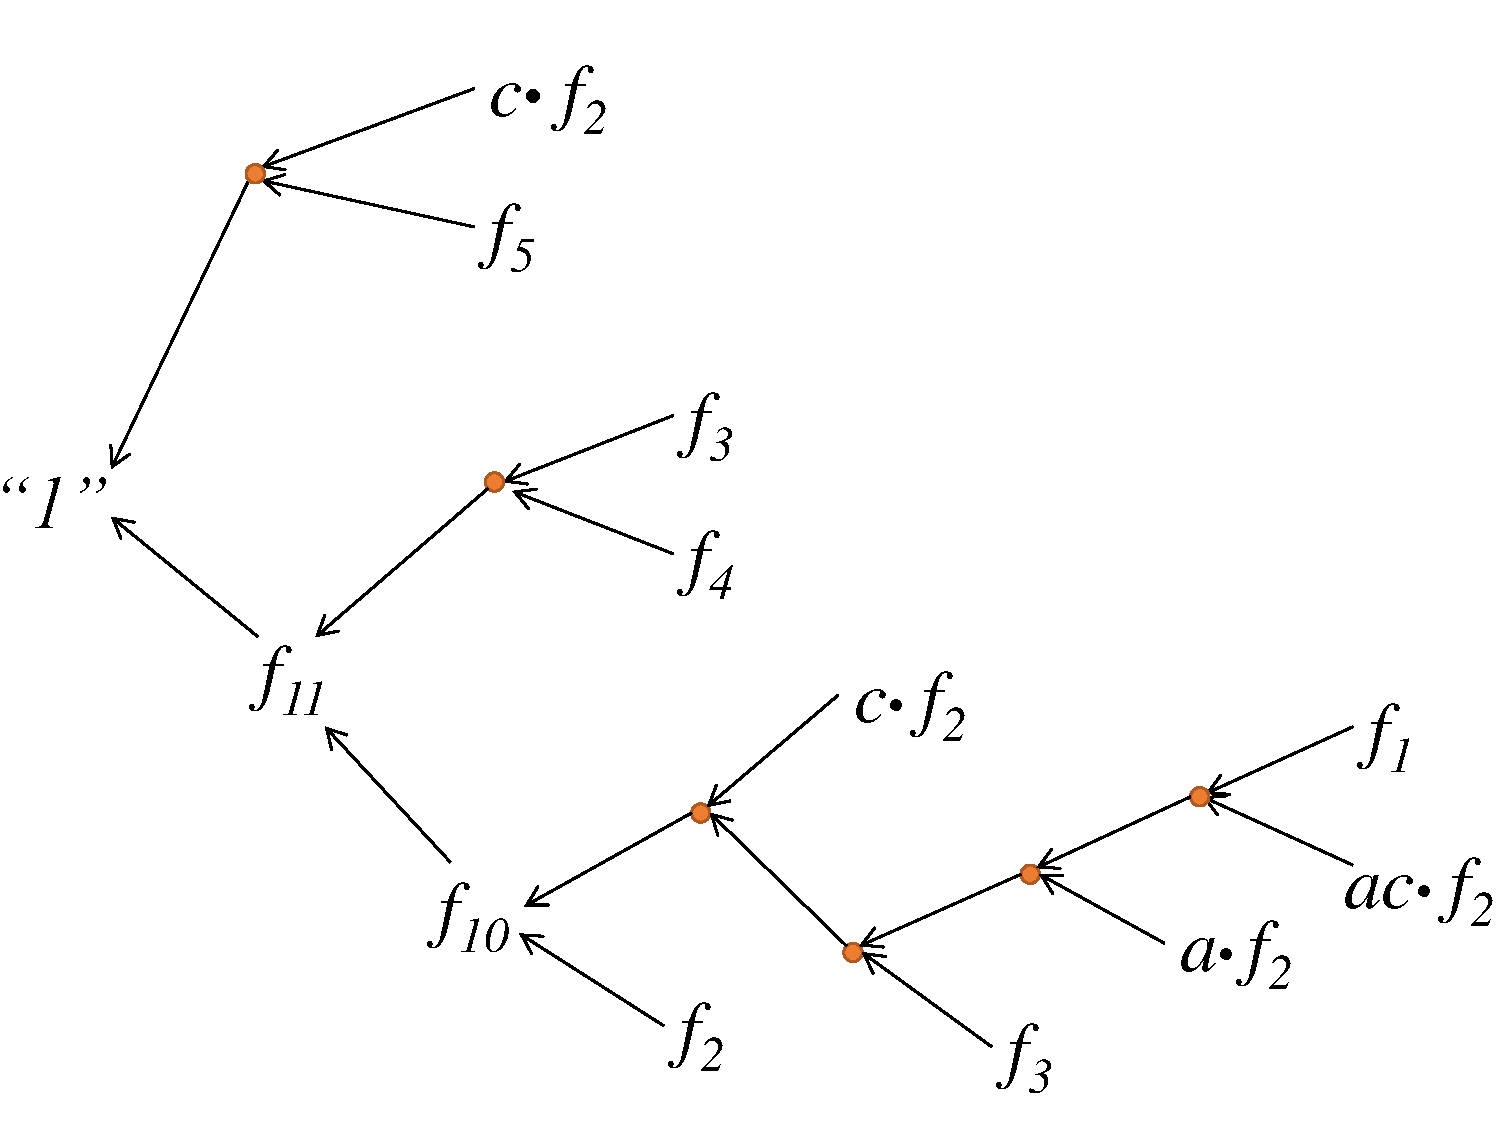
\includegraphics[scale=0.25]{refutation_tree.pdf}
\end{figure}
\end{column}
\begin{column}{0.5\textwidth}
\bi
\item Recorded in Buchberger's Algo:\\
$Spoly(f_1,f_2)\xrightarrow{F}_+ f_{10}$\\
$Spoly(f_3,f_4)\xrightarrow{F}_+ f_{11}$\\
$Spoly(f_2,f_5)\xrightarrow{F}_+ 1$
\item Discarded in Buchberger's Algo:\\
$Spoly(f_1,f_3)\xrightarrow{F}_+ 0$\\
$Spoly(f_2,f_3)\xrightarrow{F}_+ 0$\\
$\dots$\\
$Spoly(f_1,f_5)\xrightarrow{F}_+ 0$
\ei
\end{column}
\end{columns}
\end{frame}

%%%%%%%%%%%%%%%%%%%%%%%%%%%%%%%%%%%%%%%%%%%%%%%%%%%%%%%%%%%%%%%%
\begin{frame}{\large{Syzygy example: setup}}
\bi
\item Syzygy matrix:
\ei
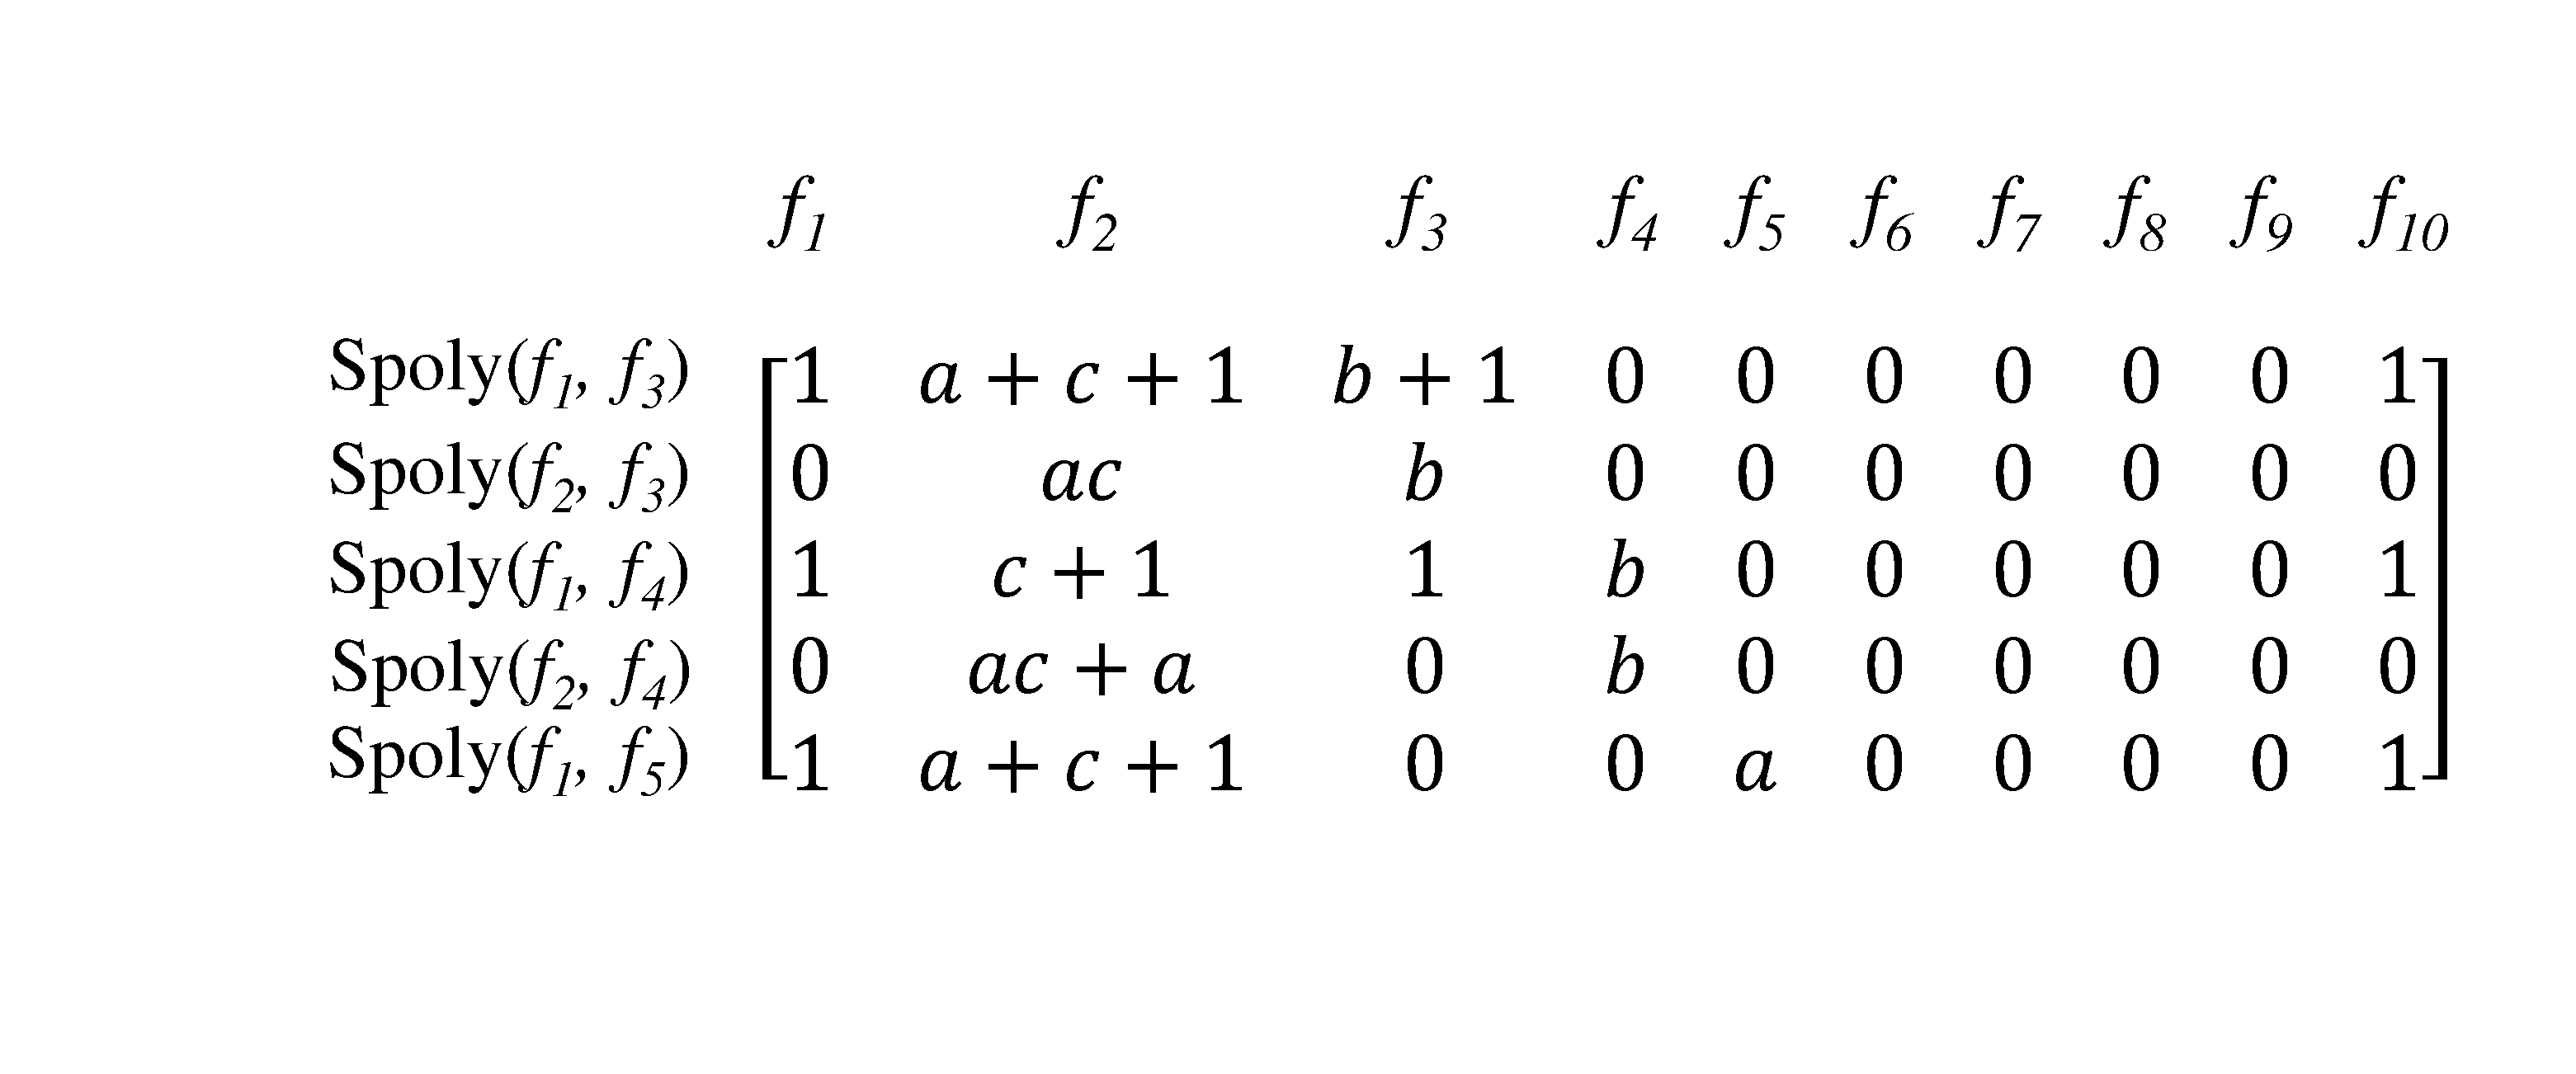
\includegraphics[width=4.5in]{./syzygy_1.pdf}
\pause
\llap{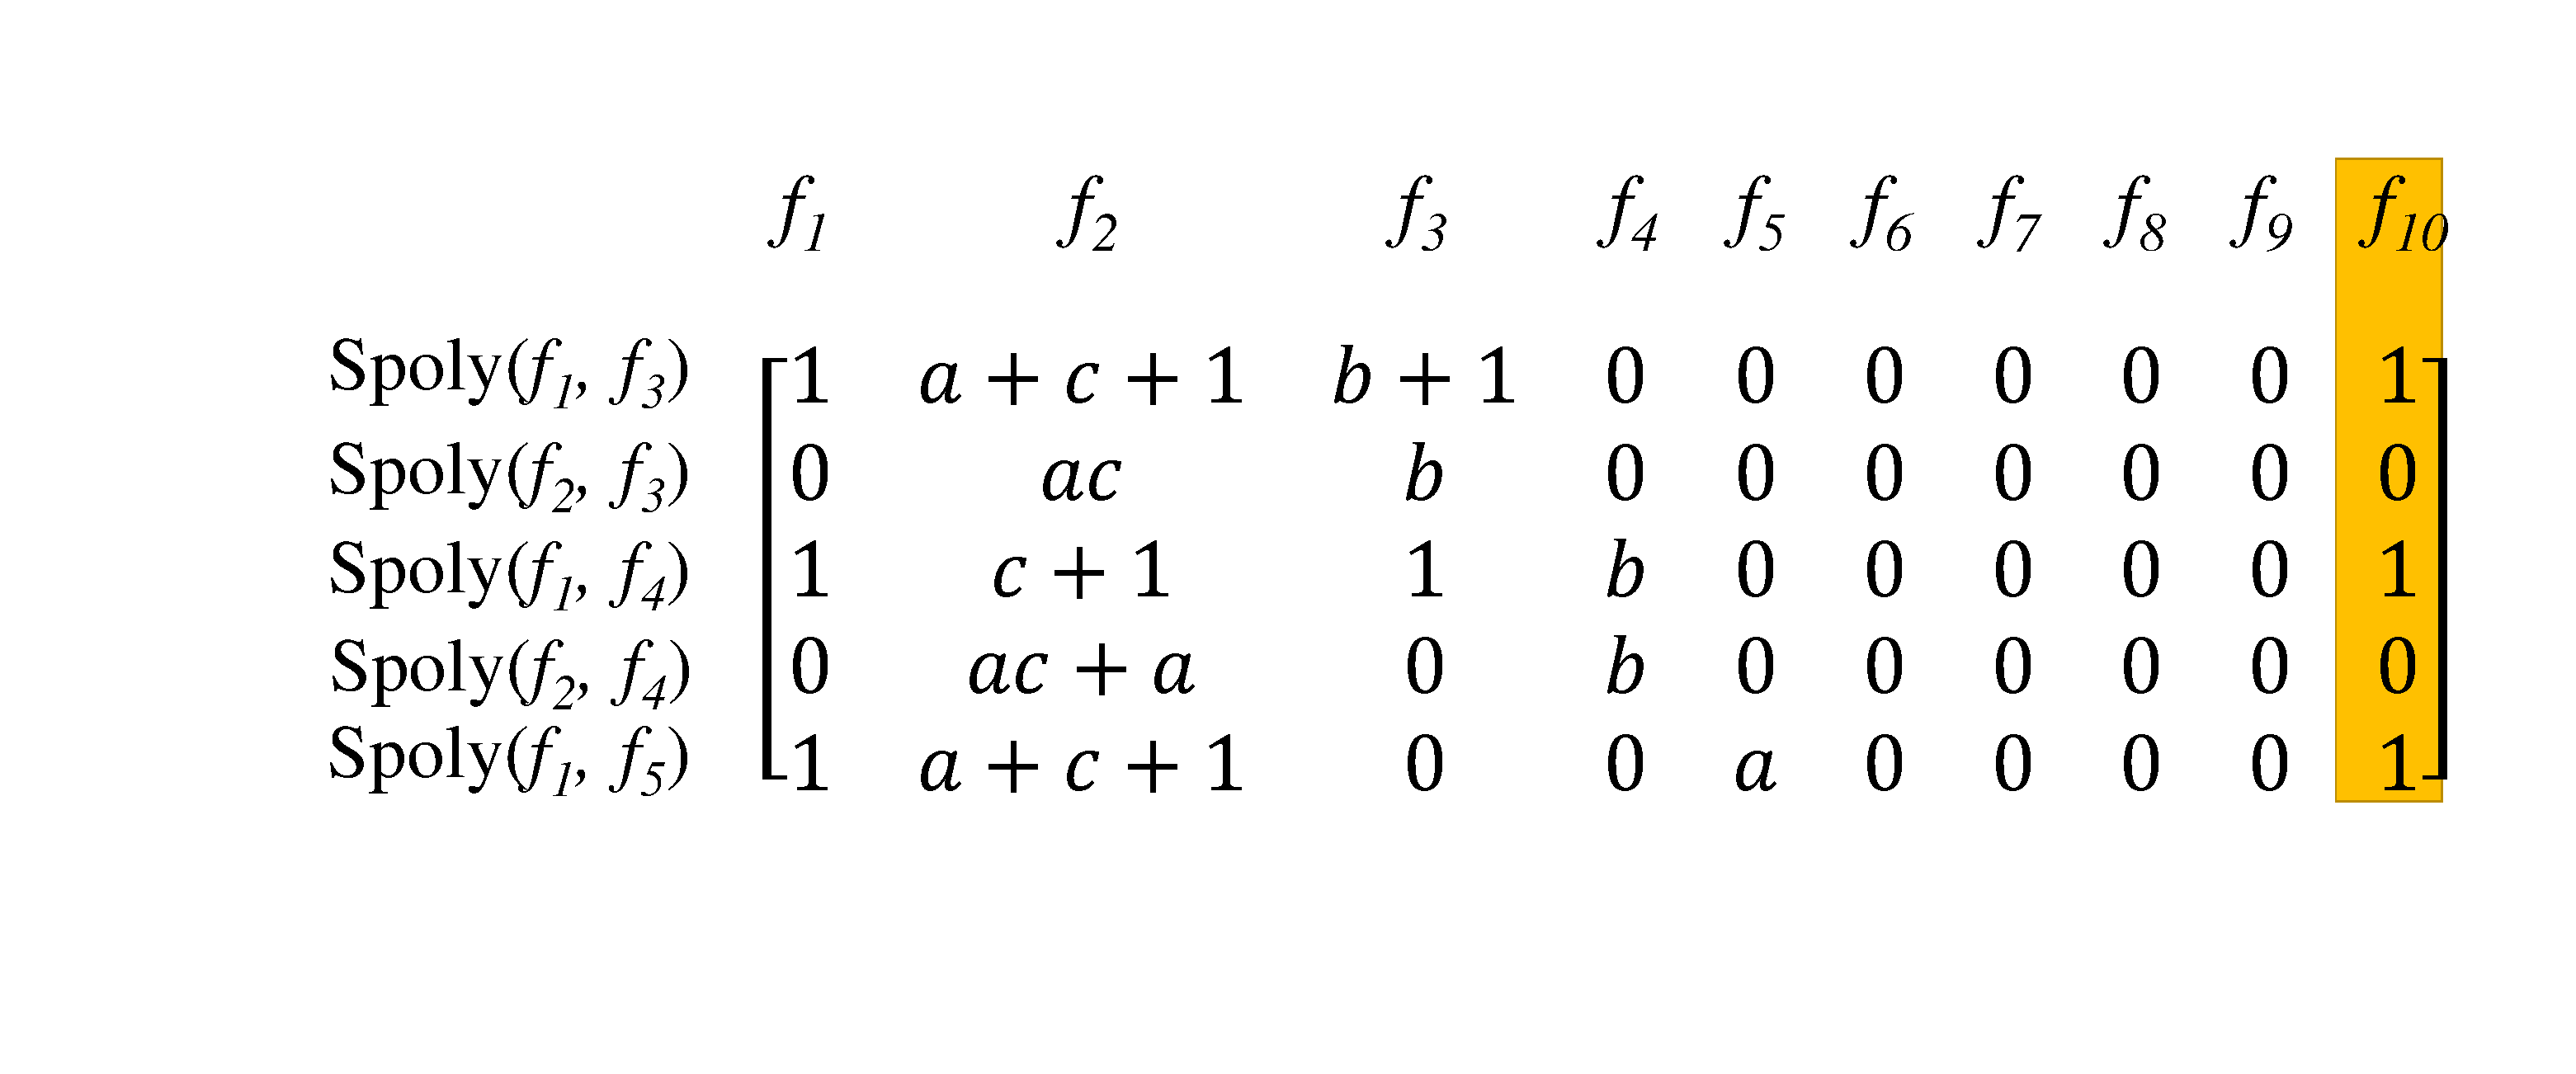
\includegraphics[width=4.5in]{./syzygy_2.pdf}}
\bi
\item rows: syzygies
\item $J = \langle f_1,f_2,\dots,f_9\rangle$
\item $f_{10}\in J$
\ei
\end{frame}
%%%%%%%%%%%%%%%%%%%%%%%%%%%%%%%%%%%%%%%%%%%%%%%%%%%%%%%%%%%%%%%
\begin{frame}{\large{Syzygy Example: refine syzygy matrix}}
\bi
\item Considering $f_{10}=f_1-acf_2-af_2-f_3-cf_2-f_2 = f_1+acf_2+af_2+f_3+cf_2+f_2$
\ei
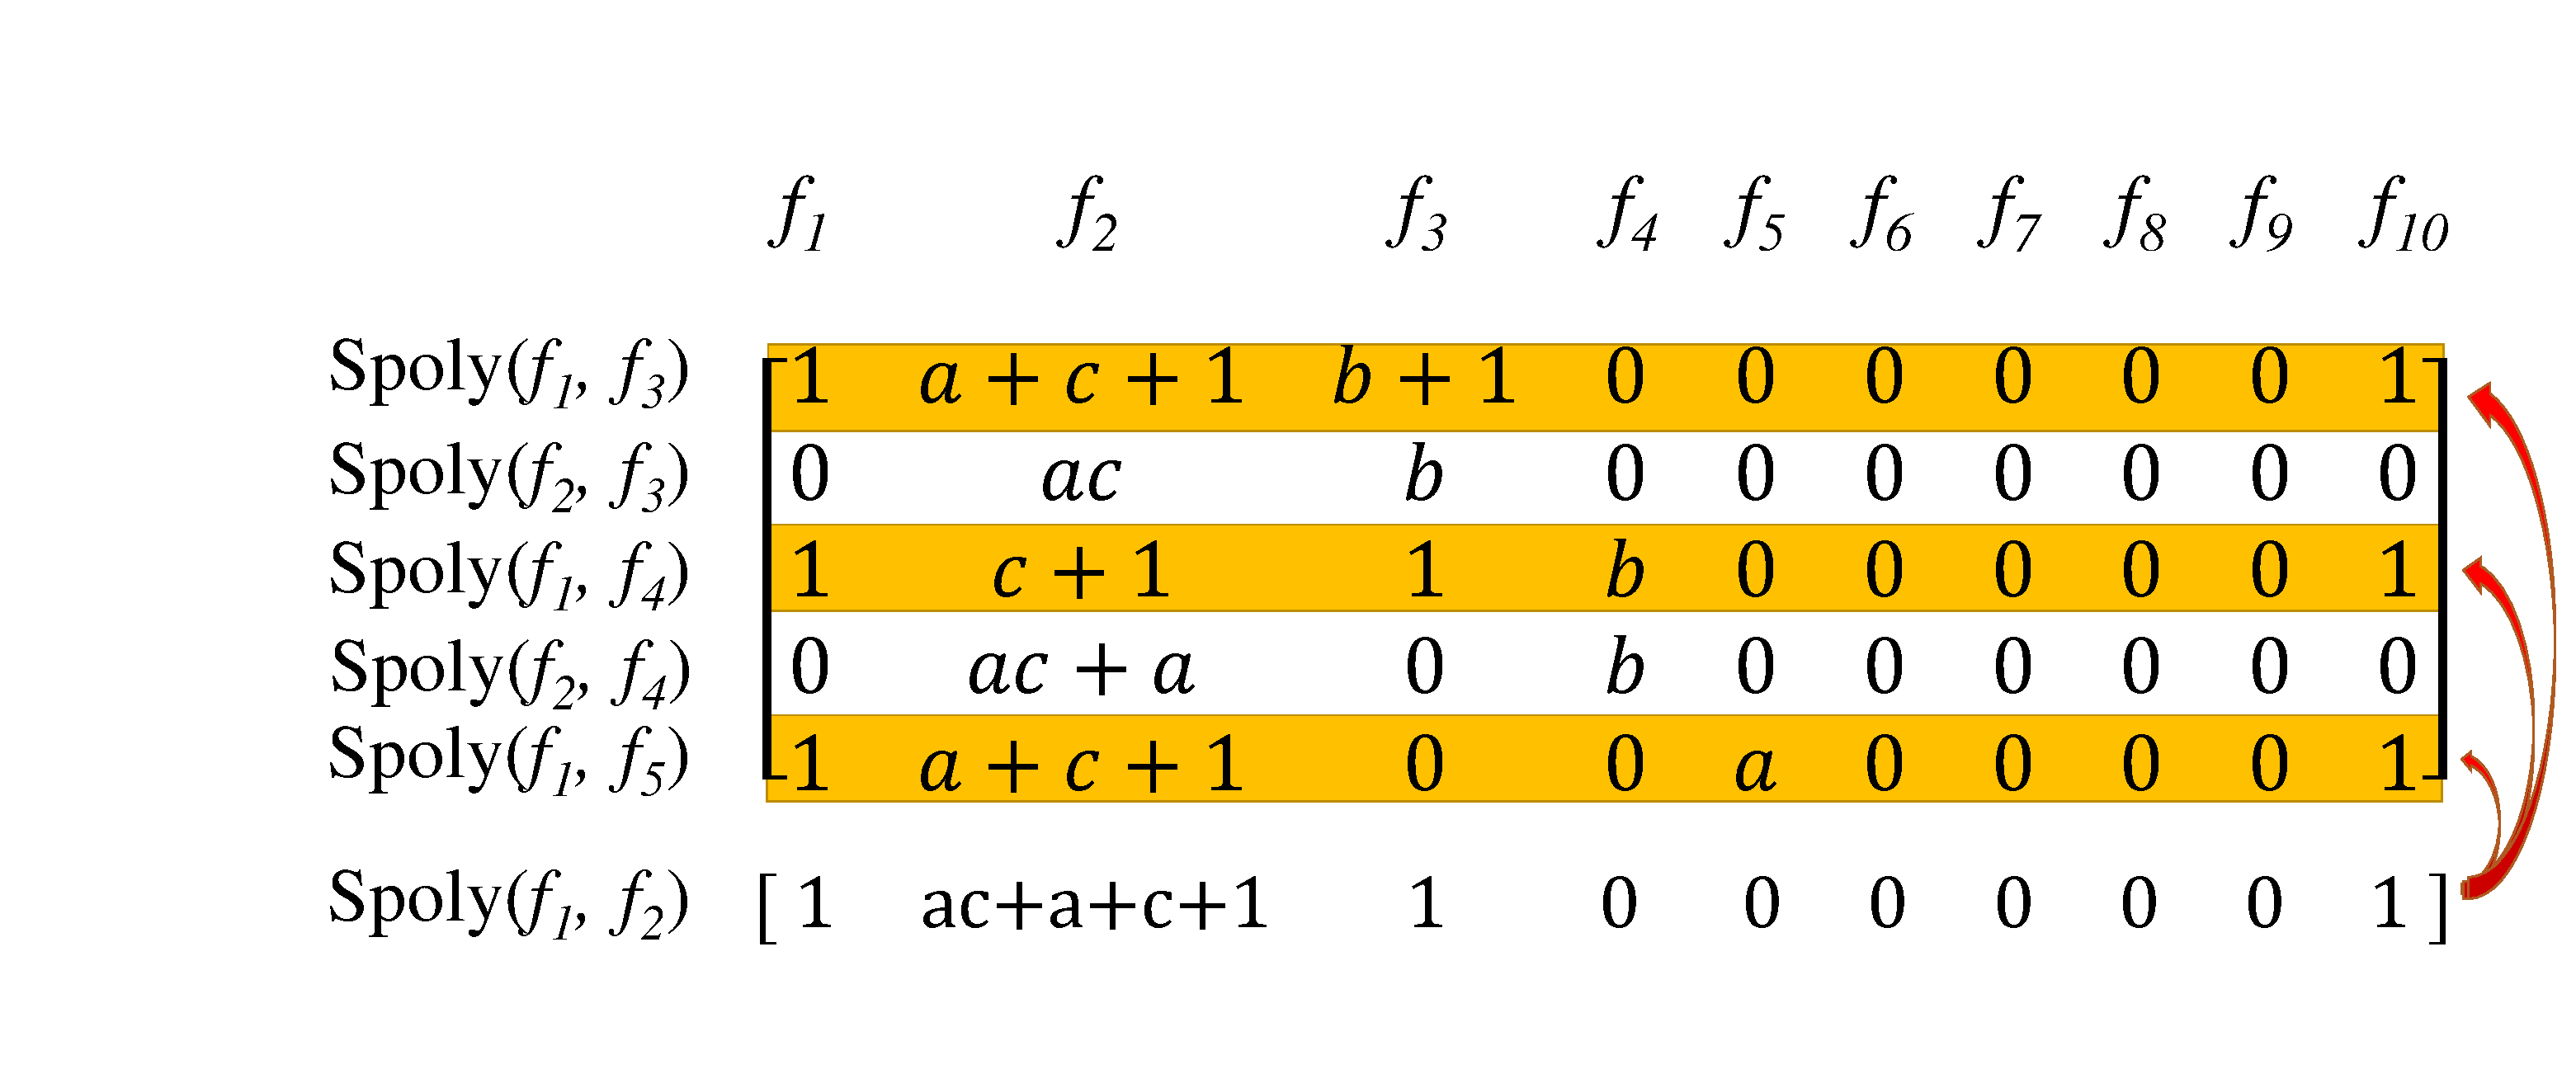
\includegraphics[width=4.5in]{./syzygy_3.pdf}
\end{frame}
%%%%%%%%%%%%%%%%%%%%%%%%%%%%%%%%%%%%%%%%%%%%%%%%%%%%%%%%%%%%%%
\begin{frame}{\large{Syzygy example: derive interdependency}}
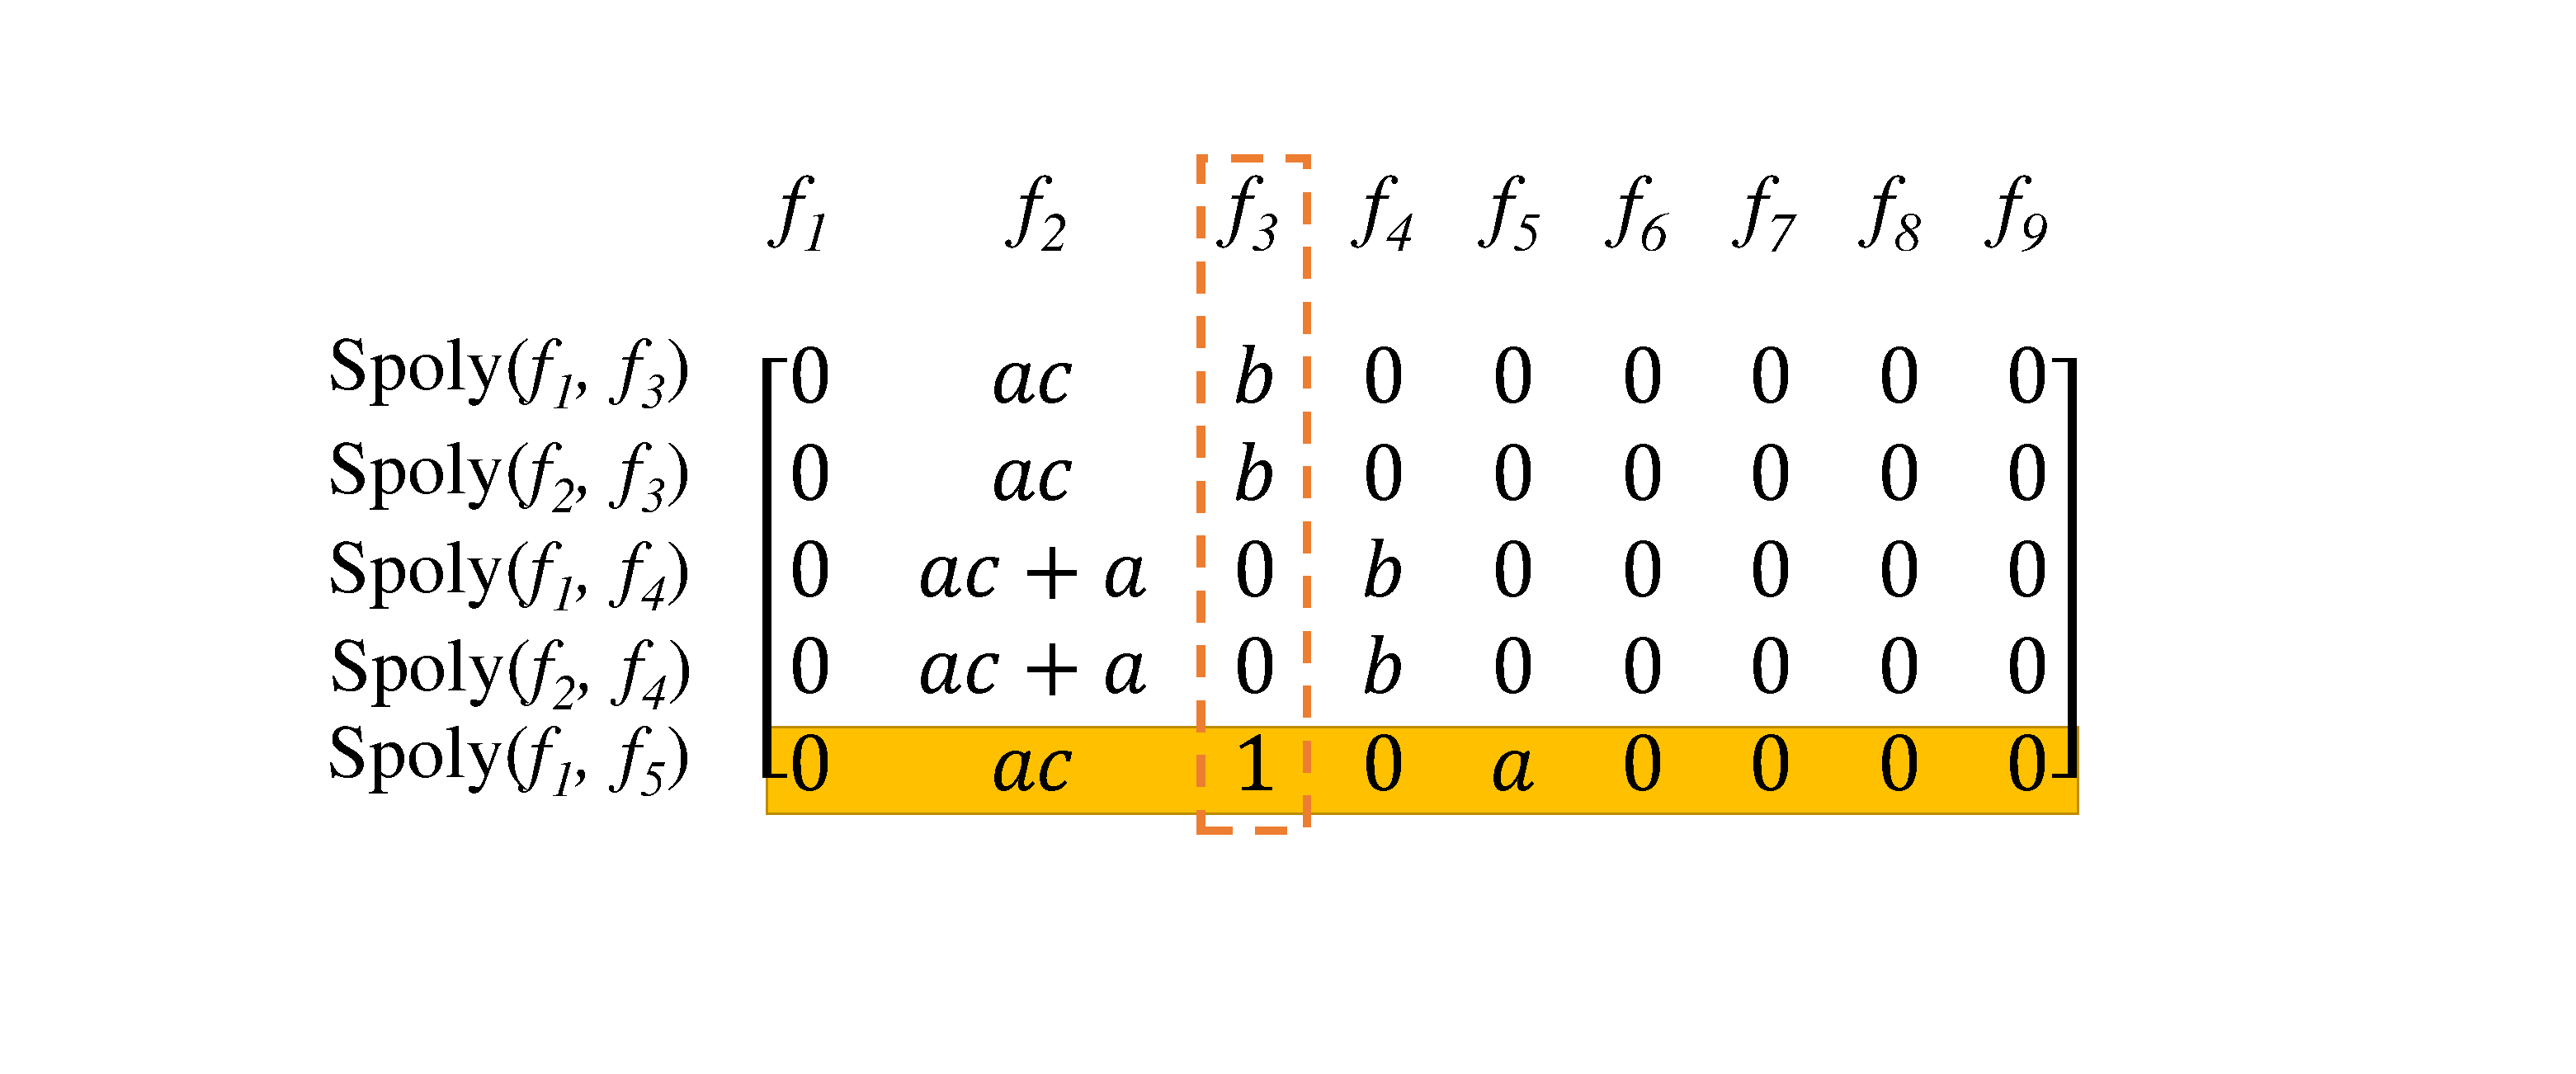
\includegraphics[width=4.5in]{./syzygy_4.pdf}
\bi
\item Column $f_3$ contains ``1", means:\\
$1\cdot f_3 + ac f_2 + a f_5 = 0\Leftrightarrow f_3 = acf_2+af_5$
\item Generalization of this strategy refer to the paper
\ei
\end{frame}
%%%%%%%%%%%%%%%%%%%%%%%%%%%%%%%%%%%%%%%%%%%%%%%%%%%%%%%%%%%%%%%
\begin{frame}{\large{Overall Approach}}
\begin{algorithm}[H] % note [hbt] will fail in beamer
\SetAlgoNoLine
 \KwIn{A set of UNSAT polynomials $F$} 
 \KwOut{A subset $F'\subset F$ remains UNSAT}
 $G \gets F$\;
  \Repeat{$G=F'$}
  {
	$F' = G$\;
  	$G \gets $GB-core($F'$ with order $>$)\;
	Update order $>$\;
  }
  $F'\gets$syzygy\_heuristic($G$)\;
\Return{$F'$}
\caption {UNSAT core extraction based on Gr\"obner basis algorithm}
\end{algorithm}
\end{frame}

%%%%%%%%%%%%%%%%%%%%%%%%%%%%%%%%%%%%%%%%%%%%%%%%%%%%%%%%%%%%%%
\begin{frame}{\large{Experiment results: UNSAT core extraction}}
\centering{Table of selected benchmarks}\\
\centering{I:single GB-core; II: Iterative GB-core; III: syzygy}
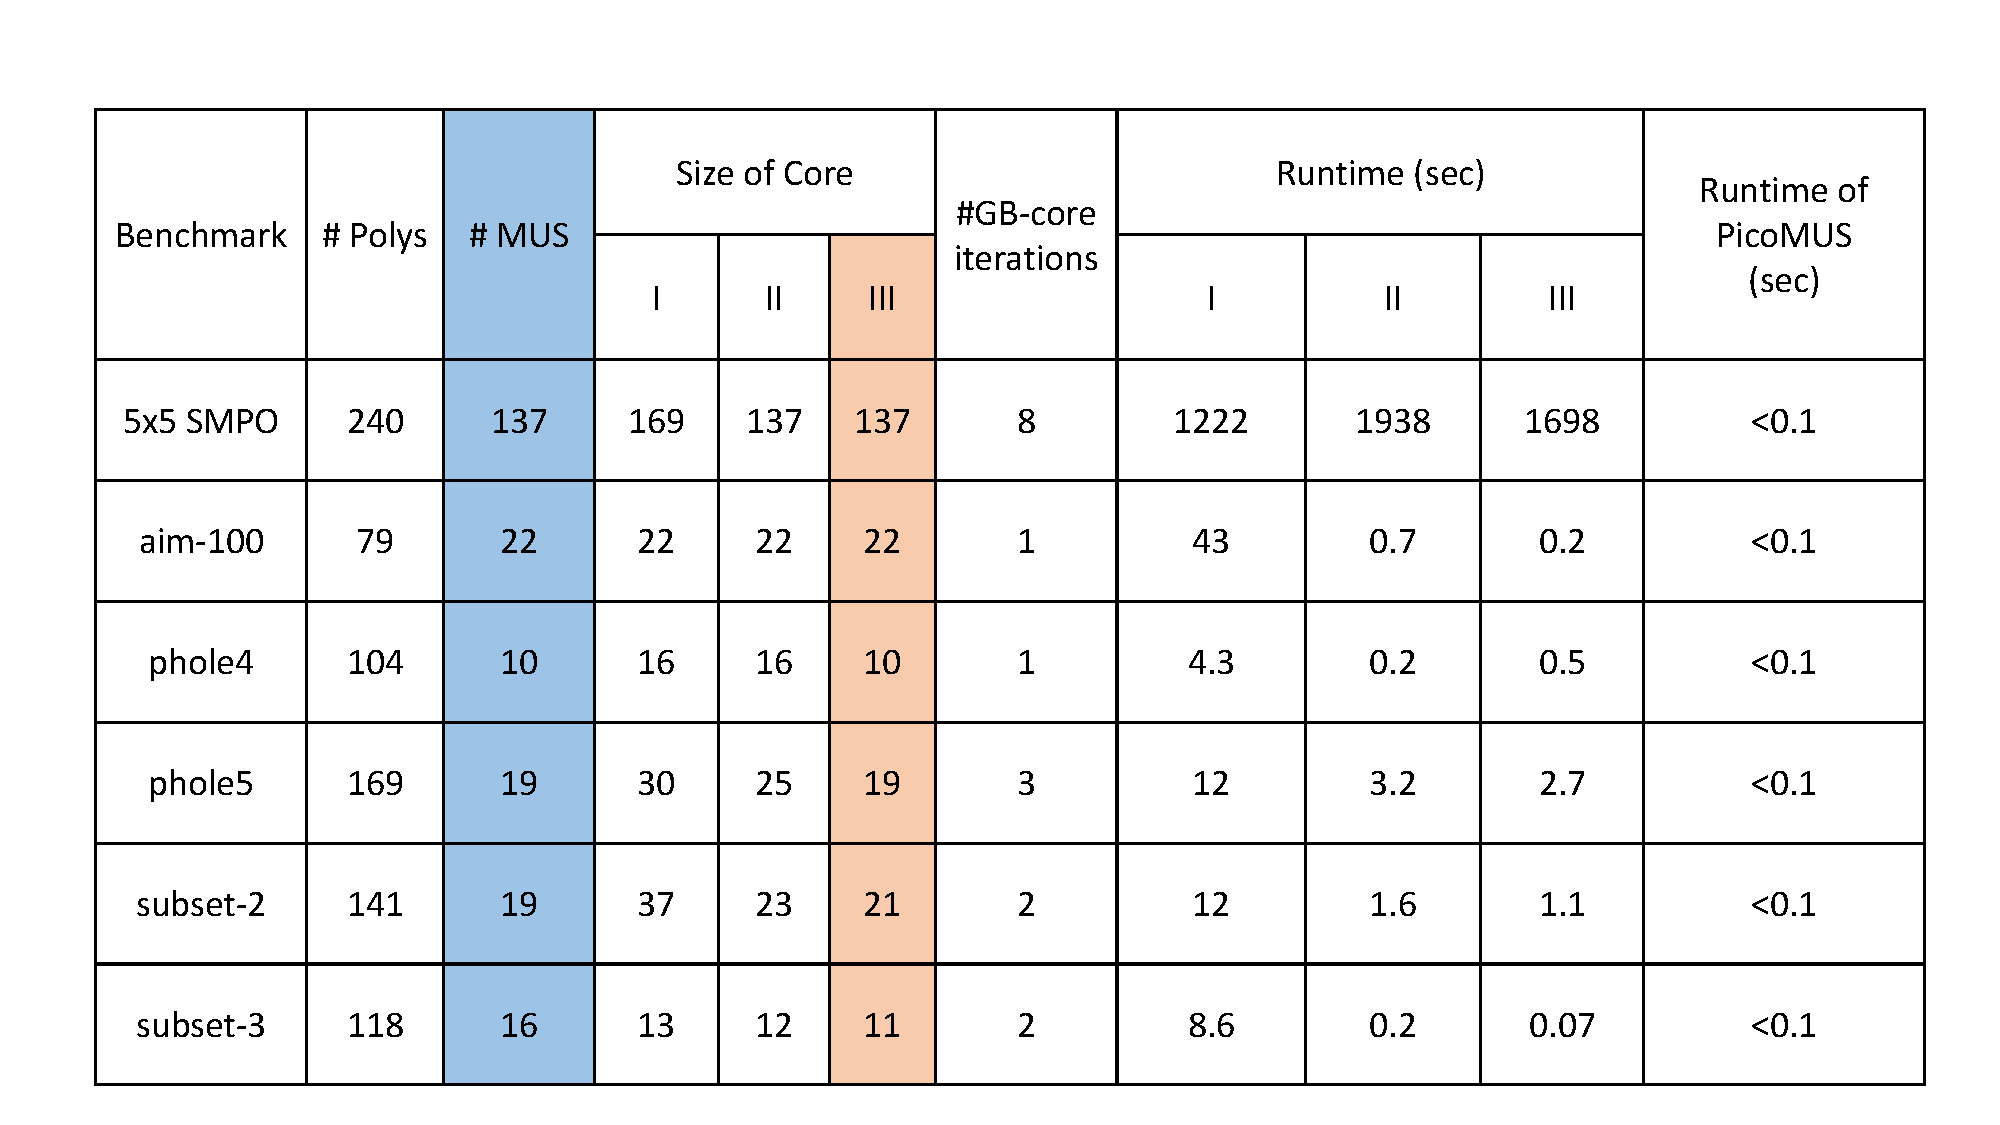
\includegraphics[width=4.5in]{./table_cp2016.pdf}

\end{frame}
%%%%%%%%%%%%%%%%%%%%%%%%%%%%%%%%%%%%%%%%%%%%%%%%%%%%%%%%%%%%%%
\begin{frame}{\large{Application to abstraction refinement}}
\vspace{-0.1in}
\begin{figure}
\centering
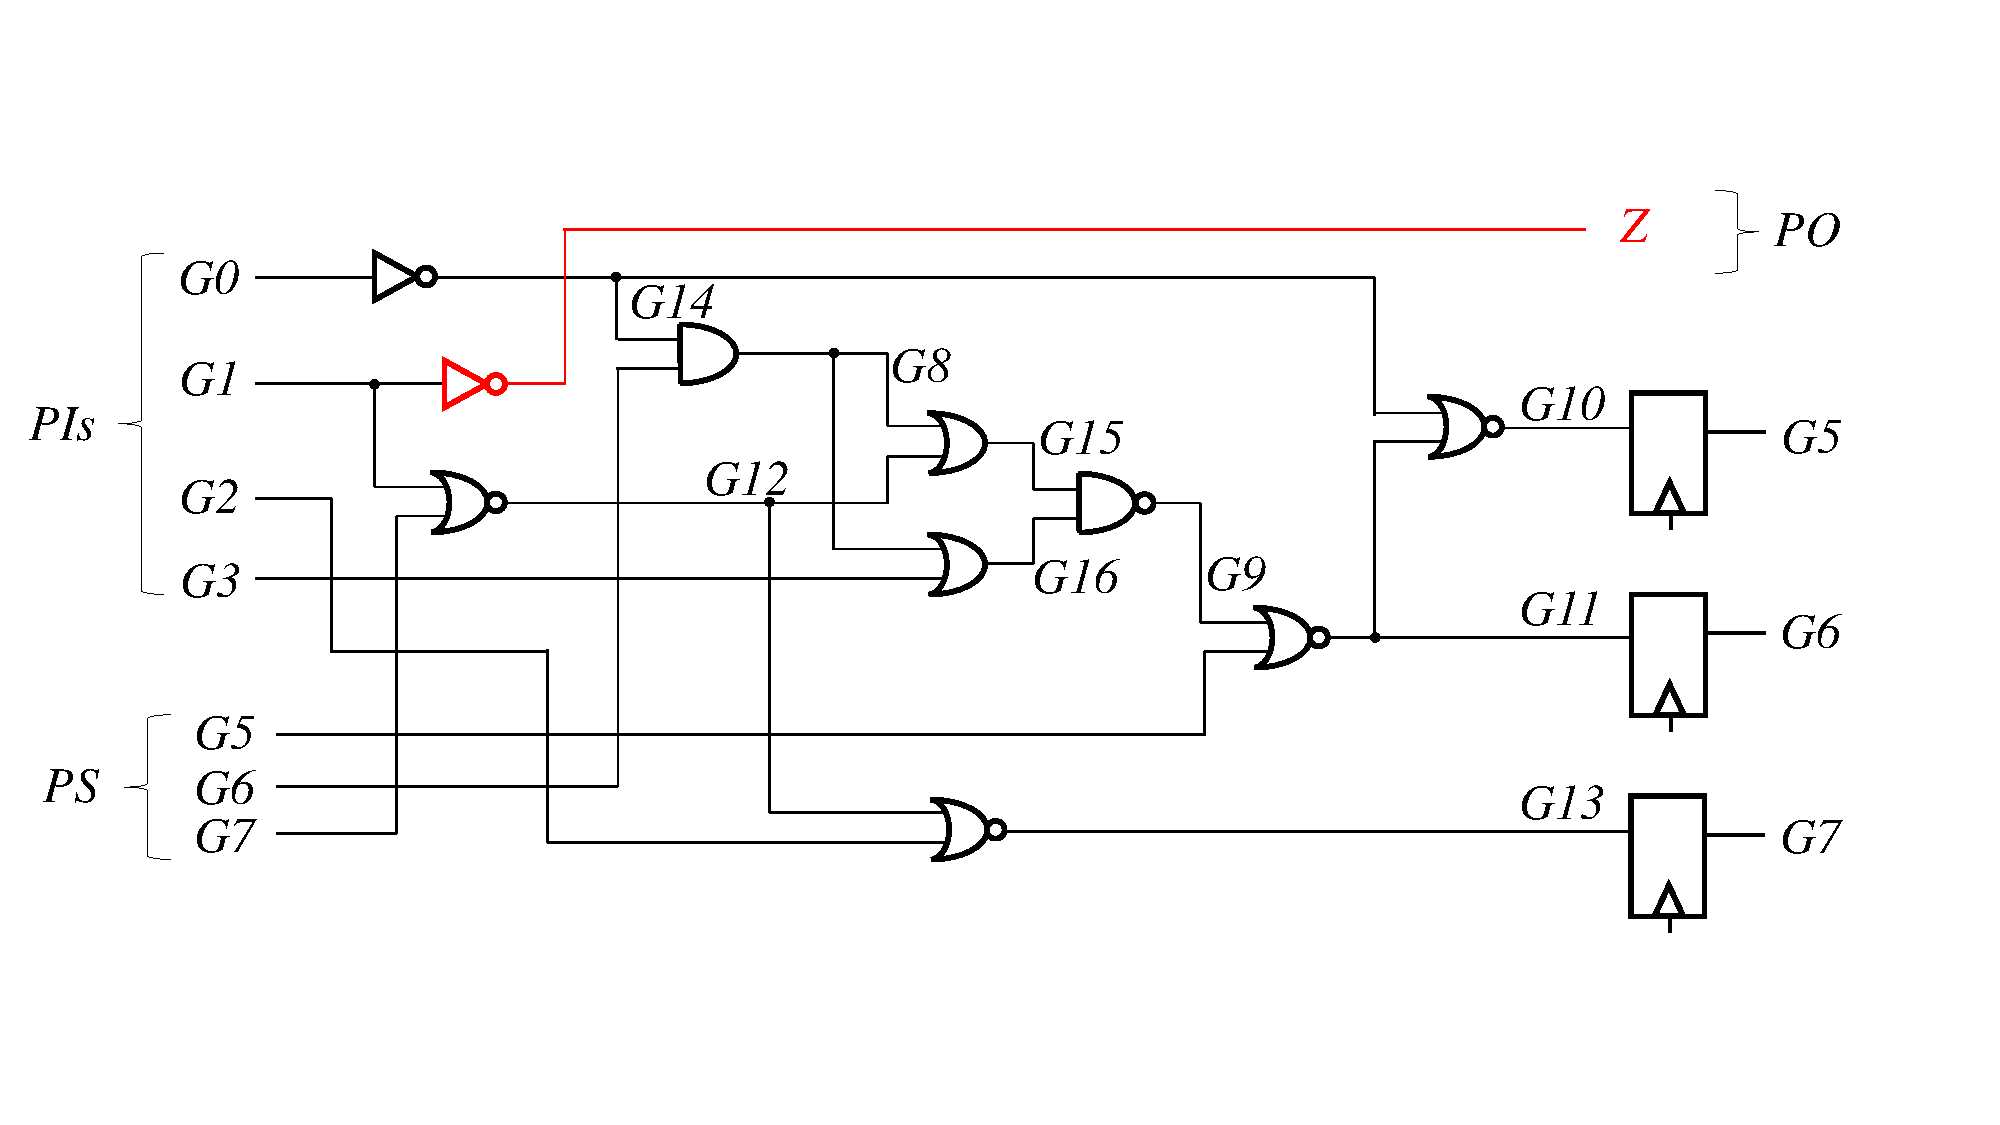
\includegraphics[scale=0.35]{../newfig/s27.pdf}
\end{figure}
\vspace{-0.3in}
\bi
\item PS = $\{G7,G6,G5\}$, NS = $\{G13,G11,G10\}$: 8 states
\item Property $p = {\bf AG}( (\neg G13) {\bf U} (\neg Z) )$
\item $k$-BMC without abstraction refinement: when $k=3$ prove $PASS$
\ei
\end{frame}
%%%%%%%%%%%%%%%%%%%%%%%%%%%%%%%%%%%%%%%%%%%%%%%%%%%%%%%%%%%%%%
\begin{frame}{\large{Application to abstraction refinement}}
\bi
\item Circuit ideal when $k=0$:
\ei
\begin{align*}
I = \langle & G14+1+G0, G8+G14\cdot G6, G15+G12+G8+G12\cdot G8,\\ 
	& G16+G3+G8+G3\cdot G8, G9+1+G16\cdot G15, \\ 
	& G10+1+G14+G11+G14\cdot G11, G11+1+G5+G9+G5\cdot G9, \\
	& G12+1+G1+G7+G1\cdot G7, G13+1+G2+G12+G2\cdot G12, \\
	& Z+1+G1, \\
	& \text{(Initial state 000 )} G5, G6, G7 \rangle;
\end{align*}
\vspace{-0.2in}
\bi
\item Property: $\neg p = Z\cdot G13 + 1$
\item UNSAT core: \begin{align*}
Core(I\land \neg p) =& G12+1+G1+\alert{G7}+G1\cdot \alert{G7},\\
&\alert{G13}+1+G2+G12+G2\cdot G12, \\
& Z+1+G1, \alert{G7};
\end{align*}
\ei
\end{frame}
%%%%%%%%%%%%%%%%%%%%%%%%%%%%%%%%%%%%%%%%%%%%%%%%%%%%%%%%%%%%%%
\begin{frame}{\large{Application to abstraction refinement}}
\vspace{-0.1in}
\begin{columns}[onlytextwidth]
\begin{column}{0.5\textwidth}
\begin{figure}
\centering
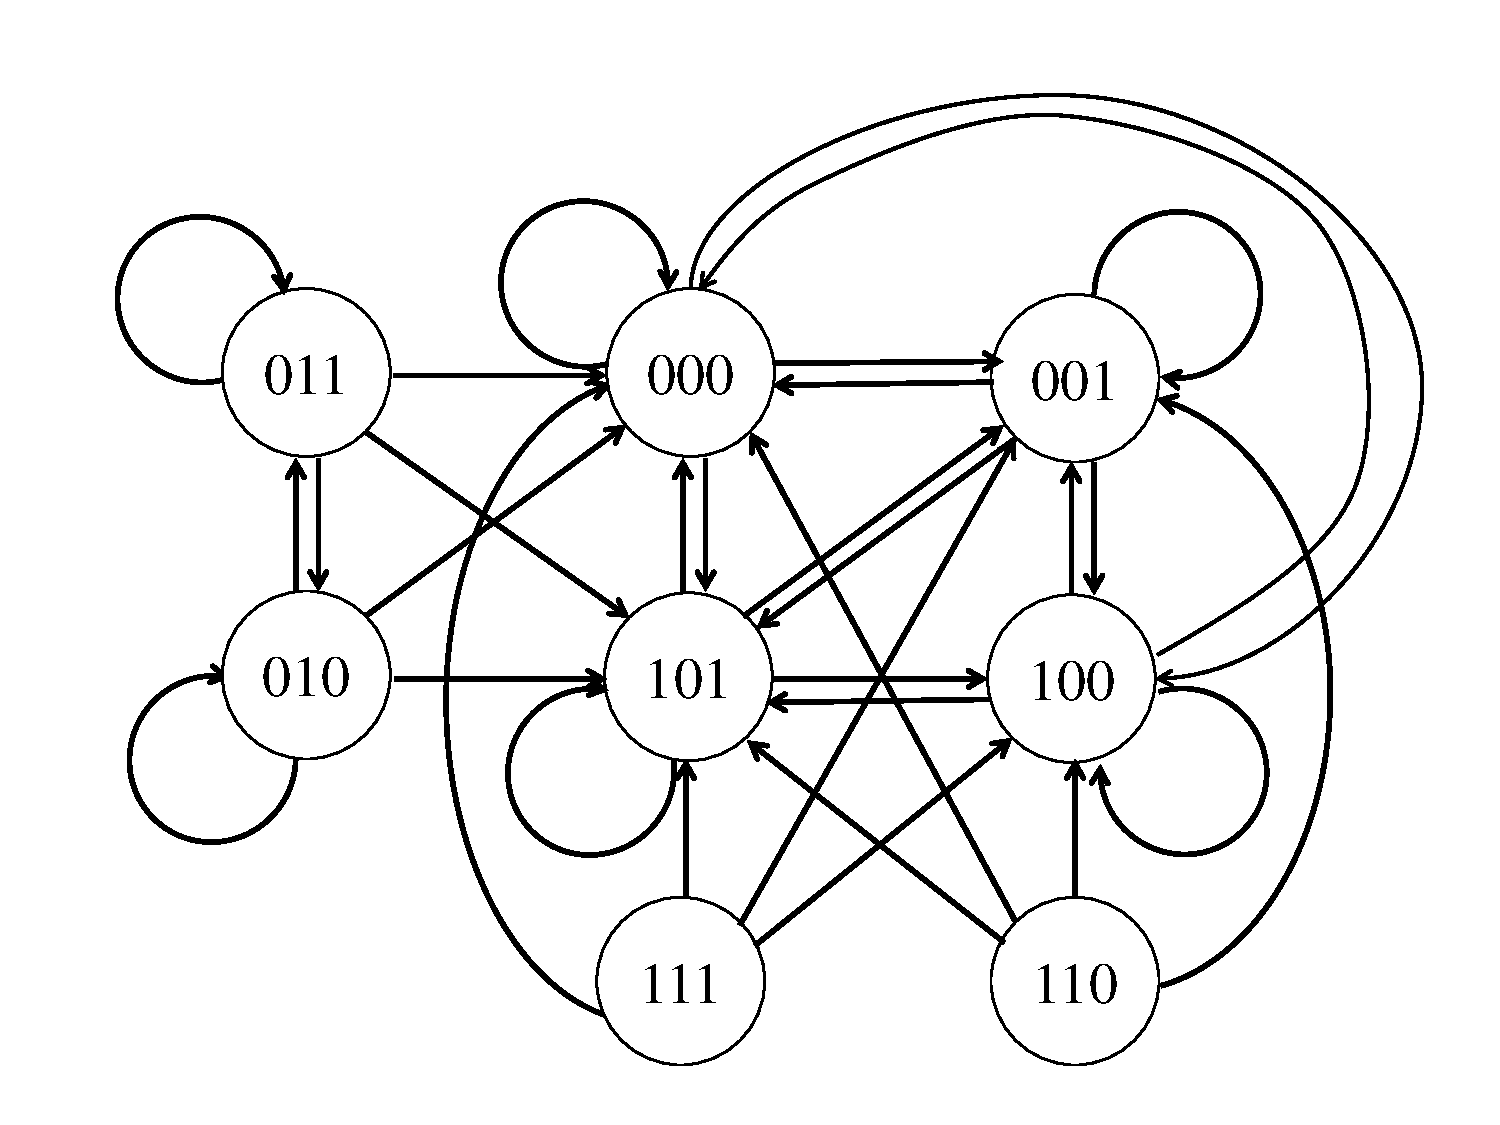
\includegraphics[scale=0.25]{../newfig/s27_stg.pdf}
\end{figure}
\end{column}
\begin{column}{0.5\textwidth}
\begin{figure}
\centering
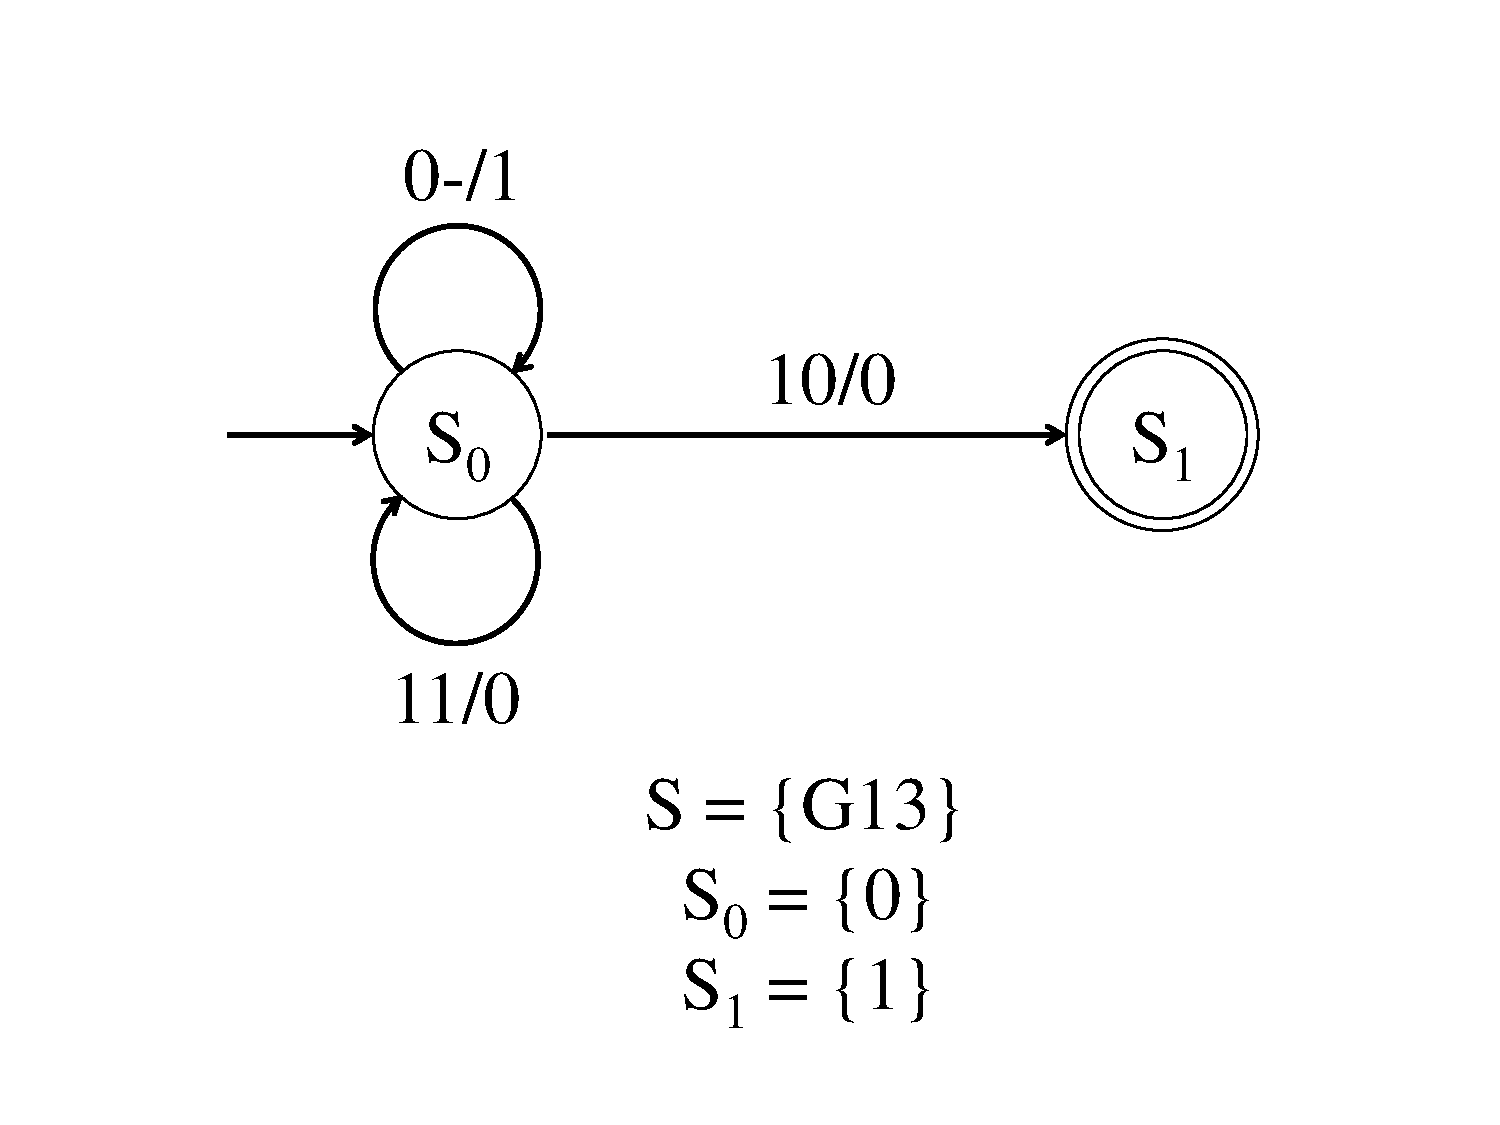
\includegraphics[scale=0.25]{../newfig/s27_stg_refined.pdf}
\end{figure}
\end{column}
\end{columns}
\bi
\item $\{G5/G10 ,G6/G11\}$: irrelevant
\item By removing irrelevant latches, state-space reduced
\ei
\end{frame}
%%%%%%%%%%%%%%%%%%%%%%%%%%%%%%%%%%%%%%%%%%%%%%%%%%%%%%%%%%%%%%
\begin{frame}{\large{Conclusion}}
\bi
\item Word-level abstraction of state-space
\item Apply to reachability analysis
\item Prove effectiveness by experiments on ISCAS'89 and ITC'99 benchmarks
\ei
\pause
\bi
\item Word-level abstraction of function in a single time-frame
\item Word-level unrolling
\item Apply to functional correctness checking of sequential GF multipliers
\item Succeed to verify 162-bit, while contemporary fails beyond 23 bit 
\ei
\pause
\bi
\item UNSAT core extraction for a set of polynomials
\item Refine the core using refutation proof \& syzygies
\item UNSAT core info can be applied to abstraction refinement
\ei
\end{frame}
%%%%%%%%%%%%%%%%%%%%%%%%%%%%%%%%%%%%%%%%%%%%%%%%%%%%%%%%%%%%%%
\begin{frame}{\large{Future work}}
\bi
\item Multivariate polynomial ideals
	\bi
	\item Extend the application of univariate polynomial ideals
	\ei
\ei
\bi
\item Accelerate GB reduction
	\bi
	\item $F_4$ algorithm on term-sparse polynomial ideal (parallel computing)
	\item ZDDs can represent chain of OR gates logic in linear space complexity (alternative canonical graphic representation)
	\ei
\ei
\bi
\item Compute Craig's interpolants using algebraic geometry
	\bi
	\item Projection of varieties $\implies$ interpolants
	\ei
\ei
\end{frame}
%%%%%%%%%%%%%%%%%%%%%%%%%%%%%%%%%%%%%%%%%%%%%%%%%%%%%%%%%%%%%
\begin{frame}{\large{Future work: Craig's interpolants}}
\begin{figure}
\centering
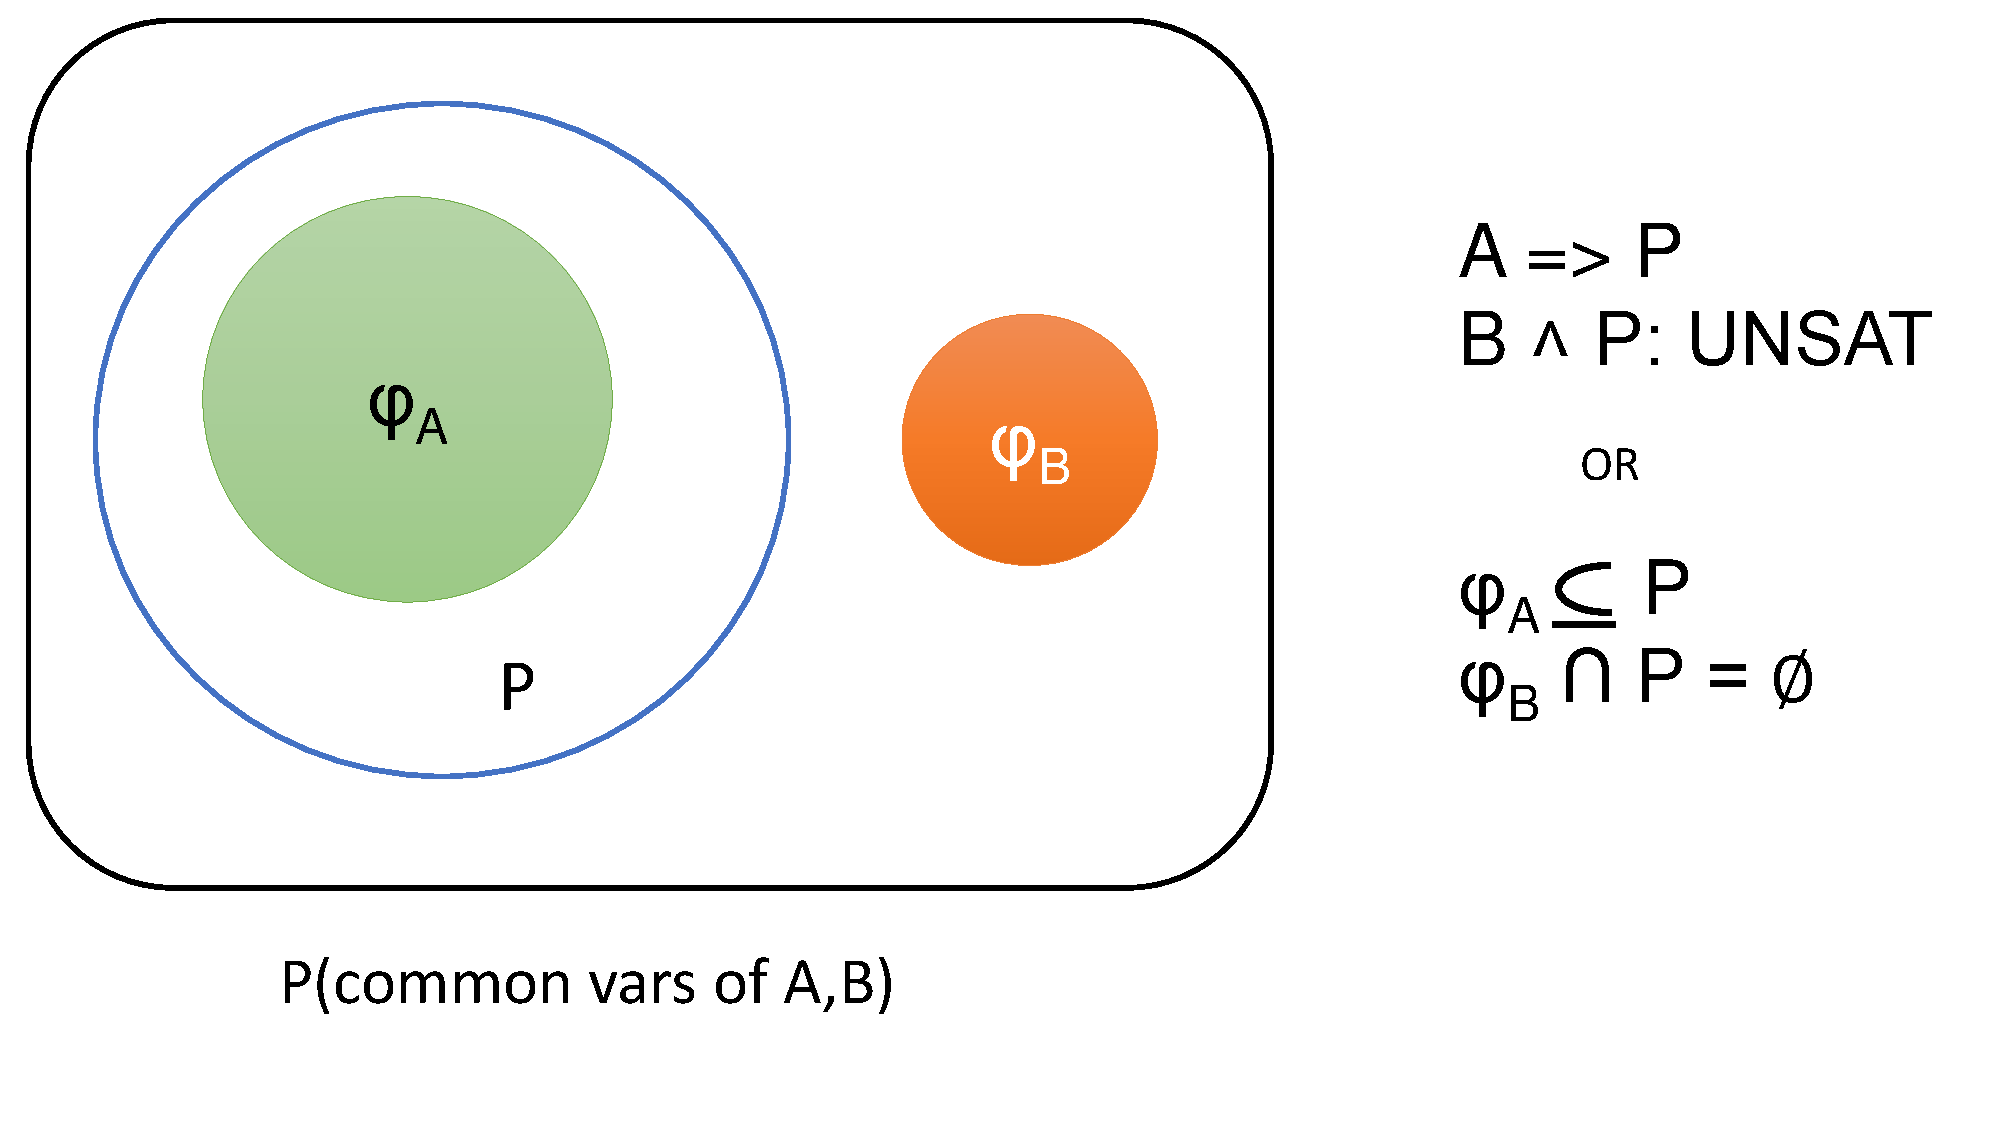
\includegraphics[scale=0.3]{venn_craig.pdf}
\end{figure}
\vspace{-0.2in}
\bi
\item $ A \wedge B = \emptyset$, $A = (\overline{d})(\overline{c})(\overline{a}\vee
d)$ and  $B = (a \vee b \vee c)(\overline{b})$
\item $P = \overline{a}\wedge \overline{c}$ is an interpolant of $(A, B)$
\item Find interpolant from resolution tree [K. Mcmillan '03]
\item Algebraic geometry: projection in affine space
\ei
\end{frame}
%%%%%%%%%%%%%%%%%%%%%%%%%%%%%%%%%%%%%%%%%%%%%%%%%%%%%%%%%%%%%%
\begin{frame}{\large{Publications \& tools}}
\bi
\item Publications:
	\bi
	\item {\it Formal Verification of Sequential Galois Field Arithmetic Circuits using Algebraic Geometry}. {\bf Xiaojun Sun}, Priyank Kalla, Tim Pruss, Florian Enescu. DATE 2015, Grenoble
	\item {\it Finding Unsatisfiable Cores of a Set of Polynomials using the Groebner Basis Algorithm}. {\bf Xiaojun Sun}, Irina Ilioaea, Priyank Kalla, Florian Enescu. CP 2016, Toulouse
	\item {\it Word-level Traversal of Finite States Machines using Algebraic Geometry}. {\bf Xiaojun Sun}, Priyank Kalla, Florian Enescu. HLDVT 2016, Santa Cruz
	\item Journal paper in preparation
	\ei
\item Tools:\\
My website: {\it ece.utah.edu/$\sim$xiaojuns/code.html}
\ei
\end{frame}
%%%%%%%%%%%%%%%%%%%%%%%%%%%%%%%%%%%%%%%%%%%%%%%%%%%%%%%%%%%%%
\begin{frame}{\large{Auf Wiedersehen}}
\begin{figure}
\centering

\includegraphics[scale=0.5]{thankyou.pdf}
\end{figure}
\end{frame}








\end{document}